%% CeTTa: a direct C runtime for the MeTTa family
%%
%% Build:
%%   latexmk -pdf CeTTa.tex     (or pdflatex CeTTa.tex, twice)

\documentclass[11pt]{article}
\usepackage[T1]{fontenc}
\usepackage[utf8]{inputenc}
\usepackage{lmodern}
\usepackage{geometry}
\geometry{margin=1in}
\usepackage{xcolor}
\usepackage[htt]{hyphenat}
\usepackage{hyperref}
\usepackage{longtable}
\usepackage{booktabs}
\usepackage{listings}
\usepackage{multirow}
\usepackage{array}
\usepackage{amsmath}
\newcommand{\eval}[2]{\mathrm{eval}(#1,\,#2)}
\usepackage{amssymb}
\usepackage{tikz}
\usetikzlibrary{arrows.meta,positioning,fit,backgrounds}
\setlength{\emergencystretch}{3em}
\lstset{
  basicstyle=\ttfamily\small,
  breaklines=true,
  frame=single,
  columns=fullflexible,
  keepspaces=true
}
\lstdefinestyle{metta}{
  basicstyle=\ttfamily\small,
  frame=single,
  framerule=0.4pt,
  rulecolor=\color{black!45},
  columns=fullflexible,
  keepspaces=true,
  breaklines=true,
  captionpos=t,
  abovecaptionskip=2pt,
  belowskip=4pt
}
\lstdefinestyle{out}{
  basicstyle=\ttfamily\footnotesize,
  frame=leftline,
  framerule=1.2pt,
  rulecolor=\color{black!30},
  backgroundcolor=\color{black!3},
  columns=fullflexible,
  keepspaces=true,
  breaklines=true,
  aboveskip=2pt,
  belowskip=6pt,
  xleftmargin=4pt
}
\renewcommand{\lstlistingname}{Listing}

\newcommand{\code}[1]{\texttt{#1}}
\newcommand{\outhead}[1]{{\footnotesize\sffamily #1}\par\vspace{1pt}}
\newcommand{\kind}[1]{\textsf{\small[#1]}}
\newcommand{\PeTTa}{\textup{PeTTa}}
\newcommand{\HE}{\textup{HE}}
\newcommand{\CeTTa}{\textup{CeTTa}}
\newcommand{\LeaTTa}{\textup{LeaTTa}}
\newcommand{\PathMap}{\textup{PathMap}}
\newcommand{\RhoCalc}{\textup{RhoCalc}}

\title{\CeTTa{}:\\
\large A Direct C Runtime for the MeTTa Family\\[2pt]
\normalsize How to program it, how it is built, and what each line of
development has achieved}
\author{Zar Goertzel\\Oru\v{z}i}
\date{27 October 2026}

\begin{document}
\maketitle

\begin{abstract}
\CeTTa{} is a direct C runtime for MeTTa, the reflective, nondeterministic
language of the Hyperon framework.  One binary hosts several dialects: \PeTTa{}
(the default, version 1.0.6, with a typed 1.1), \CeTTa{}'s fork of Hyperon
Experimental 0.2.10 with its profile family, and MeTTa Prime, a distinct
language with call by need, call-time choice and a native dependent kernel,
beside the reflective rho calculus, MM2, MeTTa Zero and a HOL Light
proof-stream checker.  This paper is written for a reader who wants to program
\CeTTa{} today.  It teaches the language with listings that run on named
binaries on three lanes, quotes their output, and records where the lanes
differ.  It describes the architecture and the specification-driven
semantics: profiles, oracle conformance, a reflective modal layer, and a
small-step rule table whose rule-removal tests show that the evaluator depends
on the declared rules.  It then gives each line of development its purpose,
history and measured results: the published \code{main}; the opt line, whose
October work realized \code{transform} natively, made space drains linear and
cut the evaluator's cost of crossing between machines; pre-main, which unifies
execution across those machines for the next \code{main}; the native
inference kernel lines; and the Prime families, the draft, the weights, cost
and parallel line, and \code{cetta-ours}, which keeps the live agents running.
For spaces and channels it adopts the direction of an interaction basis: one
atomic commit that observes, keeps or takes, and makes; spaces and channels as
one object that differs only in the rights a holder has; region profiles as
metadata.  The Prime draft runs this basis as a native kernel.  The
reflective rho calculus with its Lean-characterized evaluation at
communication, the cross-runtime benchmark ladder and the abstract-machine
design record are kept, with their dates.
\end{abstract}

%% ────────────────────────────────────────────────────────────────────
\section{Introduction}
\label{sec:intro}

MeTTa~\cite{metta} is a reflective, typed, nondeterministic language
designed as the core language of the OpenCog Hyperon framework.  A MeTTa
program is a space of atoms; equations among those atoms say how expressions
rewrite; a query may have many answers, and the answers form a bag.  Three
families of implementation exist:

\begin{description}
\item[\HE{}] Hyperon Experimental, in Rust, the reference implementation with
  Python bindings and a large standard library (version 0.2.10 is the
  oracle used here).
\item[\PeTTa{}] MeTTa compiled to Prolog clauses and run on SWI-Prolog, a
  dialect of its own with Prolog's search and indexing.
\item[\CeTTa{}] This work: a direct C runtime, now at version 1.5.0-dev on its
  development lines, that runs the \HE{} dialect, the \PeTTa{} dialect (its
  default) and MeTTa Prime from one binary.
\end{description}

\noindent
The dialects share a surface syntax and differ in meaning.  \HE{} leaves an
expression it cannot rewrite as data; \PeTTa{} makes a call that no clause
accepts fail; Prime evaluates by need, so an argument the body never demands
never runs.  A program written for one is not, in general, a program for
another, and \CeTTa{} treats each as a named semantic product with its own
oracle: upstream \HE{} for the \HE{} lane, SWI-\PeTTa{} for the \PeTTa{} lane,
and the Prime metatheory for Prime.

\paragraph{What this paper is for.}  Earlier versions of this paper described
\CeTTa{} through its evidence.  This version is first a guide.
Section~\ref{sec:tutorial} teaches programming in \CeTTa{} with listings run
on all three lanes; Section~\ref{sec:architecture} describes how the runtime
is built; Section~\ref{sec:specdriven} how its semantics is kept honest;
Section~\ref{sec:lines} what each line of development is for and what it has
measured; Sections~\ref{sec:prime-families}, \ref{sec:interaction}
and~\ref{sec:prime} the Prime lines, the interaction basis for spaces and
channels, and the Prime language.  The remaining sections keep the paper's
earlier results, each with its date: the verified \HE{}--\PeTTa{} translation,
the reflective rho calculus, the benchmark ladder and its studies, the
performance analysis, the dialect landscape, the observer-factored account of
nondeterminism and state, the dependent-telescope extension, and the generated
readers.  The appendices record how every listing was run, and keep the
\LeaTTa{} cross-check, the abstract-machine design record and the distilled
principles.

\paragraph{Contributions.}
\begin{enumerate}
\item A tutorial of \CeTTa{}'s MeTTa in which every listing was run on a named
  binary, on the \HE{}, \PeTTa{} and Prime lanes, with the outputs quoted and
  the lanes' differences stated and explained: inert data against failure,
  argument types that decide evaluation, call by need, module destinations,
  the editable standard library with its \code{std:} originals, \code{transform},
  and channels.
\item A specification-driven semantics: explicit profiles; result-bag
  conformance against upstream \HE{} and SWI-\PeTTa{}; a reflective modal
  layer over the one-step relation; a small-step rule table of ten live rule
  classes whose removal tests prove the evaluator depends on them, five of them
  certified in Lean.
\item A history of every line of development with its purpose and measured
  results, among them: on a 96-cell panel against SWI-\PeTTa{} 1.0.6
  (23 October 2026), \CeTTa{}'s \PeTTa{} lane was clearly faster on 78 of 92
  comparable cells and clearly slower on 8; on each of the five programs
  measured on 26 October, the native \code{transform} and its MeTTa library
  ran faster than SWI-\PeTTa{} running the same library; space drains went
  from quadratic to linear.
\item The interaction basis as the direction for spaces and channels, with
  what is proved in Lean, what the Prime draft runs, and what the native
  runtime still lacks.
\item The earlier results, kept and dated: the
  \HE{}$\leftrightarrow$\PeTTa{} translation development (thirteen Lean
  modules with no \code{sorry} in their sources); the reflective rho
  calculus with an axiom-clean Lean characterization of evaluation at
  communication and a funded, receipt-producing cost profile; the
  cross-runtime benchmark ladder; the tail-safe evaluation-arena collector;
  the counted-\PathMap{} backend and its faithful-backend obligations;
  generated readers; MeTTa Zero.
\end{enumerate}

\paragraph{Conventions.}  A \emph{lane} is a language as \CeTTa{} runs it,
selected by \code{-{}-lang}.  Every listing names its lanes, and
Appendix~\ref{app:runs} names the binaries by the first twelve hexadecimal
digits of their SHA-256 digests.  Statements about Prime carry their kind:
\kind{draft} for the behaviour of the C draft, \kind{candidate} for a
property of a candidate design, \kind{direction} for a design direction with
its reasons, \kind{decided} for a recorded decision.  Dates are of 2026.
``Instructions'' are user-mode instructions counted by \code{perf}.

%% ────────────────────────────────────────────────────────────────────
\section{Programming in \CeTTa{}}
\label{sec:tutorial}

This section teaches the language by running it.  Every listing below was run
on the binaries named in Appendix~\ref{app:runs}, and every output panel is
copied from that run.  The same source is run on three \emph{lanes}: \CeTTa{}'s
\HE{} lane (\code{-{}-lang he}), its \PeTTa{} lane (\code{-{}-lang petta}, the
default) and the Prime lane (\code{-{}-lang prime}).  The lanes are distinct
dialects that share a surface syntax.  Where a listing behaves differently on
two lanes, the text says so and says why; nothing in this section assumes that
a program written for one lane runs the same on another.

\subsection{Running a program}
\label{sec:tut-running}

One executable, \code{cetta}, hosts every language.  The \code{-{}-lang} option
selects it:

\begin{lstlisting}[style=metta]
cetta program.metta                    # PeTTa 1.0.6, the default
cetta --lang petta@1.1 program.metta   # PeTTa with static typing
cetta --lang he program.metta          # CeTTa's fork of Hyperon Experimental 0.2.10
cetta --lang he --profile extended program.metta
cetta --lang prime program.metta       # MeTTa Prime
cetta --lang rhocalc program.rho       # the reflective rho calculus
\end{lstlisting}

\noindent
The binary also carries an MM2 front end, the MeTTa Zero kernel and its
relatives, and a native HOL Light proof-stream checker; \code{cetta
-{}-list-languages} prints the inventory and \code{cetta -{}-help} the options.
The binary built from \code{main} (1.4.0-dev) defaults to the \HE{} lane;
\PeTTa{} became the default on 17 October, in the 1.5 line.

A program is a sequence of atoms.  An atom is a symbol (\code{red}), a
variable (\code{\$x}), a grounded value (a number or a string) or an
expression, a parenthesized sequence of atoms.  A top-level atom is added to
the program's own space, \code{\&self}; a top-level \code{!(\ldots)} is a
query, evaluated in place, whose answers are printed.  The lanes print
differently.  \HE{} and Prime print the answers of one query as one bracketed
list, \code{[a, b]}, and an effect that returns the unit value prints as
\code{[()]}.  \PeTTa{} prints one line per answer and \code{true} for an
effect.  Comments run from \code{;} to the end of the line.  The option
\code{-{}-pretty-vars} prints fresh variables by their written names; the
listings use it.

\subsection{Equations and evaluation}
\label{sec:tut-equations}

An equation \code{(= lhs rhs)} says that an atom matching \code{lhs} may be
rewritten to \code{rhs}.  Evaluating a call looks up the equations whose
left side matches it, instantiates their right sides and evaluates those in
turn.  Grounded operations such as \code{+} and \code{*} compute directly.

\begin{lstlisting}[style=metta,caption={Equations and evaluation; all three lanes},label={lst:t01}]
; Equations are atoms of the program space; a call rewrites by them.
(= (double $x) (* 2 $x))
(= (len ()) 0)
(= (len (Cons $h $t)) (+ 1 (len $t)))
(= (fact $n) (if (== $n 0) 1 (* $n (fact (- $n 1)))))
!(double 21)
!(len (Cons a (Cons b (Cons c ()))))
!(fact 20)
; a call no equation matches
!(len nothing)
\end{lstlisting}
\noindent\begin{minipage}[t]{0.32\textwidth}
\outhead{HE lane}
\begin{lstlisting}[style=out]
[42]
[3]
[2432902008176640000]
[(len nothing)]
\end{lstlisting}
\end{minipage}\hfill
\begin{minipage}[t]{0.32\textwidth}
\outhead{PeTTa lane}
\begin{lstlisting}[style=out]
42
3
2432902008176640000
\end{lstlisting}
\end{minipage}\hfill
\begin{minipage}[t]{0.32\textwidth}
\outhead{Prime lane}
\begin{lstlisting}[style=out]
[42]
[3]
[2432902008176640000]
[(len nothing)]
\end{lstlisting}
\end{minipage}

\noindent
The three lanes agree on every computed answer.  They disagree on the last
query, and the disagreement is a real difference between the dialects.  On the
\HE{} and Prime lanes an expression that no equation rewrites is its own
normal form: \code{(len nothing)} stays as data.  This is MeTTa's rule that
what cannot be interpreted is left uninterpreted.  On the \PeTTa{} lane a
function is compiled to Prolog clauses, and a call that no clause of a
\emph{defined} function accepts fails: it has no answer.  SWI-\PeTTa{}, the
reference implementation of the dialect, gives the same output on this
listing and on the six \PeTTa{}-lane listings of
Sections~\ref{sec:tut-nondet}--\ref{sec:tut-modules}, up to the spelling of
fresh variables (\code{\$V0} against \code{\$\_0}).

\subsection{Several answers, and the bag they form}
\label{sec:tut-nondet}

A call may match several equations.  Each match is a separate answer, and a
query prints them all.  \code{superpose} makes the answers of a list, and
\code{collapse} does the reverse: it evaluates its argument completely and
returns one expression holding every answer.

\begin{lstlisting}[style=metta,caption={Several answers, and the bag they form},label={lst:t02}]
; Several equations for one call give several answers.
(= (color) red)
(= (color) green)
(= (color) blue)
!(color)
; collapse turns the answers into one expression: the bag, as a value
!(collapse (color))
!(let $x (superpose (1 2 3)) (* $x $x))
; duplicates are real occurrences
!(collapse (superpose (a b a)))
; an order-insensitive view of a bag
!(let $bag (collapse (superpose (c a b))) (sort-atom $bag))
; a head with no equations at all is data
!(undefined-head 1)
\end{lstlisting}
\noindent\begin{minipage}[t]{0.32\textwidth}
\outhead{HE lane}
\begin{lstlisting}[style=out]
[red, green, blue]
[(red green blue)]
[1, 4, 9]
[(a b a)]
[(a b c)]
[(undefined-head 1)]
\end{lstlisting}
\end{minipage}\hfill
\begin{minipage}[t]{0.32\textwidth}
\outhead{PeTTa lane}
\begin{lstlisting}[style=out]
red
green
blue
(red green blue)
1
4
9
(a b a)
(a b c)
(undefined-head 1)
\end{lstlisting}
\end{minipage}\hfill
\begin{minipage}[t]{0.32\textwidth}
\outhead{Prime lane}
\begin{lstlisting}[style=out]
[red, green, blue]
[(red green blue)]
[1, 4, 9]
[(a b a)]
[(a b c)]
[(undefined-head 1)]
\end{lstlisting}
\end{minipage}

\noindent
The collection of answers is a \emph{bag}: a multiset, in which duplicates are
real occurrences (\code{(a b a)} keeps both copies of \code{a}) and the order
in which an engine happens to find the answers carries no meaning.  A printed
result is necessarily a sequence, but programs and tests should not depend on
it; the conformance gates of Section~\ref{sec:conformance} compare bags.  When
a program wants a canonical sequence, it sorts the bag explicitly, as the
fifth query does.  A program written for one engine may still exploit that
engine's documented order; it then says so by being engine-specific.

The fifth query binds the bag with \code{let} before sorting it, and this
matters on the \HE{} lane.  There, a declared argument type of
\code{Expression} or \code{Atom} tells the evaluator \emph{not} to evaluate
that argument, and \code{sort-atom} is declared
\code{(-> Expression Expression)}:

\begin{lstlisting}[style=metta,caption={Argument types decide evaluation on the HE lane},label={lst:t02b}]
; sort-atom is declared (-> Expression Expression) on the HE lane
!(get-type sort-atom)
!(sort-atom (c a b))
; written directly, the argument is not evaluated first
!(sort-atom (collapse (superpose (c a b))))
; bound with let first, the bag is sorted
!(let $bag (collapse (superpose (c a b))) (sort-atom $bag))
\end{lstlisting}
\noindent\begin{minipage}[t]{0.32\textwidth}
\outhead{HE lane}
\begin{lstlisting}[style=out]
[(-> Expression Expression)]
[(a b c)]
[(c a b)]
[(a b c)]
\end{lstlisting}
\end{minipage}\hfill
\begin{minipage}[t]{0.32\textwidth}
\outhead{PeTTa lane}
\begin{lstlisting}[style=out]
%Undefined%
(a b c)
(a b c)
(a b c)
\end{lstlisting}
\end{minipage}\hfill
\begin{minipage}[t]{0.32\textwidth}
\outhead{Prime lane}
\begin{lstlisting}[style=out]
[(-> Expression Expression)]
[(a b c)]
[(a b c)]
[(a b c)]
\end{lstlisting}
\end{minipage}

\noindent
Written directly, \code{(sort-atom (collapse \ldots))} sorts the
\emph{unevaluated} expression \code{(collapse (superpose (c a b)))} and only
then evaluates the result, so the bag comes out unsorted.  On the \PeTTa{}
and Prime lanes \code{sort-atom} evaluates its argument first, although Prime
declares the same type.  On the \HE{}
lane the type of a function decides which of its arguments are evaluated, and
\code{let} is the portable way to force a value before a call.  A
user-defined function with a parameter typed \code{Atom} receives that
argument unevaluated on the \HE{} and \PeTTa{} lanes alike (SWI-\PeTTa{}
agrees), but not on the Prime lane (Section~\ref{sec:prime}).

\subsection{Demand and call-time choice}
\label{sec:tut-demand}

The \HE{} and \PeTTa{} lanes are eager: arguments are evaluated before a
function's equations are tried.  Prime evaluates by need: an argument is
evaluated only when the chosen equation demands it, and then at most once.

\begin{lstlisting}[style=metta,caption={Demand and call-time choice},label={lst:t03}]
(= (const $x $y) $x)
(= (pair $x) ($x $x))
; is an argument the body never needs evaluated?
!(const 5 (println! "argument evaluated"))
; one choice, used twice
!(pair (superpose (1 2)))
\end{lstlisting}
\noindent\begin{minipage}[t]{0.32\textwidth}
\outhead{HE lane}
\begin{lstlisting}[style=out]
argument evaluated
[5]
[(1 1), (2 2)]
\end{lstlisting}
\end{minipage}\hfill
\begin{minipage}[t]{0.32\textwidth}
\outhead{PeTTa lane}
\begin{lstlisting}[style=out]
"argument evaluated"
5
(1 1)
(2 2)
\end{lstlisting}
\end{minipage}\hfill
\begin{minipage}[t]{0.32\textwidth}
\outhead{Prime lane}
\begin{lstlisting}[style=out]
[5]
[(1 1), (2 2)]
\end{lstlisting}
\end{minipage}

\noindent
\code{const} never uses its second argument, so on the Prime lane the
\code{println!} never runs; on the eager lanes it runs before \code{const} is
entered.  The second query shows \emph{call-time choice}: the argument
\code{(superpose (1 2))} is one choice, shared by both uses of \code{\$x}, so
the answers are \code{(1 1)} and \code{(2 2)}, never \code{(1 2)}.  The eager
lanes give the same answers for a different reason: they choose before the
call.  Under call by need the sharing is the semantics: a delayed argument is
one \emph{need cell}, and every use of it sees the same value
(Section~\ref{sec:prime}).

\subsection{Spaces: \code{match}, \code{add-atom}, \code{remove-atom}}
\label{sec:tut-spaces}

A \emph{space} is a store of atoms.  \code{new-space} makes one and
\code{bind!} gives it a name; \code{add-atom} and \code{remove-atom} change it;
\code{(match space pattern template)} answers one instance of the template
for each stored atom that matches the pattern.  A comma pattern
\code{(, p1 p2)} is a conjunction: both patterns must match, with shared
variables bound alike.  The program space is a space like any other, and its
equations are atoms in it.

\begin{lstlisting}[style=metta,caption={Spaces, queries and updates},label={lst:t04}]
!(bind! &kb (new-space))
!(add-atom &kb (parent tom bob))
!(add-atom &kb (parent bob ann))
!(add-atom &kb (parent bob jim))
; match: one answer per matching occurrence
!(match &kb (parent bob $c) $c)
; a conjunctive query
!(match &kb (, (parent $g $p) (parent $p $c)) (grandparent $g $c))
(= (children $p) (collapse (match &kb (parent $p $c) $c)))
!(children bob)
!(remove-atom &kb (parent bob jim))
!(children bob)
; the program space is a space too: equations are atoms in it
(= (double $x) (* 2 $x))
!(match &self (= (double $x) $body) $body)
\end{lstlisting}
\noindent\begin{minipage}[t]{0.32\textwidth}
\outhead{HE lane}
\begin{lstlisting}[style=out]
[()]
[()]
[()]
[()]
[ann, jim]
[(grandparent tom ann), (grandparent tom jim)]
[(ann jim)]
[()]
[(ann)]
[(* 2 $x)]
\end{lstlisting}
\end{minipage}\hfill
\begin{minipage}[t]{0.32\textwidth}
\outhead{PeTTa lane}
\begin{lstlisting}[style=out]
true
true
true
ann
jim
(grandparent tom ann)
(grandparent tom jim)
(ann jim)
true
(ann)
(* 2 $V0)
\end{lstlisting}
\end{minipage}\hfill
\begin{minipage}[t]{0.32\textwidth}
\outhead{Prime lane}
\begin{lstlisting}[style=out]
[()]
[()]
[()]
[()]
[ann, jim]
[(grandparent tom ann), (grandparent tom jim)]
[(bob ann jim)]
[()]
[(bob ann)]
[(* 2 $x)]
\end{lstlisting}
\end{minipage}

\noindent
The lanes agree, with one exception that is a defect of the current Prime
draft, not a property of Prime.  On the Prime lane, \code{(children bob)}
answers \code{(bob ann jim)}: inside \code{match}, the pattern variable
\code{\$p} is treated as a fresh variable even though the call has bound it to
\code{bob}, so the query matches every parent.  The same probe gives the same
answer on both draft binaries of Appendix~\ref{app:runs}.  The deviation was
found by the interaction study of Section~\ref{sec:interaction} and is listed
among the draft's open repairs in Section~\ref{sec:prime-draft} \kind{draft};
the interaction form \code{transform} respects outer bindings.

\subsection{Types}
\label{sec:tut-types}

A type declaration \code{(: atom type)} is itself an atom of the space.
Arrow types \code{(-> A B C)} type functions.  What a lane does with a
declaration differs more than anything else in this section.

\begin{lstlisting}[style=metta,caption={Declared types and an ill-typed call},label={lst:t05}]
(: Nat Type)
(: Z Nat)
(: S (-> Nat Nat))
(: add (-> Nat Nat Nat))
(= (add Z $y) $y)
(= (add (S $x) $y) (S (add $x $y)))
!(add (S Z) (S (S Z)))
!(get-type (S Z))
!(get-type add)
; an argument of the wrong type
!(add (S Z) "two")
\end{lstlisting}
\noindent\begin{minipage}[t]{0.32\textwidth}
\outhead{HE lane}
\begin{lstlisting}[style=out]
[(S (S (S Z)))]
[Nat]
[(-> Nat Nat Nat)]
[(Error (add (S Z) "two") (BadArgType 2 Nat String))]
\end{lstlisting}
\end{minipage}\hfill
\begin{minipage}[t]{0.32\textwidth}
\outhead{PeTTa lane}
\begin{lstlisting}[style=out]
(S (S (S Z)))
Nat
(-> Nat Nat Nat)
\end{lstlisting}
\end{minipage}\hfill
\begin{minipage}[t]{0.32\textwidth}
\outhead{Prime lane}
\begin{lstlisting}[style=out]
[(S (S (S Z)))]
[Nat]
[(-> Nat Nat Nat)]
[(Error (add (S Z) "two") (BadArgType 2 Nat String))]
\end{lstlisting}
\end{minipage}

\noindent
The \HE{} and Prime lanes check the call and answer an error value,
\code{(Error \ldots (BadArgType 2 Nat String))}, which is ordinary data that a
program can match.  The default \PeTTa{} lane checks argument types when the
call runs and makes an ill-typed call fail, so the last query has no answer;
SWI-\PeTTa{} agrees.  The typed \PeTTa{} 1.1 lane checks the whole program
before running any of it and rejects it:

\noindent\begin{minipage}[t]{0.98\textwidth}
\outhead{PeTTa 1.1 lane}
\begin{lstlisting}[style=out]
PeTTa type error: Type mismatch: call arguments conflict with inferred type for add
\end{lstlisting}
\end{minipage}

\noindent
Two further typed products exist on the \PeTTa{} side, the
\code{typecheck-v2} and \code{typecheck-v3} profiles of
Section~\ref{sec:petta-typecheck}.  Prime's typing is its own and never
defers to \HE{}'s type engine \kind{decided}; Section~\ref{sec:prime}
describes its faces.

\subsection{Modules and imports}
\label{sec:tut-modules}

\code{import!} loads a file of atoms.  With \code{\&self} as its destination
the atoms join the program space.  A module name is resolved relative to the
importing file.  Libraries shipped with the binary are named
\code{(library name)} on the \PeTTa{} lane, and by their module name on the
\HE{} and Prime lanes (\code{!(import! \&self lts:he)},
\code{!(import! \&self interaction)}).

\begin{lstlisting}[style=metta,caption={Importing a module file},label={lst:t06}]
; load a module file into the program space
!(import! &self lib/geometry)
!(square 7)
!(area (rect 3 4))
\end{lstlisting}
\noindent\begin{minipage}[t]{0.32\textwidth}
\outhead{HE lane}
\begin{lstlisting}[style=out]
[()]
[49]
[12]
\end{lstlisting}
\end{minipage}\hfill
\begin{minipage}[t]{0.32\textwidth}
\outhead{PeTTa lane}
\begin{lstlisting}[style=out]
true
49
12
\end{lstlisting}
\end{minipage}\hfill
\begin{minipage}[t]{0.32\textwidth}
\outhead{Prime lane}
\begin{lstlisting}[style=out]
[()]
[49]
[12]
\end{lstlisting}
\end{minipage}

\noindent
A module can also be loaded into a space of its own and queried there.  On the
\HE{} and Prime lanes the destination must then be \code{\&self} or a name not
yet bound; \code{import!} creates the space.  Importing into a space bound
earlier with \code{bind!} is refused with an error value.  The \PeTTa{} lane
accepts either form.

\begin{lstlisting}[style=metta,caption={Importing a module into a space of its own},label={lst:t06b}]
; load a module into a fresh space of its own, then query it
!(import! &geo lib/geometry)
!(match &geo (= (square $x) $body) $body)
\end{lstlisting}
\noindent\begin{minipage}[t]{0.32\textwidth}
\outhead{HE lane}
\begin{lstlisting}[style=out]
[()]
[(* $x $x)]
\end{lstlisting}
\end{minipage}\hfill
\begin{minipage}[t]{0.32\textwidth}
\outhead{PeTTa lane}
\begin{lstlisting}[style=out]
true
(* $V0 $V0)
\end{lstlisting}
\end{minipage}\hfill
\begin{minipage}[t]{0.32\textwidth}
\outhead{Prime lane}
\begin{lstlisting}[style=out]
[()]
[(* $x $x)]
\end{lstlisting}
\end{minipage}

\subsection{The standard library, and redefining it}
\label{sec:tut-stdlib}

Every lane ships a standard library: list and expression operations
(\code{car-atom}, \code{cdr-atom}, \code{size-atom}, \code{sort-atom},
\code{foldl-atom}), numeric and string operations, space operations, and
control (\code{if}, \code{case}, \code{let}, \code{let*}, \code{collapse},
\code{superpose}).  It is precompiled into the binary, so a program starts
without parsing it: a one-line query completes in under ten milliseconds at
about 14\,MB of peak memory on the \HE{} and \PeTTa{} lanes (single runs).

What happens when a program defines an equation for a library name differs by
lane.  On the \HE{} lane the grounded operation wins and the program's
equation is never consulted.  On the \PeTTa{} lane, as in SWI-\PeTTa{}, the
library function is a static Prolog procedure, and the program's equation is
refused with a permission error:

\begin{lstlisting}[style=metta,caption={Adding an equation for a builtin on the HE and PeTTa lanes},label={lst:t07b}]
(= (size-atom $x) many)
!(collapse (size-atom (a b c)))
!(std:size-atom (a b c))
\end{lstlisting}
\noindent\begin{minipage}[t]{0.485\textwidth}
\outhead{HE lane}
\begin{lstlisting}[style=out]
[(3)]
[(std:size-atom (a b c))]
\end{lstlisting}
\end{minipage}\hfill
\begin{minipage}[t]{0.485\textwidth}
\outhead{PeTTa lane}
\begin{lstlisting}[style=out]
error: (Error (permission_error modify static_procedure (/ size-atom 2)) (context (: system (/ assertz 2)) $_))
\end{lstlisting}
\end{minipage}

\noindent
The Prime draft makes the standard definitions ordinary, editable occurrences
of the program space and keeps the originals under the \code{std:} prefix
\kind{draft}, since 26 October 2026.  An added equation is one more
alternative; removing the standard rows removes their behaviour;
\code{(std:definitions name)} returns the original declarations and equations
as data, and re-adding them restores the original.  A qualified call such as
\code{std:size-atom} always reaches the original implementation:

\begin{lstlisting}[style=metta,caption={Editing a standard definition on the Prime lane},label={lst:t07}]
; Standard definitions are ordinary, editable occurrences of the program
; space; std: names keep the originals.
!(size-atom (a b c))
!(std:size-atom (a b c))
!(collapse (std:definitions size-atom))
; add an alternative: a second answer for every call
(= (size-atom $x) many)
!(collapse (size-atom (a b c)))
!(std:size-atom (a b c))
; remove the standard rows: only the program's equation is left
!(let $d (std:definitions size-atom) (remove-atom &self $d))
!(collapse (size-atom (a b c)))
; restore them
!(let $d (std:definitions size-atom) (add-atom &self $d))
!(collapse (size-atom (a b c)))
\end{lstlisting}
\noindent\begin{minipage}[t]{0.98\textwidth}
\outhead{Prime lane}
\begin{lstlisting}[style=out]
[3]
[3]
[((: size-atom (-> Expression Number)) (= (size-atom $argument0) (std:size-atom $argument0)))]
[(3 many)]
[3]
[(), ()]
[(many)]
[(), ()]
[(many 3)]
\end{lstlisting}
\end{minipage}

\noindent
After the restoration the bag is \code{(many 3)}: the program's equation now
precedes the restored rows, and occurrence order is observable in the printed
sequence, though not in the bag.  The native implementation of a standard
operation is used only while the definitions it stands for are unchanged; an
edited operation goes through ordinary equation evaluation.

\subsection{\code{transform}: one atomic step over a space}
\label{sec:tut-transform}

\code{match} reads and \code{add-atom}/\code{remove-atom} write, one at a time.
A program that must consume a job exactly once, or move money between two
accounts, needs to read, consume and produce in one indivisible step.
\code{transform} is that step.  Its sources are patterns, each marked by what
the step does with the matched occurrence:

\begin{itemize}
\item a plain pattern or \code{(read p)} \emph{keeps} it (reads it and leaves it);
\item \code{(take p)} \emph{takes} it (consumes it);
\item \code{(absent p)}, \code{(unique p)} and \code{(all p P)} are
  \emph{predicate queries}: they look at the whole space (no match, exactly one,
  every match) and dispose of nothing;
\item \code{(every c)} fires every match of \code{c} in the same step;
\item \code{(let P E)} evaluates \code{E} once the sources have bound its
  variables, and contributes no row when it has no value.
\end{itemize}

\noindent
The template is instantiated once per fired row.  With a destination space as
fourth argument the instances are added there and the answer is how many; with
none they are answered to the caller.  On the \PeTTa{} lane the operation is a
library, \code{lib\_transform}, written in MeTTa, and the binary fires it
natively when the library is the unmodified one:

\begin{lstlisting}[style=metta,caption={\code{transform} on the PeTTa lane},label={lst:t08}]
!(import! &self (library lib_transform))
!(bind! &s (new-space))
!(add-atom &s (job 1))
!(add-atom &s (job 2))
!(add-atom &s (rate 3))
; take one job and keep the rate, in one step
!(transform &s (, (rate $r) (take (job $n))) (priced $n $r))
; every: all remaining matches fire in this one commit
!(transform &s (every (take (job $n))) (done $n))
!(collapse (match &s (job $n) $n))
; absent: a predicate query; here a closure that adds each path once
!(bind! &g (new-space))
!(add-atom &g (edge a b))
!(add-atom &g (edge b c))
!(transform &g (every (, (edge $x $y) (absent (path $x $y)))) (path $x $y) &g)
!(transform &g (every (, (path $x $y) (edge $y $z) (absent (path $x $z)))) (path $x $z) &g)
!(transform &g (every (, (path $x $y) (edge $y $z) (absent (path $x $z)))) (path $x $z) &g)
!(sort-atom (collapse (match &g (path $x $y) ($x $y))))
\end{lstlisting}
\noindent\begin{minipage}[t]{0.32\textwidth}
\outhead{PeTTa lane}
\begin{lstlisting}[style=out]
true
true
true
true
(priced 1 3)
(done 2)
()
true
true
2
1
0
((a b) (a c) (b c))
\end{lstlisting}
\end{minipage}\hfill
\begin{minipage}[t]{0.32\textwidth}
\outhead{PeTTa lane, authored firing}
\begin{lstlisting}[style=out]
true
true
true
true
(priced 1 3)
(done 2)
()
true
true
2
1
0
((a b) (a c) (b c))
\end{lstlisting}
\end{minipage}\hfill
\begin{minipage}[t]{0.32\textwidth}
\outhead{SWI-PeTTa}
\begin{lstlisting}[style=out]
true
true
true
true
(priced 1 3)
(done 2)
()
true
true
2
1
0
((a b) (a c) (b c))
\end{lstlisting}
\end{minipage}

\noindent
The first step keeps the rate and takes job~1; the \code{every} step takes
every remaining job; the closure adds each path once, guarded by
\code{absent}, and the third round adds nothing.  The native firing, the
authored firing in the library (forced with an environment switch), and
SWI-\PeTTa{} running the same library file all leave the same answers and the
same space.  Section~\ref{sec:line-opt} describes how the native realization
was built and measured.

\subsection{Processes and channels}
\label{sec:tut-processes}

\paragraph{One interaction form on the Prime lane.}
On the Prime lane the draft implements the interaction form of
Section~\ref{sec:interaction} as a native kernel with a MeTTa library,
imported as the module \code{interaction} \kind{draft}.  A step reads, keeps,
takes and makes in one atomic \emph{commit}, across any number of spaces.
\emph{Regions} made by \code{new-region} carry a profile (space, channel,
mailbox, log or board) that fixes which of the four parts each holder may
perform; a commit outside its holder's rights is not formed.  \code{await}
parks a step until it can fire and fires it once; \code{whenever} installs it
as a rule that fires on every enabling; Rholang's receipts
(\code{for} with \code{<-}, \code{<=}, \code{<<-}) are aliases of these.

\begin{lstlisting}[style=metta,caption={One interaction form on the Prime lane: commits, regions, waiting},label={lst:t09}]
!(import! &self interaction)
!(bind! &s (new-space))
!(add-atom &s (job 1))
!(add-atom &s (rate 3))
; one commit: keep the rate, take the job, make the result
!(transform &s (, (read (rate $r)) (take (job $n))) (priced $n $r))
; a row never reads and takes the same occurrence
!(add-atom &s Token)
!(transform &s (, (read Token) (take Token)) committed)
!(add-atom &s Token)
!(transform &s (, (read Token) (take Token)) committed)
; regions: a channel has no predicate queries, for anyone
!(let $c (new-region channel) (rights-of $c))
!(let $c (new-region channel) (transform $c (absent (msg $x)) empty))
; waiting: await parks until the commit can fire, then fires once
!(bind! &q (new-space))
!(bind! &out (new-space))
!(await (transform &q (take (job $x)) (add-atom &out (got $x))))
!(transform &q () (, (add-atom &q (job 1)) (add-atom &q (job 2))))
!(collapse (match &out (got $x) $x))
; whenever: a rule that fires on every enabling
!(whenever (transform &q (take (job $x)) (add-atom &out (served $x))))
!(transform &q () (add-atom &q (job 3)))
!(sort-atom (collapse (match &out (served $x) $x)))
; Rholang's receipt, as an alias of await over a take
!(bind! &c2 (new-space))
!(for ((msg $m) <- &c2) (add-atom &out (heard $m)))
!(transform &c2 () (add-atom &c2 (msg hello)))
!(collapse (match &out (heard $m) $m))
\end{lstlisting}
\noindent\begin{minipage}[t]{0.98\textwidth}
\outhead{Prime lane}
\begin{lstlisting}[style=out]
[()]
[()]
[()]
[()]
[(priced 1 3)]
[()]
[()]
[committed]
[(receive peek send)]
[(Error transform (not-formed (missing-right observe (Sealed region))))]
[()]
[()]
[()]
[()]
[(1)]
[()]
[()]
[(2 3)]
[()]
[()]
[()]
[(hello)]
\end{lstlisting}
\end{minipage}

\noindent
The first commit keeps the rate and takes the job.  The two
\code{(read Token) (take Token)} steps show \emph{identification}: one row may
not keep and take the same occurrence, so with one token nothing commits (the
step answers \code{()}), and with two it does.  A channel region has no predicate
queries, so \code{absent} on it is not formed, whatever the holder.  The
\code{await} fires once, on job~1; the rule installed by \code{whenever}
serves the remaining job~2 and then job~3 as it arrives; and the receipt
written with \code{for} is woken by the send.  These are the semantics of the
interaction study, run on the draft binary; the trusted part is a small
kernel, and the meaning is stated beside it in the library.

\paragraph{The reflective rho calculus.}
\code{-{}-lang rhocalc} runs the reflective higher-order rho calculus of
Section~\ref{sec:rhocalc}.  A process sends on a name with \code{x!(P)} and
receives with \code{for (\$y <- x) \{Q\}}; \code{@\{P\}} quotes a process into
a name and \code{*\$y} runs the process a name quotes.  The one reduction,
COMM, consumes a send and a receive on the same name.  When the message is
itself code and the receiver runs it, a communication is an evaluation step:

\begin{lstlisting}[style=metta,caption={Evaluation at COMM in the strict-core rho calculus},label={lst:t10}]
// Eval at COMM: running code you were sent, with no execution primitive.
//
// The rho-calculus has no "run" instruction.  A quoted process is inert
// data -- until it is communicated.  The runner idiom makes execution cost
// exactly one handshake:
//
//     run!(P) | for ($y <- run) { *$y }   --COMM-->   P
//
// The send carries the program P as data (the engine quotes it on the
// wire); the receiver drops (runs) whatever arrives.  Channels are quoted
// processes, so run = @{0} and out = @{@{0}!(0)} are two distinct names.
//
// Here P = out!(0) is itself a send that completes a second handshake with
// a receiver already waiting on out.  The whole program settles at 0 only
// if the delivered code actually ran: first COMM delivers P, the drop
// activates it, and the second COMM consumes it.
//
// Run: ./cetta --lang rhocalc examples/rho/pure/eval_at_comm.rho
// Expected: 0

@{0}!(@{@{0}!(0)}!(0)) |
for ($y <- @{0}) {*$y} |
for ($r <- @{@{0}!(0)}) {0}
\end{lstlisting}
\noindent\begin{minipage}[t]{0.98\textwidth}
\outhead{\code{-{}-lang rhocalc}}
\begin{lstlisting}[style=out]
0
\end{lstlisting}
\end{minipage}

\noindent
The program settles at \code{0} only if the delivered code ran: the first COMM
delivers the send \code{@\{@\{0\}!(0)\}!(0)}, the drop activates it, and the
second COMM consumes it.  Without the last receiver the activated send is
left over:

\begin{lstlisting}[style=metta,caption={The same program without the last receiver},label={lst:t10c}]
@{0}!(@{@{0}!(0)}!(0)) |
for ($y <- @{0}) {*$y}
\end{lstlisting}
\noindent\begin{minipage}[t]{0.98\textwidth}
\outhead{\code{-{}-lang rhocalc}}
\begin{lstlisting}[style=out]
@{@{0}!(0)}!(0)
\end{lstlisting}
\end{minipage}

\subsection{What the listings show about the lanes}
\label{sec:tut-summary}

\begin{center}
\small
\begin{tabular}{@{}p{0.27\linewidth}p{0.20\linewidth}p{0.20\linewidth}p{0.25\linewidth}@{}}
\toprule
Behaviour & \HE{} lane & \PeTTa{} lane & Prime lane \\
\midrule
call no equation of a defined head matches & inert data & no answer & inert data \\
parameter typed \code{Atom} & held & held & evaluated; \code{(Data Atom)} holds \kind{draft} \\
unneeded argument & evaluated & evaluated & never evaluated \\
ill-typed call & error value & no answer (1.1: program rejected) & error value \\
\code{import!} into a bound space & refused & accepted & refused \\
equation for a library name & ignored & refused & one more alternative; \code{std:} keeps the original \\
outer variable inside a \code{match} pattern & bound & bound & fresh \kind{draft}, a defect \\
\code{transform} & absent & \code{lib\_transform}, native firing & interaction kernel \kind{draft} \\
\bottomrule
\end{tabular}
\end{center}

\noindent
Each row is a listing or a probe above, run on the named binaries.  Wherever
SWI-\PeTTa{} was run, it behaves as the \PeTTa{} column says; its output is
identical up to the spelling of fresh variables, except that it reports the
refused library equation as an error of its loader.

%% ────────────────────────────────────────────────────────────────────
\section{\CeTTa{} Architecture}
\label{sec:architecture}

\CeTTa{} is a direct evaluator, not a compiler or boot pipeline: every lane
evaluates source atoms in place, and compiled fragments are optimizations that
must give the evaluator's answers.  The \HE{} lane implements the six mutual
functions of the \HE{} evaluation specification (\code{EvalAtom},
\code{MettaCall}, \code{InterpretExpression}, \code{InterpretFunction},
\code{InterpretArgs}, \code{InterpretTuple}) as C functions over shared
arenas; the \PeTTa{} lane runs a heap-based choice and continuation machine;
the Prime lane adds need cells and an exact outcome carrier over the same term
and space substrate.

\subsection{Size and parts}

The pre-main tree, the candidate for the next \code{main}, has 182 C sources
in its core (about 434{,}000 lines with headers), 65 native modules (about
72{,}000 lines), and four Rust crates that bridge to \PathMap{} and MORK.  The
Prime draft's core has 228 C sources (about 559{,}000 lines); the published
\code{main} of August has 63 (about 197{,}000).  The growth since August is
mostly new machinery rather than new surface: the \PeTTa{} machine, compiled
fragments, typed tiers, native modules (JSON, regular expressions, Unicode
classes, LanguageDef and parser machinery, TPTP, seals, module values),
libraries for tensors, files and processes, a native HOL Light kernel, the
space service, and the Prime judgments.

\subsection{Core design}

\begin{description}
\item[Arenas.] Atoms are allocated from arenas of 64\,KB blocks by default,
  with optional block growth, recycling of retired blocks and a per-arena
  cache of canonical scalar atoms.  There is no per-atom \code{malloc} or
  \code{free}; scratch is released in bulk at scope exit, per branch, and per
  iteration of a deterministic tail loop.
\item[Interning.] Symbols and terms intern into a term universe; equality on
  the hot path compares identifiers.  The interning table uses a
  hash-derived odd stride, so every probe sequence visits the whole table
  (Appendix~\ref{app:algorithms}).
\item[Equation index.] Equations are indexed by head-symbol hash into 256
  buckets, with a discrimination trie inside each bucket; an epoch-based
  substitution tree removes per-candidate variable renaming.
\item[Tail calls and fuel.] A trampoline re-enters tail calls without growing
  the C stack.  Fuel is unlimited by default; a stack overflow is caught on an
  alternate signal stack and reported.
\item[Precompiled standard library.] A stage-0 build compiles the standard
  library into a binary blob that the final binary links, so programs start
  without parsing it.
\item[Compiled fragments.] Several admitted fragments run outside the general
  evaluator, each with a conservative fallback.  \code{PreparedPureProgram}
  admits deterministic, effect-free closed equation fragments: naive
  \code{fib 30} runs in 0.04\,s on the pre-main \HE{} lane, and the runtime
  counters show one admission and one commit of the prepared route.
  \code{MatchDecision} compiles clause discrimination under revision-pinned
  identity; \code{RuleMachineCoreV1} runs bounded admitted rule packages.
\item[Named build products.] Each test and probe binary is named by its full
  build configuration (sanitizers, statistics, bridge, Prolog and Python
  linkage), so differently configured products never overwrite one another.
\end{description}

\subsection{Tests and gates}

The test manifest of the pre-main tree lists 705 programs, of which 640 run on
the \HE{} lane and 65 on the Prime lane; 476 belong to the ordinary
\code{make test} lane and 659 compare against a golden output.  The Prime
draft's manifest lists 898 (646 and 252).  Beyond the manifest the trees track
about 2{,}300 (pre-main) and 2{,}800 (draft) test programs, run by dedicated
lanes: the \PeTTa{} conformance gates against SWI-\PeTTa{}, the step-rule
removal lane (Section~\ref{sec:langdefpack}), the \HE{} I/O semantic suite
against upstream \HE{} (Section~\ref{sec:conformance}), sanitizer portfolios,
the \PathMap{} and MORK lanes, and the Prime gates.  The receipts of these
gates for each line are given with the line in Section~\ref{sec:lines}.

%% ────────────────────────────────────────────────────────────────────
\section{Specification-Driven Semantics: Profiles, Conformance, and the
  Small-Step Rule Table}
\label{sec:specdriven}

\CeTTa{} is organized around an explicit principle: \emph{the semantics
is a named object, not an emergent property of the implementation}.
This section describes the profile family, the oracle-conformance
campaign against upstream \HE{}, the evaluator bug classes that
campaign exposed, the reflective modal layer over the one-step
reduction relation, and the first welded rule pack that makes the
reduction rules themselves runtime data.

\subsection{The Profile Family}
\label{sec:profiles}

Profiles are distinct semantic products, implemented as additive
layers---never as visibility masks over one shared universe:

\begin{description}
\item[\code{he-compat}] A literal mirror of Rust \HE{}~v0.2.10,
  including its quirks: integer division for \code{/}, the strict
  three-argument \code{if} form, Rust's library inventory behavior.
  Compatibility means matching upstream \emph{behavior}, not
  reproducing its library set; library availability is out of scope
  for conformance.
\item[\code{he}] The principled line.  Spec-faithful where the written
  MeTTa \href{https://trueagi-io.github.io/hyperon-experimental/metta/}{specification}
  speaks; where \HE{}'s implementation and its
  specification diverge, the divergence is adjudicated and recorded
  per-case.  Carries exact arbitrary-precision rationals, true
  division for \code{/}, floor division \code{//}, Euclidean
  \code{math:mod}, and the clean \code{math:} namespace over the
  Rust-heritage \code{*-math} ops.  Extensions that accept more
  programs (e.g.\ two-argument \code{if}) are deliberate, recorded
  semantic choices.
\item[\code{he-extended}] \code{he} plus labeled \CeTTa{} extensions:
  typed space kinds, \code{with-space-snapshot}, the \code{lts}
  reflection layer, MORK/PathMap-backed spaces.
\item[\code{he-prime}] The dependent-telescope extension
  (Section~\ref{sec:heprime}).
\item[\code{petta/typecheck-v2}] The \PeTTa{} dialect with the native,
  Roman-compatible residual type checker enabled.
\item[\code{petta/typecheck-v3}] A native refinement of v2's success-typing
  core, with whole-block fallback to v2 for mechanisms outside the factored
  calculus.  The ordinary \code{-{}-lang petta} profile remains unchanged;
  typing is an explicit opt-in semantic product, not a hidden mode of
  evaluation.
\item[\code{petta@1.1}] The \PeTTa{} 1.1 language, typed: the whole program
  is checked before any of it runs, and an ill-typed call rejects the program
  (Section~\ref{sec:tut-types}).  The default \code{-{}-lang petta} is
  \PeTTa{} 1.0.6.
\end{description}

Two rules keep this family honest.  First, unknown symbols stay
inert: MeTTa's philosophy is to leave uninterpreted what it does not
know how to interpret, so no profile ever raises an ``unsupported
feature'' error---a profile determines what is \emph{interpreted},
never what is \emph{legal}.  Second, profile differences are explicit
splits with named tests (e.g.\ \code{profile\_if\_compat\_arity}
pins that \code{he-compat} rejects two-argument \code{if} exactly as
upstream does, while \code{he}/\code{he-extended} accept it as a
recorded extension).

\subsection{The \PeTTa{} Typecheck Profile and Its Native Refinement}
\label{sec:petta-typecheck}

\paragraph{The operational profile.}
\PeTTa{}'s type checker is exposed as an explicit profile:

\begin{lstlisting}
cetta --lang petta --profile typecheck-v2 --silent program.metta
cetta --lang petta --profile typecheck-v3 --silent program.metta
\end{lstlisting}

The profile performs \emph{success typing}: it rejects a definition only
when static evidence identifies a concrete incompatibility, while incomplete
search and missing information remain distinct from a negative verdict.  It
is residual in the practical sense that the checker reasons about the values
and clause-selection behavior that may remain after \PeTTa{} reduction,
rather than treating a type annotation as a nominal label.  The compatibility
implementation is qualified against a fixed Roman-checker snapshot, but that
snapshot is a measuring instrument only; new implementation and migration
work targets the current upstream language.

The typing profile is isolated in both directions.  Running ordinary
\code{-{}-lang petta} does not activate its operations or pay its admission
boundary, and a build may omit the v2 checker physically.  Conversely, the
typed profile obtains declarations and expression facts from the live program
revision rather than copying a second user-visible type space.  At the
2026-08-14 qualification snapshot, the operational v2 corpus contains 389
oracle-classified cases: 164 acceptances and 225 clean rejections, all in
agreement.

\paragraph{From a large checker to a small theory.}
The native v3 work did not transliterate thousands of lines of checker code.
Instead, each observed v2 decision was reduced to a minimal witness, grouped
by mechanism, and factored into four independent axes.  The resulting
calculus was formalized first and only then mirrored into the executable
LanguageDef.

\begin{figure}[ht]
\centering
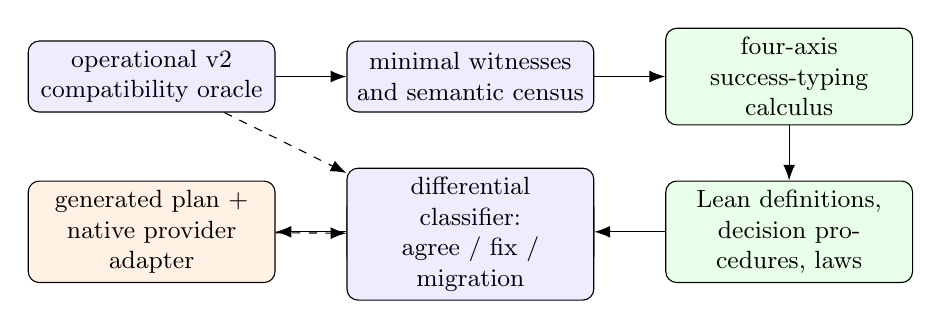
\begin{tikzpicture}[
  node distance=7mm and 9mm,
  box/.style={draw, rounded corners, align=center, minimum height=9mm,
              text width=29mm, font=\small},
  live/.style={box, fill=blue!7},
  proof/.style={box, fill=green!9},
  exec/.style={box, fill=orange!10},
  every edge/.style={draw, -{Latex[length=2mm]}}
]
\node[live] (oracle) {operational v2\\compatibility oracle};
\node[live, right=of oracle] (census) {minimal witnesses\\and semantic census};
\node[proof, right=of census] (axes) {four-axis\\success-typing calculus};
\node[proof, below=of axes] (lean) {Lean definitions,\\decision procedures, laws};
\node[exec, left=of lean] (langdef) {ordered v3\\LanguageDef rules};
\node[exec, left=of langdef] (native) {generated plan $+$\\native provider adapter};
\node[live, below=of census] (diff) {differential classifier:\\agree / fix / migration};
\path (oracle) edge (census)
      (census) edge (axes)
      (axes) edge (lean)
      (lean) edge (langdef)
      (langdef) edge (native)
      (oracle) edge[dashed] (diff)
      (native) edge[dashed] (diff);
\end{tikzpicture}
\caption{Distillation, not cloning.  The compatibility checker supplies
observations; the v3 implementation is generated from a factored calculus.
V2 is never used as a v3 fact interface: the two meet only at a compatibility
or differential boundary.}
\label{fig:petta-typecheck-distillation}
\end{figure}

The four axes are:

\begin{center}
\begin{tabular}{p{.19\linewidth}p{.34\linewidth}p{.37\linewidth}}
\toprule
Axis & Native object & Governing distinction \\
\midrule
Shape compatibility
  & directional consistency on primitive, list, product, union, arrow,
    alias, and nominal-newtype shapes
  & an actual union is universal; a required union is existential; unknown
    is compatible ignorance, not a proof of equality \\
Result cardinality
  & the grade order $\mathsf{det}\leq\mathsf{semidet}\leq\mathsf{nondet}$
    and grade sequencing
  & a deterministic promise cannot be discharged by a computation that may
    fail or branch; effect variables remain polymorphic \\
Stage evidence
  & held, evaluated, and compiled evidence, with an explicit grounding
    license
  & quoted code does not masquerade as its executed value; grounding requires
    compiled-stage evidence \\
Open-world knowledge
  & unknown, empty, or positively typed result evidence, plus selector facts
  & ignorance yields \emph{undetermined}; exhaustion yields
    \emph{incomplete}; only a replayable conflict yields \emph{refuted} \\
\bottomrule
\end{tabular}
\end{center}

The first row explains an initially surprising polarity law.  If a value is
known to be a \code{Number}, a requirement of
\code{(| Number String)} is satisfied by one member.  If the value itself may
be either \code{Number} or \code{String}, a \code{Number}-only requirement is
unsafe because \emph{every} actual alternative must be admissible.  Thus
consistency is deliberately directional and, in the presence of unknown
information, deliberately non-transitive.

\paragraph{A source-level example.}
The following selector is total on proper lists.  The identity
\code{let*} and its administrative alias must preserve both the
\code{List Number} shape and the deterministic grade:

\begin{lstlisting}
(: keep-number (-[det]-> Number Number))
(= (keep-number $x) $x)

(: select-list
   (-[$effect]-> (List Number)
                 (-[$effect]-> Number Number)
                 Number))
(= (select-list () $k) ($k 0))
(= (select-list (cons $head $tail) $k) ($k $head))

(: caller (-[det]-> Number))
(= (caller)
   (select-list
      (let* (($source (cons 1 ()))
             ($items  $source))
        $items)
      keep-number))
\end{lstlisting}

v3 accepts \code{caller}: lexical names elaborate to de Bruijn indices,
alias resolution transports the original runtime evidence, and the selector
consumes the positive proper-list fact.  Replacing
\code{(cons 1 ())} by \code{1} is the negative mirror: the alias still
transports evidence exactly, so the call is rejected at the named shape
boundary rather than accidentally acquiring a list fact.  Replacing the
producer by a nondeterministic superposition of Booleans similarly preserves
shape but fails a deterministic cardinality promise.  These paired examples
ensure that ``transport'' means preservation, not widening.

Stage evidence supplies a second compact example:

\begin{lstlisting}
(: Count (Newtype Number))

(: held-count (-[det]-> Count))
(= (held-count) (quote (brand Count 1)))      ; rejected: held code

(: evaluated-count (-[det]-> Count))
(= (evaluated-count)
   (eval (quote (brand Count 1))))            ; accepted: reactivated
\end{lstlisting}

Quotation preserves latent evidence but does not expose it as runtime typing
evidence.  Only the explicit \code{eval} transition reactivates it.  Native
v3 therefore rejects \code{held-count} and establishes
\code{evaluated-count}; the latter is recorded as a named refinement and
continues to follow v2 until that refinement is explicitly promoted.  This is
why the calculus can make the historical source-grounding defect
unrepresentable: source shape alone cannot construct a grounding license.

\paragraph{Runtime authority and status.}
The executable checker sees program state through exactly five
revision-keyed fact interfaces:
\begin{lstlisting}
EnvDeclared              EnvDeclaredList
EnvNonNewtype            KnownExpressionEffect
KnownExpressionResultType
\end{lstlisting}
They derive facts from the live \PeTTa{} program; they do not call v2 to
manufacture v3 answers.

\begin{figure}[ht]
\centering
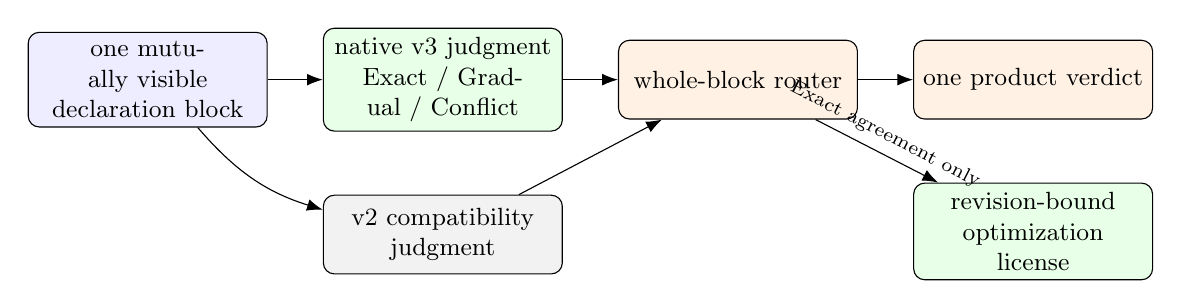
\begin{tikzpicture}[
  node distance=8mm and 7mm,
  box/.style={draw, rounded corners, align=center, minimum height=10mm,
              text width=28mm, font=\small},
  every edge/.style={draw, -{Latex[length=2mm]}}
]
\node[box, fill=blue!7] (block) {one mutually visible\\declaration block};
\node[box, fill=green!9, right=of block] (native) {native v3 judgment\\Exact / Gradual / Conflict};
\node[box, fill=gray!10, below=of native] (legacy) {v2 compatibility\\judgment};
\node[box, fill=orange!10, right=of native] (router) {whole-block router};
\node[box, fill=orange!10, right=of router] (verdict) {one product verdict};
\node[box, fill=green!9, below=of verdict] (license) {revision-bound\\optimization license};
\path (block) edge (native)
      (block) edge[bend right=16] (legacy)
      (native) edge (router)
      (legacy) edge (router)
      (router) edge (verdict)
      (router) edge node[above,sloped,font=\scriptsize]{Exact agreement only} (license);
\end{tikzpicture}
\caption{The KISS compatibility waist.  Routing is per complete block, so a
recursive definition group never mixes authorities.  A gradual result,
conflict, unpromoted refinement, or legacy route cannot mint an optimization
license.}
\label{fig:petta-typecheck-authority}
\end{figure}

At the same 2026-08-14 snapshot, the Lean core contains the executable
sound-and-complete consistency decision procedure, the cardinality and stage
algebras, lexical evidence transport, products, aliases, rational-tree
boundedness, and the Exact/Gradual/Conflict seam, with no holes.  Its ordered
LanguageDef mirror contains 149 rules (134 core and 15 seam rules) and passes
three order/multiplicity mutation canaries.  The isolated native harness
passes 353/353 checks, including product canaries that distinguish exact
agreement from rejection and gradual fallback.  All 51 census-selected
source candidates are executable end to end.  In particular, v3 derives
undeclared result/effect
contracts from the revision-keyed live equation set, retains heterogeneous
results as precise unions, and distinguishes proved concrete selection from
unresolved open patterns.

The complete 389-case differential classifies 214 cases as native agreement,
four as named refinements, and 171 as whole-block legacy-v2, with zero
unclassified, incomplete, or faulted cases.  Current-upstream PeTTaChainer
qualification passes all three representative programs after small,
semantics-preserving migrations that replace effect-polymorphic traversal
helpers with explicit typed recursion.  The no-typecheck profile and v3 both
match the PeTTa reference on those programs.

The optional v3 profile is not yet free.  Three matched runs on the same
materialized programs give the following medians; v3 includes both admission
and ordinary execution:

\begin{center}
\begin{tabular}{lrrrr}
\toprule
Program & no typing & typecheck-v3 & wall ratio & RSS ratio \\
\midrule
\code{deductionrevision} & 1.49\,s & 4.59\,s & 3.08$\times$ & 2.41$\times$ \\
\code{flyingraven}       & 6.07\,s & 12.10\,s & 1.99$\times$ & 1.59$\times$ \\
\code{raveninduction}    & 1.97\,s & 5.26\,s & 2.67$\times$ & 1.98$\times$ \\
\bottomrule
\end{tabular}
\end{center}

This is an integration baseline, not an optimization claim.  Typed fast paths
remain disabled until an exact, current license is consumed at an appropriate
construction boundary.  These denominators are intentionally separate:
operational compatibility, theory/LanguageDef parity, native coverage,
product migration, and execution cost are different claims.

\subsection{Oracle Conformance}
\label{sec:conformance}

For \code{he-compat}, upstream \HE{}~v0.2.10 is the sole oracle, and
the harness is a fail-by-default gate, not a green-manufacturing
report.  Comparison is by \emph{result-bag equality}---multisets of
parsed results, never byte-equality of output text---so formatting
differences cannot masquerade as semantic agreement, and duplicate
results (which are semantically real in MeTTa) are counted.

\begin{description}
\item[Current \HE{} I/O semantic gate.] The per-build oracle gate
  (\code{make test-he-compat-semantic-suite}) replays 23 curated
  \HE{} I/O fixtures against the upstream \HE{}~v0.2.10 baseline.  The
  July~2 receipt reports 23/23 \CeTTa{} passes, 0 failures, and a
  passing baseline check.  Six of those fixtures are core anchors into
  the Lean-side HE I/O conformance file.  This is the current
  conformance claim used by the paper.
\item[Archived catalog material.] Earlier generated rule-capacity and
  broad-corpus catalogs remain useful triage artifacts, but they are not
  treated as current paper evidence unless their driver emits the claimed
  counts on the audited tree.  In particular, this paper does not
  carry a 24-capacity maturity table or a broad-corpus count as a live
  conformance result.
\item[Adjudicated divergences.] Where \CeTTa{} deliberately diverges
  from upstream, each case carries independent grounds.  Three
  examples: upstream's post-0.2.10 \code{function}/\code{NoReturn}
  behavior contradicts its own written specification (a deliberate
  loop fix that left the document stale); upstream's \code{get-doc}
  errors on \HE{}'s own documentation example (an arity regression);
  and the user-visible result of top-level \code{eval} on a
  non-reducible term is genuinely under-determined by the
  specification---both engines deviate from the literal
  instruction-layer reading, in opposite directions.
\end{description}

Conformance is \emph{testing}, and the specification is what gets
\emph{proven about} in Lean: a per-run check is never presented as a
proof.  Where the runtime does emit evidence (the Prime need trace, the
commit traces of the interaction kernel, the receipts of the rho cost
profile), an independent checker replays it; the runtime's own record is
never the authority.

\subsection{Plain \PeTTa{}: Semantic Decisions}
\label{sec:petta-decisions}

For plain \PeTTa{}, SWI-\PeTTa{} at a pinned revision is the oracle, and
comparison is again by result bags.  Where SWI-\PeTTa{} is not consistent
with itself, \CeTTa{} follows the principle its consistent cases express,
not each exception.  Every deliberate departure is an executable entry of
\code{tests/petta/swi\_differences.metta} in the \CeTTa{} repository: the
query, SWI-\PeTTa{}'s answer, the reason and the date of the decision, with
\CeTTa{}'s answers pinned and checked on both execution routes.  The file
records the known departures; finding an unknown one still takes running
both engines.

\begin{description}
\item[Special forms reached at run time.] A special form is syntax only
  where it is written.  Reached at run time---as the value of a variable
  or expression head, as the application a \code{reduce} dispatches, or as
  a function passed to another---its arguments are evaluated first, and
  the application is data unless \PeTTa{} or the program defines a
  function of that name, which is then applied to the values.  This is
  SWI-\PeTTa{}'s \code{reduce/2} rule.  Reading such a value as syntax,
  as \CeTTa{} once did, let a specialization change a program's meaning
  once it learned which form a variable held.
\item[Functions named like forms.] A program may define equations under a
  special form's name.  Where the form is written it keeps its meaning.
  Reached at run time, the name is the program's function, applied like
  any other: at the arity of an equation its equations run, with fewer
  arguments it waits for the rest, and with more it is over-applied.  The
  form never runs in its place, and a call whose equations all fail
  fails rather than becoming data.  Both engines agree.  The two roles
  must stay distinct: a representation that erases the difference
  between the written form and the function cannot keep both meanings,
  and specializing a known name never turns a call into binding syntax
  (\code{PeTTa.BindingForms} and \code{BindingDispatch}, proved in Lean).
\item[\code{let} and \code{let*} reached at run time,] when the program
  defines no function of that name, are data, as \code{if}, \code{case}
  and \code{quote} are in both engines.  The binding form is recognized
  only where it is written: an application reached at run time is not
  binding syntax, whatever its head is named.  Evaluating the data later
  reads it as the syntax it spells, and so runs the binding.
  SWI-\PeTTa{} registers both names as functions without defining one, so
  it returns a partial application, which \code{eval} leaves unchanged and
  which only a \code{let} equation with more parameters, defined later,
  completes.  Decided 2026-09-26.
\item[Errors.] In plain \PeTTa{} an error propagates to the nearest
  \code{catch}, which makes it an \code{(Error \ldots)} value; uncaught, it
  ends the run.  (Prime carries a fault as an occurrence of the outcome
  bag instead, never ending the run; see principle B.11 of the Prime
  specification in the appendix.)  An
  \code{(Error \ldots)} value that a function returns is ordinary data.  A
  run-time dispatch recovers an error raised by the body it runs: that
  path fails, and every other alternative and every answer already given
  remain.  SWI-\PeTTa{} instead discards the body's remaining
  alternatives, so its answers depend on the search order.  Errors in
  argument evaluation, in setting up the dispatch and in over-application
  are not the body's, and propagate.  Specialization keeps the recovery
  of a call that was dynamic where it was written; SWI-\PeTTa{}'s
  specializer drops it (\PeTTa{} issue~223).  For pure, completely explored
  alternatives the recovery distributes over choice,
  $\mathit{handle}(P \cup Q) = \mathit{handle}(P) \cup
  \mathit{handle}(Q)$ on occurrence bags, which is proved in Lean
  (\code{PeTTa.DispatchErrorScope}); so is the check that lets a
  specialization call a callee directly when it raises nothing
  (\code{PeTTa.RaiseFree}).  Decided 2026-09-26.
\item[Over-application.] An application with more arguments than any
  equation of its head takes raises a domain error naming the arities the
  head has, as in SWI-\PeTTa{}: written, dispatched at run time, under
  \code{reduce}, \code{foldl-atom} or \code{collapse}.  Inside the body a
  run-time dispatch runs, it is that body's error and the dispatch
  recovers it.  \CeTTa{} used to return the error as a value and
  continue, contrary to the rule above.
\item[\code{eval} and \code{reduce}] never evaluate a computed result
  again.  \code{eval} evaluates its argument once; \code{reduce}
  evaluates the arguments of the application written in it and
  dispatches the head on their values, as SWI-\PeTTa{}'s \code{eval/2}
  and \code{reduce/2} do.
\item[Imports invalidate specializations.] A specialized function sees
  equations imported after it was specialized; SWI-\PeTTa{} keeps the
  stale specialization.  Decided 2026-09-26, as the meaning of the
  unspecialized program.
\end{description}

\subsection{Evaluator Bug Classes the Campaign Exposed}
\label{sec:bugclasses}

Three bug classes were found and fixed, all instructive.

\paragraph{The Empty algebra.}  When overlapping equations yield a
branch that reduces to \code{Empty}, two dual defects appeared: the
surviving sibling branch was returned without being re-driven to
applicative normal form (violating the spec's applicative order), and
in other shapes \code{Empty} itself leaked into the visible result bag
(the spec is explicit that \code{Empty} ``is not returned among other
results'').  The fix treats the evaluator's outcome set as an algebra
with \code{Empty} as its absorbing zero and re-drives surviving
branches independently of their siblings.  In modal terms
(Section~\ref{sec:modal}): the successor algebra must satisfy
$\Diamond\bot = \bot$.

\paragraph{The one-step congruence bug.}  The reflective one-step
layer reported \code{(+ 1 (+ 2 3))} as a \emph{normal form}: the
one-step relation lacked argument congruence (stepping a reducible
argument when the head cannot fire), while the big-step evaluator had
it.  Because the one-step relation and the evaluator were separately
hand-maintained C branch sets, the gap replicated identically across
three development branches and was invisible to every test that only
exercised head-reducible terms.  The bug was diagnosed through the
modal layer itself ($\Box\bot$ holding on a reducible term), fixed
as deterministic left-to-right congruence matching the evaluator's
applicative order---and is the direct motivation for the rule-pack
weld in Section~\ref{sec:langdefpack}.

\paragraph{The switch/switch-minimal conflation.}  Upstream \HE{}
types \code{switch} as \code{(-> \%Undefined\% Expression
\%Undefined\%)}---the scrutinee is \emph{evaluated} before
matching---while \code{switch-minimal} is \code{(-> Atom Expression
Atom)}, matching the raw scrutinee structurally.  \CeTTa{} routed both
spellings through one structural handler, so
\code{(switch (+ 1 2) ((3 three) ((\$x \$y) (got \$x \$y))))} returned
\code{(got 1 2)} where upstream returns \code{three}.  The defect was
exposed not by testing but by the certification campaign
(Section~\ref{sec:rulecert}): modeling the rules in Lean forced a
precise reading of the two upstream type contracts, and an oracle
probe confirmed the divergence.  The fix splits the rule into
\code{HES\_Switch} (evaluated scrutinee) and \code{HES\_SwitchMinimal}
(structural), with a distinguishing witness pair pinned in the test
suite.

\paragraph{A representative conformance probe.}
The defect classes above are locked by gates rather than by a standing
program suite (standing suites tax every future run; the classes are
the durable artifact).  One representative probe is worth stating
because its \emph{correct} answer is doubly instructive:

\begin{verbatim}
(= (same $x $x) hit)
!(same a a)   ; [hit]
!(same a b)   ; [(same a b)]  -- inert, NOT hit, NOT empty
\end{verbatim}

\noindent
A nonlinear pattern constrains both positions to be equal, so
positional pattern compilation without an equality check answers
\code{hit} --- and an engine grounded in a failure-driven host answers
with an empty bag --- while the specified behaviour is that the
unmatched call remains \emph{uninterpreted}.  \CeTTa{}'s eager and lazy
lanes and upstream \HE{} agree on this and on the sibling probes for
grounded-argument strictness, duplicate multiplicity, view
invalidation, and strict equality; engines with different declared
semantics (\PeTTa{}'s Prolog grounding, set-carrier stores) simply
answer as their own specifications say, which is what declared
contracts are for.

\subsection{Checker Bug Classes the Native Authority Flip Exposed}
\label{sec:checkerbugs}

The differential discipline of Section~\ref{sec:bugclasses} was built to
catch \emph{evaluator} defects.  When the \code{prime} lane's conversion
judgment was migrated from its legacy route---normalize both sides
through the \HE{} type-level normalizer, then compare the results
syntactically---to a native $\lambda\Pi$ kernel that decides conversion
directly for the closed, well-scoped fragment, the same discipline exposed
a subtler class: \emph{checker} false negatives.  The migration kept the
legacy route alive as a separately compiled test-only oracle (production
has no toggle back) and compared the two over a pinned eleven-row corpus.
At the corpus's first commit, on 24 August 2026, the routes agreed on six
rows, including the refutation of the unequal well-typed operands
\code{u0} and \code{(-> u0 u0)}.  On two rows the legacy verdict was wrong,
and on three it answered where no answer was licensed:

\begin{verbatim}
!(type:eq (-> (x : u0) u0) (-> (y : u0) u0))
; native: [True]     legacy: [False]
!(type:eq (sigma (x : u0) u0) (sigma (y : u0) u0))
; native: [True]     legacy: [False]
!(type:eq (idx 0) (idx 0))      ; an open, ill-typed operand
; native: unresolved (the query stays inert)     legacy: [True]
\end{verbatim}

\noindent
The first two pairs differ only in the name of a bound variable.  The legacy
route compared names where it should have compared binders, and so
\emph{refuted} a true conversion.  The instructive part is not that a
procedure was incomplete---that is ordinary---but that its incompleteness
was silently promoted to refutation authority.  An incomplete procedure can
honestly answer ``incomplete''; it cannot honestly answer ``no.''

Three consequences are locked into the gates.  First, verdict equality
with a buggy oracle cannot be the acceptance criterion for a checker
migration.  The current gate states the separation exactly: without the
kernel only the built-in numeric constants are decided; the kernel alone
decides the six universe and binder comparisons; ill-typed operands stay
unresolved on both routes.  The pinned expectation files keep the
divergence as a permanent witness rather than a silent fix---the same
adjudication policy Section~\ref{sec:conformance} applies to upstream
behavioral divergences, now applied to a typing judgment.  Second, the
repaired class must earn its authority: mutation canaries that corrupt the
kernel's admission (the receipts and generations of checking and of
synthesis) are killed by the suite, so the tests demonstrably constrain the
code that produces the new verdicts.  Third, the flip is class-exact and
fail-open: outside the recognized fragment nothing is refuted, and
exhausting the native budget reports incomplete rather than silently
retrying the other authority---a verdict must never depend on which
checker happened to have budget.  The four files of the closed
$\lambda\Pi$ corpus (conversion, checking, synthesis and formation) give
their expected outputs on the draft binary of Appendix~\ref{app:runs}.

The same lesson closed a sibling defect at the interaction of typing
and matching: a typed-applicability pruning path refuted
candidate pairs that the positive matcher accepts (a space-class
mismatch between a negative license and the positive semantics it
claims to approximate).  The rule that covers both incidents: a
negative answer is a claim about all executions, and may only be issued
by an authority whose completeness for that claim is established;
everything weaker prunes nothing and abstains.

\subsection{The Reflective Modal Layer}
\label{sec:modal}

The library \code{lts} (generic, step-parameterized) and
\code{lts:he} (bound to the \HE{} evaluator's one-step relation) reflect the
one-step reduction relation into MeTTa as data:

\begin{itemize}
\item \code{lts:he:transitions} emits the one-step successor set
  of an atom as quoted states (zero results on quiescent atoms);
  \code{lts:he:trace-2} enumerates two-step traces.
\item \code{lts:he:is-normal-form} is exactly $\Box\bot$ (every
  successor satisfies falsity, i.e.\ no successor exists);
  \code{lts:he:is-can-step} is $\Diamond\top$.
\item \code{lts:he:box}~$\phi$ and \code{lts:he:diamond}~$\phi$
  generalize these to arbitrary unary predicates: $\Box\phi$ holds
  when every one-step successor satisfies $\phi$ (vacuously at normal
  forms), $\Diamond\phi$ when some successor does.
\end{itemize}

The De~Morgan law $\Box\phi = \lnot\Diamond\lnot\phi$ is installed as
a runtime self-test; it is the executable mirror of the Galois
connection proven once and for all in the Mettapedia OSLF framework,
where $\mathrm{LanguageDef}\to\mathrm{RewriteSystem}\to
\mathrm{ReductionSpan}\to(\Diamond,\Box)$ is derived generically and
\code{langGalois} establishes the adjunction.  Native behavioral types
in the sense of Native Type Theory arise as predicates over exactly
this reduction span; the runtime implementation and the Lean derivation
describe the same object at two levels.

Multiplicity discipline: \code{transitions} preserves the result
\emph{bag} (duplicate successors are semantically real), while the
modal predicates quotient to reachability.  Evaluation and conformance
compare bags; $\Diamond/\Box$ use support.  Result sets are never
deduplicated for speed.

\subsection{The Small-Step Rule Table}
\label{sec:langdefpack}

The congruence bug demonstrated the structural disease: reduction
rules as anonymous, duplicated C branches are invisible, unremovable,
and untestable-by-absence.  The cure is to make the rule set a
\emph{named, reflectable object} the evaluator provably depends on.

Three granularity strata are kept distinct.  \emph{HEFine} is the Lean
\code{mettaHE} instruction machine (59 rules over interpreter states;
the proof reference).  \emph{HE small-step} is the coarse user-visible
one-step relation---one observable source rewrite, e.g.\
\code{(+ 1 (+ 2 3))} $\to$ \code{(+ 1 5)}---which is what the
\code{lts} layer exposes.  \emph{HEBigStep} is full evaluation.  The
table encodes the small-step relation; its relationship to the fine machine is a
collapse/simulation with explicit provenance links (each coarse rule
names the fine rules that justify it), never a label identity.

The runtime object, \code{CettaLangDefPack}, carries: language,
profile, and granularity identifiers; a schema version; a source
digest over the canonical rule-descriptor text; the rule table; a
disabled-rule mask populated from the
\code{CETTA\_LANGDEF\_DISABLED\_RULES} environment variable; and a
\emph{per-rule claim level} recording the strongest evidence behind
each rule (Section~\ref{sec:rulecert}).  The table has seventeen rows.  Ten rule classes are live and
gate the \emph{only} implementations of their behavior in the one-step
subsystem: grounded dispatch, leftmost expression congruence, equation
match, \code{eval}, \code{chain}, \code{let}, \code{let*},
\code{case}, \code{switch}, and \code{switch-minimal} (the last two
split per their distinct upstream contracts,
Section~\ref{sec:bugclasses}).  Seven rows are accounted but not
gateable.  Four are quiescence rows (quote, return, empty and error),
since disabling them would make the semantics incoherent rather than
smaller.  Three record full-evaluator behaviour of the extended profile
that is not a coarse one-step rule: a comma in a space position folds
the pointwise bag meet of the spaces, a pipe their additive union, and a
two-argument sourced \code{match} is a seed-threaded conjunction across
named spaces.  Each row carries a
provenance string naming the fine-machine rules that justify it.  The
pack is reflected into MeTTa by \code{lts:he:step-rules}.

The load-bearing test is \emph{anti-decorative}: a dedicated lane
re-runs the witness suite with each live rule disabled and
\emph{requires} the witnesses to fail (the successor set must go
empty; normal-form must flip)---baseline plus ten rule-removal
failures confirmed.  If the witnesses still passed with a rule
removed, a duplicate hidden code path would exist---precisely the
disease that produced the congruence bug.  A disabled special form
goes \emph{inert} (its head stays uninterpreted; congruence still
applies), per the principle that unknown symbols are data, never
errors.  The lane fails closed in both directions and runs on both the
default and MORK-bridge builds.

Claim levels are deliberately \emph{excluded} from the digest: the
digest fingerprints rule \emph{content} (names, profiles, provenance,
schema), while claims are \emph{evidence about} that content.
Upgrading a rule's certification therefore must not---and verifiably
does not---move the semantic object: the digest
stays fixed across claim flips; it moves only when rule content
changes.  At the pre-main binary of Appendix~\ref{app:runs} it is
\code{fnv1a64:eda58fb31fa185e1}, schema~2.  The pack is, by design, a hand-maintained
object kept honest by the removal lane and the digest; we deliberately
parked an earlier plan to generate specialized C from the rule source,
because the weld's value lies in the named semantic object and its
fail-closed tests, and code generation is machinery the certification
program does not need.

\subsection{Lean Certification of the Rule Table}
\label{sec:rulecert}

Each per-rule claim takes one of three values, in increasing strength:
\emph{bag-tested-adequate} (the rule's behavior matches the legacy
path and oracle bags on the witness corpus),
\emph{rule-sound-on-fragment} (a compiled, sorry-free Lean theorem
proves the rule absorbed by the official declarative semantics on an
explicitly characterized fragment), and \emph{rule-sound} (the same,
unconditionally).  A claim flips only when the compiled theorem
exists, so the reflective layer can never overclaim.  The
certification route is \emph{absorption}: for each coarse rule, a
theorem that whenever the rule relates $a \to a'$, the official
declarative judgment of the Mettapedia \HE{} formalization
(\code{MettaCall}, \code{MinimalStep}, or \code{EvalAtom}) already
relates the same atoms.  Five of the ten live rules carry
certification; the claims below are those the pre-main binary reports
through \code{lts:he:step-rules}:

\begin{center}\footnotesize
\begin{tabular}{lll}
\toprule
rule & claim & Lean witness \\
\midrule
\code{HES\_GroundedDispatch} & rule-sound-on-fragment &
  \code{mettaCall\_absorbs\_grounded\_dispatch} \\
\code{HES\_EquationMatch} & rule-sound &
  \code{mettaCall\_absorbs\_equation\_match} \\
\code{HES\_Eval} & rule-sound &
  \code{minimalStep\_absorbs\_eval} \\
\code{HES\_Chain} & rule-sound-on-fragment &
  \code{minimalStep\_absorbs\_chain\_source}/\code{\_subst} \\
\code{HES\_LeftmostExprCongruence} & rule-sound-on-fragment &
  \code{evalAtom\_absorbs\_congruence\_frag} \\
\code{HES\_Let}, \code{LetStar}, \code{Case}, & bag-tested-adequate &
  in progress \\
\quad\code{Switch}, \code{SwitchMinimal} & & \\
\bottomrule
\end{tabular}
\end{center}

The certified fragment for the congruence and chain rules is
characterized positively: untyped constructor-headed expressions with
quiescent spectator arguments and a grounded-dispatch or
equation-match redex.  Its supporting theory is a short ladder of
compiled lemmas: a quiescence domain on which atoms officially
self-evaluate, uniqueness of that self-evaluation, transport of
official evaluation across a single changed argument, and absorption
of inner fragment steps---about which the honest surprises accumulated
(e.g.\ a bare \code{Error} \emph{symbol} at tuple head becomes
error-shaped, so the fragment must exclude it explicitly).

The five remaining rules are upstream \emph{stdlib sugar}: their
one-step behavior is the upstream definition of \code{let},
\code{let*}, \code{case}, \code{switch}, and \code{switch-minimal} as
\code{unify}/\code{chain} programs.  Certifying them required a
\emph{matcher bridge}: relating the public equation-query API to the
official \code{matchAtoms}/\code{mergeBindings} semantics.  The key
insight from this development stage was that the real seam was \emph{not} merely a
direct one-way-to-two-way matcher comparison.  The public \HE{} query
API had historically routed equation lookup through the simplified
\code{simpleMatch} path, while the faithful two-sided matcher already
existed separately.  We therefore split the bridge into three explicit
layers.

First, \code{DeclMatchSpec.lean} states the author's
\code{match\_atoms} semantics declaratively and proves the executable
\code{matchAtoms} helper sound and complete against it
(\code{matchAtoms\_sound}, \code{matchAtoms\_complete}).  Second,
\code{DeclMergeSpec.lean} does the same for
\code{merge\_bindings}/\code{add\_var\_binding}/\code{add\_var\_equality},
proving \code{mergeBindings\_sound} and
\code{mergeBindings\_complete}.  Third,
\code{QueryInterfaceAgreement.lean} proves a bounded adequacy theorem for
the \emph{public} query interface:
\code{queryEquations\_ground\_two\_way\_adequate} and its
\code{queryEquationsAgainstVisible}-companion show that, on the
ground-query fragment and under the explicit freshening adequacy
hypothesis \code{EquationFresheningAdequate}, the repaired
\code{matchAtoms}/\code{mergeBindings} API and the legacy
\code{simpleMatch}-based scan agree in both directions up to replay
fuel.

The earlier singleton-seed factorization theorem remains one ingredient
inside this story, but it is no longer the whole story.  The decisive
insight is the G3/G3b split: equality-threading becomes observable only
when the queried atom itself still contains variables, because that is
the point at which \code{Bindings.resolve}/\code{Bindings.apply} must
honor equalities rather than plain assignments.  We therefore bank the
ground-query adequacy result as the honest current certification
API, and carry the variable-bearing query case as an explicit next
obligation rather than silently pretending the legacy API was already
faithful.

%% ────────────────────────────────────────────────────────────────────
\section{Lines of Development}
\label{sec:lines}

\CeTTa{} is developed on several lines at once, each a git branch with its
own worktree and its own purpose.  This section gives each line's purpose,
what landed and when, and what it measured.  Dates are those of the commits.
Numbers come from the measurement reports written as the work landed; each
says what was measured, against what, and how often.  ``Instructions'' are
user-mode instructions counted by \code{perf}; ``G'' is $10^9$ of them.

\begin{figure}[ht]
\centering
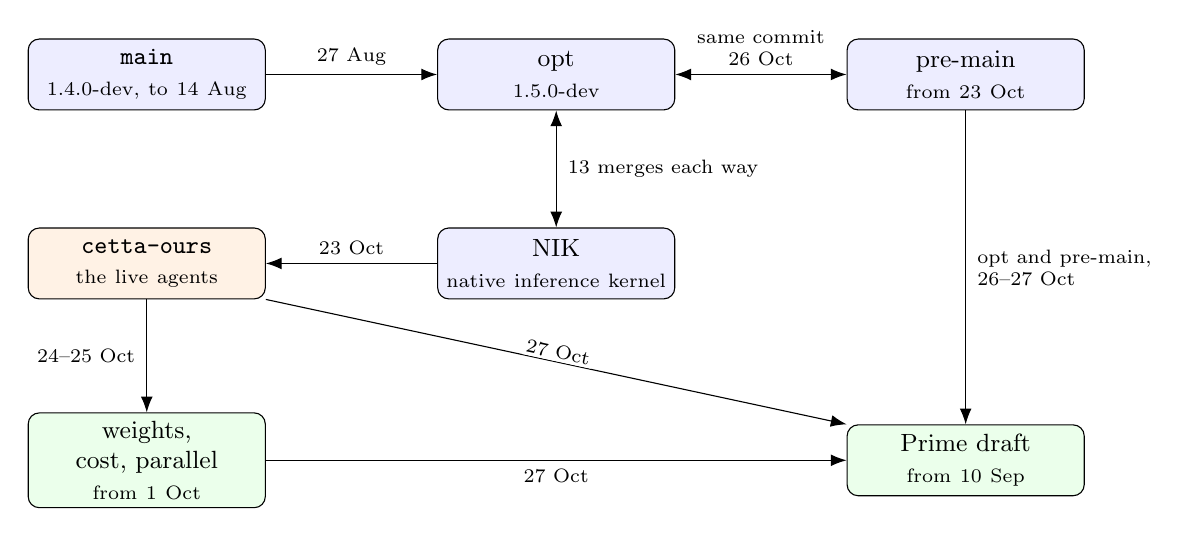
\begin{tikzpicture}[
  line/.style={draw, rounded corners, align=center, font=\small,
    minimum height=9mm, inner sep=3pt, text width=28mm},
  prime/.style={line, fill=green!8},
  main/.style={line, fill=blue!7},
  lab/.style={font=\scriptsize, fill=white, inner sep=1pt},
  >={Latex[length=2mm]}]
\node[main] (main) at (0,0) {\code{main}\\{\scriptsize 1.4.0-dev, to 14 Aug}};
\node[main] (opt) at (5.2,0) {opt\\{\scriptsize 1.5.0-dev}};
\node[main] (pre) at (10.4,0) {pre-main\\{\scriptsize from 23 Oct}};
\node[main] (nik) at (5.2,-2.4) {NIK\\{\scriptsize native inference kernel}};
\node[line, fill=orange!10] (ours) at (0,-2.4) {\code{cetta-ours}\\{\scriptsize the live agents}};
\node[prime] (wts) at (0,-4.9) {weights, cost, parallel\\{\scriptsize from 1 Oct}};
\node[prime] (draft) at (10.4,-4.9) {Prime draft\\{\scriptsize from 10 Sep}};
\draw[->] (main) -- node[lab, above=2pt]{27 Aug} (opt);
\draw[<->] (opt) -- node[lab, above=2pt, align=center]{same commit\\26 Oct} (pre);
\draw[<->] (opt) -- node[lab, right=3pt]{13 merges each way} (nik);
\draw[->] (nik) -- node[lab, above=2pt]{23 Oct} (ours);
\draw[->] (ours) -- node[lab, left=3pt]{24--25 Oct} (wts);
\draw[->] (pre) -- node[lab, right=3pt, align=left]{opt and pre-main,\\26--27 Oct} (draft);
\draw[->] (wts) -- node[lab, below=2pt]{27 Oct} (draft);
\draw[->] (ours.south east) -- node[lab, above, sloped]{27 Oct} (draft.north west);
\end{tikzpicture}
\caption{The lines and their main merges in October.  An arrow points from the
line merged to the line that merged it.  The weights line also took the draft
and pre-main on 24 and 25 October, and the draft had taken opt, NIK, the
weights line and \code{cetta-ours} several times before
(Section~\ref{sec:line-draft}).}
\label{fig:lines}
\end{figure}

\begin{center}
\small
\begin{tabular}{@{}lp{0.20\linewidth}p{0.47\linewidth}@{}}
\toprule
line & head on 27 Oct & purpose \\
\midrule
\code{main} & 12da03b4, 14 Aug & the published, qualified baseline \\
opt & feba78e3 + 59 staged files & the careful fixes: execution, query and memory architecture \\
pre-main & feba78e3 + staged repairs & one execution contract across the machines, qualified for \code{main} \\
NIK & 2f168dca & native inference kernels, then native application libraries \\
Prime draft & a0f1077a + staged basis & Prime in C, in step with its metatheory \\
weights & 750896ae & weights, cost accounting and parallel execution for Prime \\
\code{cetta-ours} & d436e11b & the engine of the live agents, kept running by quick fixes \\
\bottomrule
\end{tabular}
\end{center}

\noindent
A finding on \code{cetta-ours}, where quick fixes keep the agents running, is
a lead for opt to reproduce and root-cause, never a change to copy.  Opt's
method, stated with its October goal, is to find the floor of a cost by
specializing, ask how broad a region of programs the semantics admits, build
the fast path for that whole region, and prove it admissible with executable
laws.

%% ────────────────────────────────────────────────────────────────────
\subsection{\code{main}}
\label{sec:line-main}

\code{main} is the published baseline of the public repository.  Its README
describes it as a direct C runtime for MeTTa whose default lane is the \HE{}
evaluator, and as a working snapshot rather than a polished release.  Its 215
commits run from the first evaluator (19 March 2026) through the
storage substrate (term universe, MORK and \PathMap{} backends, April), \HE{}
conformance and the rho calculus (June), the tail-safe collector (2 July),
Prime, parsing and dependent search (July), to a main-readiness tranche in
August: the native \PeTTa{} corpus at 176/176, the counted-\PathMap{} query
route, \code{MatchDecision}, \code{typecheck-v2}, the Prime outcome carrier
and MeTTa Zero.  The last integration was declared qualified on 11 August, by
a composed exhaustive run of 15 commands taking 7{,}490\,s, with the \PeTTa{}
corpus at 183/183 and \code{fib(999999)} giving the same SHA-256 digest on
the \HE{}, Prime and \PeTTa{} lanes.  The same tranche retired the ground-call
memoization table, which earlier drafts of this paper described.

Nothing has landed on \code{main} since 14 August.  Every other line contains
it: pre-main is 205 commits ahead of it.

%% ────────────────────────────────────────────────────────────────────
\subsection{opt}
\label{sec:line-opt}

The opt line (branch \code{cetta-shared-opt-audit-20260807}) is the
integration base for the execution, query and memory architecture, and the
line of careful fixes.  Its September work is in
Section~\ref{sec:benchmark-programs}; this section covers October.

\paragraph{What landed.}
\begin{center}
\small
\begin{tabular}{@{}lp{0.73\linewidth}@{}}
\toprule
date & what \\
\midrule
1 Oct & conformance checkpoint; an optional durable store; the open tier takes whole sequences \\
3 Oct & the typed tier: compiled \PeTTa{} typed calls reuse exact guard facts \\
4--5 Oct & owned execution: explicit ownership, owned \HE{} and \PeTTa{} sequencing, canonical \HE{} on owned continuation frames shared with \PeTTa{} \\
7 Oct & directional matching (\code{=\%} rules, the \code{pat} library) \\
10--11 Oct & the regional execution core: owned control and return storage, producer dependencies, ordered term-path indexes, counted conjunctions and cursors \\
13 Oct & tabled suffix forwarding, a head-chain store, removal by marks (a bitmap with a Fenwick tree, one contraction per batch) \\
14 Oct & the \PeTTa{} default pinned to version 1.0.6, with version selection \\
16 Oct & resource lifetimes: results moved out of dying storage, ground matches from exact occurrences, reclaimable arena names, suspended calls that keep only what resuming needs \\
17 Oct & HOL Light, MM0 and Megalodon kernels; streaming files; \code{lib\_re}; \PeTTa{} becomes the default language \\
18 Oct & the prepared machine runs typed calls and MeTTa-defined library forms \\
19--20 Oct & 64-bit variable identities; semi-naive saturation; one closure engine \\
20--23 Oct & \PeTTa{} fast regions; JSON, process and tensor libraries merged from NIK \\
24--25 Oct & the evaluator tax: \code{not} and \code{case} in the prepared machine, closures specialized by use (4b74b879), lifting by shape, \code{let} destinations admitted by evidence \\
26 Oct & native \code{transform}, complete \PeTTa{} lists built flat, late output, linear drains and the head index (2030a80f) \\
26--27 Oct & a spread hash for \code{unique-atom} (a93e4a6f); then, staged and not yet committed, bag-order reads, set spaces, a native query path, worst-case-optimal joins and joins over rows of bits \\
\bottomrule
\end{tabular}
\end{center}

\paragraph{The ledger against SWI-\PeTTa{} 1.0.6 (23 October).}  A fixed panel
of 96 cells in 19 families, timed as whole processes, three-run medians,
against the faster of two SWI-\PeTTa{} references (version 1.0.6 upstream and
the local reference checkout on SWI-Prolog 10.1.9).  All 96 matched their
declared observations.  Of the 92 comparable cells, \CeTTa{} was clearly faster
on 78, SWI-\PeTTa{} on 8, and 6 overlapped.  Representative cells:

\begin{center}
\small
\begin{tabular}{@{}lrr@{}}
\toprule
cell & \CeTTa{} & SWI-\PeTTa{} \\
\midrule
HOL benchmark & 1.235\,s & 5.977\,s \\
Peano & 0.017\,s & 1.520\,s \\
MateSpace2 & 0.421\,s & 5.357\,s \\
Nil, 233{,}680 proofs & 1.718\,s, 822.9\,MiB & 15.382\,s, 7{,}416.5\,MiB \\
grouped join and count & 1.134\,s & 11.034\,s \\
selector over 2{,}048 closures (a loss) & 2.04$\times$ SWI & \\
Ambient (overlap) & 15.653\,s & 14.021\,s \\
\bottomrule
\end{tabular}
\end{center}

\noindent
Seven of the eight SWI-\PeTTa{} wins read foreign data, and on those cells
45--60\% of \CeTTa{}'s instructions are in the embedded Prolog engine; on every
other cell but the chainer cells (7--8\%) and one short Nil example dominated
by the engine's start (about 11\,ms), the Prolog share is at most 2.3\%.

\paragraph{Closures (24 October).}  A site applying many distinct closures
paid an analysis per closure.  Specializing a closure from its second call,
and telling values apart within their shape, took the 2{,}048-closure selector
from 0.164\,s to 0.064\,s (SWI-\PeTTa{} 0.114\,s) and a 100{,}000-cell walk
from 0.615\,s to 0.064\,s (SWI-\PeTTa{} 0.264\,s), best of three.  A first
screen missed the chainer cells, which rose by 2--2.4\% in instructions; lifting
closures by shape the next day brought them to 0.85--0.90 of their earlier
count.

\paragraph{The evaluator tax.}  A step of a loop written with \code{case}
cost 26{,}820 instructions against 3{,}854 for the same loop written with
\code{if} and \code{let}, and a step using \code{not} cost 31{,}369, because
those forms fell off the prepared machine into the general one (8{,}004
matches, exact counts, 24 October).  Moving them into the prepared machine
brought a loop called through a caller's \code{case} from 8{,}585 to 3{,}785
instructions per step, with the 97-cell screen unchanged (geometric mean
1.0002).  Measured again on 26 October, integration had reopened the gap:
from a pre-main checkpoint of 25 October the ten gate shapes cost
11{,}470--14{,}080 instructions per element against 3{,}560 before, because
an answer producer deep-copied its data twice; no merge had run the tax gate.
After the repair the shapes cost 3{,}200--5{,}500 per step, and one of the ten
(\code{case} with a byte slice, 5{,}459 to 5{,}694 depending on the build)
remains above its 5{,}000 budget.

\paragraph{\code{transform}, lists and drains (26 October).}  The native
\code{transform} of Section~\ref{sec:tut-transform} fires the library's
rows over the spaces' occurrence cursors and one trail-backed binding
environment, and declines whenever the library or any data constructor it
uses has been redefined, so the authored definition then runs.  A
differential checks native, authored and specification firings on fixed and
seeded programs; an independent check agreed on 1{,}992 of 2{,}018 firings,
the rest being 20 null firings and 6 removals of a bare symbol.  Building
complete \PeTTa{} lists flat, and binding a list built by \code{cons} after
the body, removed most of the library's interpretation cost.  Wall times on a
loaded machine (load about 14 on 16 cores; the report does not state run
counts):

\begin{center}
\small
\begin{tabular}{@{}lrrr@{}}
\toprule
program & native & library on \CeTTa{} & library on SWI-\PeTTa{} \\
\midrule
COMM wave, 400 pairs & 0.020\,s & 0.033\,s & 0.110\,s \\
drain, 1{,}600 jobs & 0.039\,s & 0.064\,s & 0.142\,s \\
drain, 6{,}400 jobs & 0.123\,s & 0.232\,s & 0.330\,s \\
closure, 40 nodes & 0.037\,s & 0.133\,s & 0.207\,s \\
counting, zero groups & 0.016\,s & 0.018\,s & 0.092\,s \\
\bottomrule
\end{tabular}
\end{center}

\noindent
The 6{,}400-job drain peaks at 33\,MB on \CeTTa{} and 60\,MB on
SWI-\PeTTa{}.  Drains had been quadratic for two separate reasons: a
\code{once}-\code{match} built and sorted every remaining candidate, and a
removal settled marks that forced a trie rebuild.  Reading through marks, a
head index per head symbol and length, lazy matches on pinned cursors, and
committing after the proposal unwinds made them linear: in instructions at
1{,}600 and 6{,}400 jobs, native 3.56G and 51.3G became 0.55G and 2.09G, and
the hand-written loop 1.00G and 13.3G became 0.24G and 0.93G.  The
specification library \code{lib\_transform\_specs}, quadratic by design, still
runs 1.8--2.3 times slower than on SWI-\PeTTa{}.

\paragraph{Joins against MORK (27 October, staged).}  The latest opt work is
staged but not committed.  It targets the programs MORK's MM2 language runs
well, against MORK rebuilt from current upstream and SWI-\PeTTa{} running the
faster correct program per task.  MORK and SWI-\PeTTa{} are single runs or
best of two; \CeTTa{} is best of three.

\begin{center}
\small
\begin{tabular}{@{}lrrrr@{}}
\toprule
task & MORK & SWI-\PeTTa{} & \CeTTa{} & \CeTTa{} RSS / MORK \\
\midrule
transitive closure, 50K edges & 1.13\,s & 4.25\,s & 0.167\,s & 1.39 \\
5-clique & 21.2\,s & 18.6\,s & 0.009\,s & 1.80 \\
odd-even sort, 300 & 0.187\,s & 1.27\,s & 0.119\,s & 3.06 \\
backward chaining, 1{,}000 & 15.7\,s & 0.27\,s & 0.026\,s & 1.67 \\
Hexlife, 20 generations & 20.0\,s & 0.15\,s & 0.040\,s & 2.04 \\
ancestry, 1{,}000 & 1.48\,s & 19.0\,s & 0.576\,s & 2.71 \\
reachability, 500 & 8.71\,s & 0.21\,s & 0.035\,s & 0.43 \\
counter machine, 300 & 104\,s & 1.76\,s & 0.544\,s & 0.60 \\
process calculus, 200 & 26.3\,s & 27.9\,s & 8.10\,s & 1.32 \\
\bottomrule
\end{tabular}
\end{center}

\noindent
The odd-even sort's peak memory is just over three times MORK's.  The same
batch found that four catalog cells had drifted 4--9\% slower across earlier
batches, each screened only against its predecessor; screened against the
goal's starting point the catalog is now 4.0\% faster on the geometric mean,
with no cell above $+1.5\%$.

\paragraph{Set aside.}  An earlier broad branch of Nil support was archived on
6 October: building a term could run code and child spaces copied the whole
parent.  A change that returned every \HE{} call's value at once was reverted
on 17 October after it reproduced a duplicate from \code{unique} and let
library natives ignore added equations; its non-\HE{} parts returned the next
day.  An attempt to merge opt into the \code{cetta-ours} and weights
integration was aborted on 17 October (41 conflicted files).

\paragraph{Open.}  The staged work awaits commit.  The committed spread hash
for \code{unique-atom} disagrees with structural equality on two
representations of the empty list, and the checked replacement is not yet
committed.  \code{remove-atom} of a bare symbol answers \code{true} and leaves
the symbol.  Timing holds stand on three cells (+6\% to +14\%).
SWI-\PeTTa{} still wins on Ambient, the rho cell, the chainer cells (2.3--3.8
times) and the foreign-read cells.

%% ────────────────────────────────────────────────────────────────────
\subsection{pre-main}
\label{sec:line-premain}

pre-main (branch \code{pre-main-20261023}) was branched on 23 October from
c632ecd1, the merge of opt into NIK, to make one line ready for \code{main}:
coherent execution, smaller mechanisms, preserved performance.

\paragraph{The problem.}  \CeTTa{} runs \PeTTa{} through several machines:
the ordinary evaluator, the prepared register machine, the open-equation
machine and the search machine, with the \HE{} evaluator beside them.  Each
crossing between them rebuilt facts the caller already knew; a library native
called from the open-equation machine made a host round trip of about
2.4\,$\mu$s; and once one tier declined a caller, the whole callee closure
paid that cost.

\paragraph{The answer.}  One call and return contract, shared by every route:
a borrowed invocation (\code{CettaInvocation}); a tagged outcome that keeps
``declined'' apart from ``ran and gave no answers'', and finished data apart
from pending computation (\code{CettaCallOutcome}); a return cursor that
hands out answers without calling again (\code{CettaCallReturnCursor});
owned sequencing that keeps a producer alive while its child runs and never
replays an accepted answer (\code{CettaOwnedBind}); shared generated plans for
scoped commitment and error handling; and source-fuel accounting by episode,
with per-position debits.  Each step is paired with a Lean model of its
contract.

\paragraph{What it measured.}  Against the frozen c632ecd1 artifact, on a
fixed 96-cell, 19-family panel (paired runs, medians, geometric means), the
staged state of 27 October is 5.2\% lower in wall time, 3.8\% in instructions
and 1.4\% in peak memory.  Pre-main's own work, measured before it merged
opt's closure work on 25 October, was neutral within half a percent, so most
of the step coincides with that merge.  Measured mechanism gains include an 8{,}004-step agent scan from
37.65\,ms and 468.5M instructions to 18.82\,ms and 241.7M, and an
open-equation-machine native call from 2{,}066 host goals to 2.  Correctness
held at every checkpoint: the 471-program corpus in normal and statistics
builds, 1{,}413 differential queries, and focused sanitizer runs.  Against
SWI-\PeTTa{} 1.0.6, on references timed on 23 October, \CeTTa{} is slower on
Ambient (15.06 against 14.02\,s) and the rho cell (3.80 against 2.87\,s), and
faster on the lambda cell (1.11 against 1.29\,s) and a million-element map
(0.416 against 1.664\,s).

\paragraph{Open.}  Everything after feba78e3 is uncommitted, including the
repair of the hash that kept two representations of the empty list apart.
Native step lowering is held back by measured regressions (first 10\% in
wall time on the NIK cell, after a repair 5.8\% on another).  The source grew by about 8{,}400 lines of mechanism
against an aim of shrinking it by a tenth.  The exhaustive \code{main}
qualification has not been run.

%% ────────────────────────────────────────────────────────────────────
\subsection{NIK}
\label{sec:line-nik}

NIK stands for \emph{native inference kernel}.  Its founding offer was: a
user provides a calculus or an interactive theorem prover as a formal system,
and \CeTTa{} provides a disciplined native kernel for it, an
authority-indexed checking service generated from admitted GSLTs that must
not become a second evaluator.

\paragraph{What landed.}  In August: plural checking authorities in Prime and
direct typing authorities (an admitted type cache cut 100{,}000
\code{get-type} queries from 21.5G to 10.2G instructions), then hosting,
LanguageDef-to-ParserPack generation and JSON.  In September:
\code{lib\_tptp} and type interfaces.  From mid-September the line became the
home of native application libraries for the agents and an automated
mathematician port: TPTP and SZS results, JSON values, process execution and
interactive process streams, \code{lib\_re}, tensors, sparse postings and
embeddings, and a persistent connection to a Lean process.  Opt merged NIK
thirteen times and NIK merged opt at least fifteen; merging them on
20 October moved 17 workloads by $+0.74\%$ wall time and $+0.007\%$
instructions (seven trials).  The automated mathematician's 875 supplied
proofs replay through MeTTa and an independent Lean check.

\paragraph{Side branches.}  Three side lines branched from NIK.
\code{nik-vibe-mm0-20261002} holds uncommitted work on kernel formation for
VibeITP and MM0 certificates.  \code{failed/nik-native-he-module-20261008}
archives native \HE{} modules as one commit, never merged.  A detached
worktree holds an Agda checker.

\paragraph{Set aside.}  The native \HE{} modules were correct on every gate but
slower (instructions $+26\%$ on forward chaining, $+109\%$ on an eight-way
join), and were archived on 8 October and restarted one step at a time.  An
Agda checker inside NIK was wound down: it could not refute.  Rebuilding the
MM0 checker in MeTTa on the current tier was judged a loss against the native
checker.

\paragraph{Open.}  NIK's head adds incremental-compression libraries to opt;
93 files of shared learner work are staged.  The kernel-theory programme has
not yet run a kernel with real binders under two-way adequacy, or a measured
computation tier against MM0 or Dedukti.

%% ────────────────────────────────────────────────────────────────────
\section{The Prime Families}
\label{sec:prime-families}

Three lines carry Prime and the agents built on \CeTTa{}: the Prime draft,
the weights, cost and parallel line, and \code{cetta-ours}.  They exchange
work constantly; on 27 October 2026 the draft had absorbed every commit of
the other two.  This section follows them in turn and ends with that night's
merges.  Statements about Prime carry their kind: \kind{draft} for the C
draft's behaviour, \kind{candidate} for a property of a candidate design,
\kind{direction} for a design direction with its reasons, and \kind{decided}
for a recorded decision.

\subsection{The Prime 2.0 draft}
\label{sec:line-draft}

The draft (branch \code{fable-prime-2.0-draft-20260910}) is Prime's one C
worktree.  Its README describes Prime as a higher-order MeTTa in which code is
a value, programs can be checked by a native dependent type kernel, and proofs
are terms the kernel checks, and the draft as the place where Prime's
semantics is settled against its formal metatheory, so its interfaces may
still change.  Its working rule is that everything in Prime has three faces:
extensional (its mathematical meaning, judged in \code{set:} and \code{hol:}
spaces), intensional (how it is built and checked: the \code{type:} language
and the kernel) and operational (what it does when run).  A construct is
finished when it has all three and the links between them: it runs as its
equations say, what runs is typed, and what is typed means the set it should.

\paragraph{What landed.}  The draft's own history is in its branch log rather
than its first-parent chain, because it was fast-forwarded onto
\code{cetta-ours} on 21 October and onto the weights line on 22 and
25 October \kind{draft}.

\begin{center}
\small
\begin{tabular}{@{}lp{0.75\linewidth}@{}}
\toprule
date & what \\
\midrule
10--23 Sep & the worktree begins on opt: \code{lang:}, \code{type:} and \code{set:} judgments with four-valued verdicts, four identity profiles, a curriculum of about 170 judgments; first commit 23 Sep \\
24--29 Sep & the kernel trust boundary and certified transforms; typed conversion with $\eta$; cumulative subtyping; a level-general recursor; theorems published with their context \\
25 Sep--8 Oct & scope machinery: names follow the rho calculus with sealed quotation; own-name records under scope profiles; \code{new} and run-time lambdas; lexical-fresh binding made the default on 8 Oct (115 programs translated, 480 of 480 Lean scope rows matching) \\
1--4 Oct & universe levels below $\varepsilon_0$ with computed written levels; sets ambient; native priority control, demand and resumable search; binary arithmetic and an opt-in native arithmetic oracle; the Megalodon set face quarantined behind an explicit profile \\
12 Oct & a HOL Light guest; declared binding languages; \HE{}-style type declarations answered by the grounded HOL fragments, never by \HE{}'s engine \\
20--23 Oct & a fair first-answer scheduler and its two repairs; data versus \code{Atom} by construction; completed-value producers; one sequence view \\
26 Oct & standard terms redefinable with \code{std:} backups (83cb3038); a mathematical workspace library \\
26--27 Oct & merges of pre-main, opt, weights and \code{cetta-ours}; the interaction kernel, staged \\
\bottomrule
\end{tabular}
\end{center}

\paragraph{Set aside.}  A contextual call-by-push-value lane (1{,}382 lines of
library and its tests) was removed on 22 October to be redone after the
metatheory cleanup.  A tranche of collection space kinds was reviewed as not
mergeable and is not in the tree.  The October loop work was built outside the tree
and has not been ported.  The draft's set face had silently been Megalodon's higher-order Tarski
Grothendieck theory; it was found and quarantined on 4 October.

\paragraph{Measured.}  The draft's measurements are diagnostic rather than
competitive.  Selecting 7 answers under native priority control costs 322
scheduling quanta against 10{,}404 for completing a 200-answer stream (about
6\,ms against 24\,ms).  A \code{let}-body fold over 500 to 2{,}000 items costs
6.5G to 320G instructions, cubic in the length; a native iteration built outside the
tree brought a 1{,}000-item fold from 43.9G to 0.26G but has not landed.
On naive \code{fib 30} the Prime lane takes about 2.6\,s and 271\,MB
against the \HE{} lane's 0.04\,s (single runs, Appendix~\ref{app:runs}): the
need machinery is the cost.

\paragraph{Open.}  Recorded known issues PK-3 to PK-5; thirteen fixtures that
hang or differ because of the weights line (below); \code{==} on state handles
comparing stale contents; the \code{cons}/\code{nil} contract; and the
deviations of Section~\ref{sec:prime-draft}.  Verification of execution
traces and receipts is deferred until the other draft work is resolved.

\subsection{The weights, cost and parallel line}
\label{sec:line-weights}

This line (branch \code{prime-weights-parallel-20261001}, one writer) carries
one goal: graded \code{where} and semantic weights, reflected and certified
costs that programs can inspect, native parallel workers under resource
contracts, and optional history, replay and debugging.  The space service with
multi-account authority grew inside it: generation-stamped grants, stable
service-scoped principals, one-shot tickets and a durable decision ledger.
Its goal requires that fine-grained native execution preserve exact
occurrences, bindings, current authority, declared observations and complete
retained computation.

It was created on 1 October from the draft, integrated owned execution, costs
and parallel control on 11 October, mode-directed workers on 14 October,
optional history on 16 October and native space workers on 18 October, and
took the draft, \code{cetta-ours} and pre-main in three phases on 24 and
25 October.  Its own whole-goal audit of 26 October puts it at about 80\%,
with five of nine gates and 13 of 25 contract families supported, and states
that its earlier estimates of 96\% and 90\% overstated completion; 12 to 20
substantial blocks remain.  Its measured overheads are small where they were
measured: compiled-in history recording costs 0.07--0.18\% in instructions
over 138 executions, and recording on request 5--13\%.  Its first theory
question, what one source interaction observes, keeps, consumes and emits, is
the question Section~\ref{sec:interaction} answers.

\subsection{\code{cetta-ours}}
\label{sec:line-ours}

\code{cetta-ours} (branch \code{cetta-ours} of the \code{godelclaw/CeTTa}
remote) is the engine of the live agents.  Its README describes it as Prime
combined with the native process, timer, mailbox, memory and Telegram
libraries the agents use; the agents pin its revision, and their cognitive
loops run on the \PeTTa{} lane.  It forked from opt on 4 October and has some
200 commits of its own: managed symbols and collection experiments; unified
HTTP, process and channel libraries; a revisioned space service; native
tensors and memory collections with packed cosine search; native mailboxes;
SQLite; authenticated service peers; and the primitives the agents' port from
Python asked for.  It merged opt, NIK, the weights line and the draft
repeatedly.

Its fixes keep the agents running; opt takes its findings as leads.  Three
examples, with the line that root-caused them:

\begin{itemize}
\item A responder grew to 6.7\,GiB over eight hours.  \code{cetta-ours} traced
  it to overlapping library equations and fixed the library (403\,MB to 48\,MB
  on a 1{,}000-cycle probe).  Opt reproduced it on its own head and fixed the
  engine: reclaimable arena names, a resource ledger, and equations guarded by
  \code{decons} leave no alternative behind; the reproducer went from 964.2M to
  332.2M instructions and from 179.2 to 19.1\,MiB.
\item A cut Prolog \code{eval} leaked its state, one per cut.  The quick fix
  disposed of it; opt redesigned the evaluation lifecycle so that a
  three-answer evaluation cut 203 times leaves no state live, and the same
  change designed out a use-after-free.
\item The agents' native ports ran 5 to 30 times slower per step than
  expected.  Opt measured the tax as narrower: the seam between machines,
  where one byte-slice call cost about 25{,}000 instructions as a host goal
  against about 2{,}200 inside the prepared machine
  (Section~\ref{sec:line-opt}).
\end{itemize}

\subsection{The merges of 26--27 October}
\label{sec:merges}

On the night of 26 to 27 October the draft took three merges: opt (as
dd5dbf98, which also brought pre-main), the weights line (as 18c680aa), and
\code{cetta-ours} at d436e11b (as a0f1077a, committed on 27 October).

\begin{itemize}
\item The opt merge kept both atom-table declarations, split cursor admission
  from capture, refused detachment under an owned execution, and carried
  opt's three-argument cursor interface into the draft's own call sites.
\item The weights merge passed 274 of 284 fast Prime fixtures, and did not
  build until one missing argument was supplied in the next merge.
\item The \code{cetta-ours} merge had 22 conflict regions in the space
  service.  The draft's multi-account authority layer and the incoming scoped
  observations now work together: an observation belongs to the principal and
  grant generation that captured it, and an observed batch is journaled with
  its authority stamp and resolved revision.  Journals written by
  \code{cetta-ours} binaries replay in the merged service across a checkpoint.
  Generated files were regenerated from the merged sources, never merged by
  hand.
\end{itemize}

\noindent
The gate after the merges: \code{make test} passes except the manifest check,
which fails on test files of unrelated work in progress and on one fixture
missing from its lane.  In the full Prime gate no failure comes from the
\code{cetta-ours} or opt merges: each also fails on the draft before them.
Thirteen fixtures hang or differ because of the weights line, which fails them
exactly as the merged draft does, while the draft after the opt merge runs
them correctly in under a second.  Their repair belongs to the weights line.

%% ────────────────────────────────────────────────────────────────────
\section{Spaces and Channels: the Interaction Basis}
\label{sec:interaction}

MeTTa has spaces, stores of atoms that programs query and update.  Rholang and
the rho calculus have channels, names on which processes send and receive
messages.  A language for many interacting reasoners needs both, and needs
them to compose: to consult shared knowledge, to consume an obligation exactly
once, to publish a result, to wait, and to do all of it on many processors
without changing what a program means.  A study of 26 October 2026, composed
in~\cite{interaction-basis}, asked what single primitive serves both, what
concurrency it admits, and what language sits on it.  Its answer is the
\emph{direction} this paper adopts for \CeTTa{}'s spaces and channels
\kind{direction}.  This section states the answer, what is proved, what runs
in the Prime draft, and what is missing.

\subsection{One interaction}

A \emph{store} is a finite set of \emph{occurrences}: each occurrence has an
identity that is never reused, and a label saying where it lives and which atom
it carries.  Two occurrences may carry the same atom, so a bag of atoms is a
set of occurrences.  A \emph{commit} is one atomic step with three parts:

\begin{itemize}
\item it \emph{observes}: matched reads pick occurrences, and \emph{predicate
  queries} read a whole region (all of it, a count, or absence);
\item it \emph{disposes}: each matched occurrence is \emph{taken} (consumed) or
  \emph{kept};
\item it \emph{emits}: it \emph{makes} fresh occurrences at any locations.
\end{itemize}

\noindent
A commit is enabled when what it takes and keeps is present, nothing is both
taken and kept, what it makes is fresh, and every predicate query holds.  In the
language of graph rewriting it is a double-pushout span
$L \supseteq K \rightarrow R$ with application conditions: $L$ is what is
matched, $K$ what is kept, $R\setminus K$ what is made, and the predicate queries
are the conditions.  Its four parts, keep, take, make and predicate query, form a
\emph{basis}: none can be encoded by the others relative to a stated observer
(a commit that encodes another must be enabled at the same stores, produce the
same labels, and commute with the same commits).  A fresh name is a kind of
make, not a fifth part, and choice belongs to rules with several rows, not to
the commit~\cite{interaction-basis}.

A predicate query is the part whose answer can change when an atom is
\emph{added}: ``all'', ``how many'', ``none'', and ``everything here is like
this'' (the absence of a counterexample).  Its answer depends on every
occurrence that satisfies its pattern, including one made later, as a predicate
read does in database concurrency control~\cite{predicate-locks}; so it
conflicts with every take or make inside its region.  Each is a fold of the
region's matches through an order-blind operation: \code{all} collects them as a
bag, and a count, absence and uniqueness are folds of that bag.  A matched read
stays true when atoms are added.  This one distinction carries most of the
theory.

\subsection{Spaces and channels are one object}

Four rights, called \emph{facets}, license the four parts at a location:
\code{receive} (take), \code{peek} (keep), \code{send} (make) and
\code{observe} (predicate query).  A commit outside its holder's facets is not
\emph{formed}, and is refused before it runs.  A space is a region whose
holders have all four; a Rholang channel is a region without \code{observe}.
The other named profiles are a mailbox (senders are blind), a log or fact
region (nothing leaves) and a board (readers neither add nor remove).

What makes this more than a naming scheme is that each missing right buys a
law, proved in Lean~\cite{interaction-basis}:

\begin{itemize}
\item where nobody may query a region, arrivals never invalidate anything: a
  commit stays enabled when occurrences arrive outside the regions it queries,
  the cheap per-occurrence claims check is already serializable, and a
  waiting guard is woken only by a make;
\item where nobody takes and nobody queries, replicas merge into a legal
  serial run without coordination, while consuming something exactly once can
  never be coordination free;
\item along runs of formed steps, authority is passed and never created.
\end{itemize}

\noindent
A region's guarantees therefore depend on what \emph{others} may do there, so
its permitted operations are declared with the region, kept by the authority
layer, and checked when a program is formed \kind{direction}.

\subsection{Meta-spaces}

The study's answer to unifying spaces and channels ``into meta-spaces that can
offer different interaction modes'' is a region with independent axes
\kind{direction}:

\begin{center}
\small
\begin{tabular}{@{}lp{0.62\linewidth}@{}}
\toprule
axis & values \\
\midrule
read policy & what ``the same'' means and how answers are read: bag, set, list
  order, or modulo declared equations \\
profile & the facets each holder has \\
predicate-query discipline & owned (one writer), stratified (sealed before the query),
  or shared (validated at commit) \\
coordination policy & free, escrow, owner or lease; home or replicated \\
engine & storage and index; never changes meaning \\
\bottomrule
\end{tabular}
\end{center}

\noindent
Today's dialects become read policies: Prime reads a bag, while \HE{} and
\PeTTa{} read storage order, and a sequence reading specializes a bag reading
but not conversely.  The one constraint between axes the study found runs from
profile to engine: a predicate query modulo equations needs a matcher complete for
those equations.

\subsection{Today's operators as cases of the one form}

\begin{center}
\small
\begin{tabular}{@{}lp{0.62\linewidth}@{}}
\toprule
operator & as one commit \\
\midrule
\code{match} & an \code{every} of a read: one instance per occurrence and per answer \\
\code{add-atom} & a commit that only makes \\
\code{remove-atom} & a take; which occurrences it takes differs by lane \\
counting by \code{collapse} & an \code{all} predicate query \\
\code{unify} & a \code{let} source with no footprint \\
\code{new-space} & a make of a fresh name \\
\bottomrule
\end{tabular}
\end{center}

\noindent
What the form adds is several takes in one commit (atomic joins), predicate
queries with a declared stability discipline, waiting (\code{await}, \code{whenever}),
rights on handles, and installed rules whose installation commutes exactly
with the commits that do not query the rule base.

\subsection{What is proved}

The study produced 106 Lean modules (49{,}762 lines, none with \code{sorry};
every cited theorem uses only \code{propext}, \code{Classical.choice} and
\code{Quot.sound}), covering the commit and its exactness, batches and
\code{every}, traces, isolation modes, waiting and fairness, names and rights,
reflection, a congruent equivalence under which Rholang's receipts are exact
aliases, types (sessions, footprints, facets), clocks and leases, coordination
across locations with its impossibility results, and the admission of rules
promoted from data~\cite{interaction-basis}.  Representative theorems, each
present in the Lean tree: \code{Enabled.frame} (the frame law),
\code{readTake\_one\_refused} (identification), \code{every\_refuses\_clash},
\code{every\_complete\_spoiled\_by\_arrival} and \code{checkRun\_isSome\_iff}
(the trace checker is exact).  A later audit of authority in the Prime runtimes
added a permissions layer of 73 theorems, among them
\code{absence\_preserved\_iff}: a universal read over a region is preserved by
every run of the other subjects exactly when none of them can reach
\code{send} at its names from the initial delegation state.

\subsection{What runs in the Prime draft}

On 27 October 2026 the Prime draft gained a native interaction kernel with a
MeTTa library, five fixtures and a make target, staged for commit
\kind{draft}.  Listing~\ref{lst:t09} runs on it.  Its measured state:

\begin{itemize}
\item \textbf{The commit.} \code{transform} reads, keeps, takes and makes in
  one step across any number of regions; \code{every} rows are linear on their
  own and the whole commit must be linear; predicate queries dispose of nothing; a
  \code{let} runs once its variables are bound.  The kernel matches against the
  live store, checks rights at every read, and never runs code: it hands each
  \code{let} back to the library.
\item \textbf{Regions and handles.} \code{new-region} answers an opaque handle
  sealed by a brand private to the kernel; \code{facet} attenuates it.
  Formation is checked when a firing is formed, when a rule is installed, and
  at run time for locations supplied by data.
\item \textbf{Waiting.} \code{await}, \code{whenever}, \code{choose},
  \code{else}, \code{par} and \code{seq} are implemented; a parked firing is
  woken by any change in a region its last attempt read.
\item \textbf{A corpus in two styles.}  Twelve classic coordination programs
  (producer/consumer, bank transfers, dining philosophers, barriers, reactive
  rules, an MM2-style closure, CHR, Linda, Erlang receive with timeout, Rholang
  contracts, rules as data, leases with fencing) were written twice and run
  under 32 schedules each.  Written with today's idioms (\code{match},
  \code{remove-atom}, \code{add-atom}, counting by \code{collapse}), 11 of the
  12 violate their property under some schedule, though all are correct
  sequentially.  Written with the interaction form, none does.
\item \textbf{Verified traces.} The Lean trace checker accepts all 32 kernel
  traces of the corpus and refuses all 3 corrupted ones.
\end{itemize}

\noindent
Costs were measured on single runs.  Draining 2{,}000 jobs on the Prime lane
takes $4.9\times10^{10}$ user instructions (3.5\,s) with today's idioms,
$1.9\times10^{10}$ (1.4\,s) as a \code{whenever} rule, and $7.4\times10^{9}$
(0.5\,s) as one \code{every} commit, of which filling the queue costs about
$7\times10^{9}$.  On the same task the \PeTTa{} lane runs today's loop in
$1.2\times10^{8}$ instructions, SWI-\PeTTa{} in 0.09\,s, and Rust \HE{} timed
out at 500 jobs and was killed at 15.6\,GB at 2{,}000.  On the Prime lane the
evaluator's need machinery, not the kernel, dominates (61\% of the rule form's
time).

The draft also carries the \PeTTa{}-lane \code{transform} of
Section~\ref{sec:tut-transform}, merged from the opt line.  The two engines
were run on twelve probes whose answers the theorems fix.  The value-level
\PeTTa{} engine deviates on two: it fires a kernel that takes what an
\code{every} row keeps, and it turns two stored schematic atoms into ground
copies.  The occurrence kernel meets all twelve.  The direction is one engine,
the occurrence kernel, with the \PeTTa{} engine's techniques (trail-backed
bindings, \PeTTa{}'s index pattern, presentation admission) moved into it
\kind{direction}.

\subsection{Authority}

An audit on 27 October found that ``authority'' names at least five unrelated
mechanisms in the Prime runtimes \kind{draft}.  Three are permission
mechanisms.  The space service's grant layer (principals, attenuating grants,
one-shot tickets, a durable decision ledger) is unforgeable, attenuating and
revocable, with one escape: a grant's ticket requirement is attenuated by
subset, so a child grant may drop it and append without limit.  The
interaction kernel's region facets are real capabilities with two gaps: a
location that is not a handle resolves to its holder's rights, and one global
seal brand lets a forged board pass.  The evaluator's effect ``authority'' is
a thread-local flag checked against allowlists, which cannot be forged but
cannot be delegated or attenuated either.  The direction is one carrier, the
sealed handles, with the grant table as an instance of the delegation core and
an effect capability in place of the flag \kind{direction}.

\subsection{What is missing}

The native runtime is the gap.  Reading the trees on 26 and 27 October, the
study found no C tree with stable occurrence identities separate from content
identities, per-occurrence claims in canonical order, per-region epochs bumped
by takes and makes, a wait index by guard kind, or persistent receivers that
are kept rather than taken and republished; the draft identifies an occurrence
inside a commit by its space, the space's revision and its position.  The
composed study estimates the native runtime at about 5\% of its scope, the
theory at about 76\% and the surface language at about 50\%.  Three choices
are open: the primary spelling of the firing (the form \code{transform} with
\code{await}, \code{whenever}, \code{choose} and \code{else}, with Rholang's
receipts as aliases, is the current lean), whether \code{Atom} means data, and
which named profiles ship.  The draft's remaining deviations are listed in
Section~\ref{sec:prime-draft}.

%% ────────────────────────────────────────────────────────────────────
\section{MeTTa Prime}
\label{sec:prime}

\code{-{}-lang prime} is a \emph{distinct} MeTTa language sharing \CeTTa{}'s
substrate.  Its ordinary application semantics is branch-local call by need
with call-time choice.  It is not an extension of \HE{}, and does not reduce to
\HE{} by erasure; the ``\HE{} unchanged'' gates that accompany every Prime
change establish that shared code does not interfere, not a semantic
relationship.  Prime is also not one fixed system: it is a web of candidate
type theories with carved profiles, and no statement about ``Prime'' may be
broader than the theorem or behaviour that supports it \kind{decided}.  This
section separates what the C draft does from what is a candidate, a direction
or a recorded decision.

\subsection{Recorded decisions}

The decisions below were recorded with their sources and are not reopened
without new evidence \kind{decided}.

\begin{itemize}
\item \textbf{Identity.} Native identity is intensional, with J and its
  computation rule; K and uniqueness of identity proofs are not global, but
  appear only in explicitly admitted scoped regions or hosted theories; proof
  irrelevance is a mode to switch into, never the default.
\item \textbf{$\eta$.} Prime keeps $\eta$; the known defect, untyped $\eta$
  contraction, is repaired by type-directed $\eta$.
\item \textbf{No fallback to \HE{}'s type engine} (11--12 October).  \HE{}-style
  declarations in Prime are answered by the proper face that grounds their
  fragment; outside it the answer is \emph{undetermined}.
\item \textbf{Sets are ambient, and a type is a set} (2 October).  Which set
  theory sits at the top is under investigation; the Megalodon set theory is
  an opt-in profile, never the default.
\item \textbf{Metavariables denote model elements} modulo the active equational
  theory: a repeated pattern variable means equality modulo that theory.
\item \textbf{Results are unordered multisets.} Order, \code{once} and
  \code{select}, depth-first search, and sharing are opt-in policies; a
  specification fixes no evaluation order.
\end{itemize}

\subsection{The language, as the draft runs it}

\paragraph{Need cells and call-time choice.}  An argument is delayed in a
\emph{need cell}: an opaque runtime capability with an immutable origin and a
checked cache state machine.  Forcing a completed cell replays its cached bag;
completed values and stable faults are memoized, while blackholes and
interruptions remain retryable.  Every use of a cell sees the same value, so
one delayed choice used twice yields correlated outcomes
(Listing~\ref{lst:t03}).  The same distinction is available explicitly:
\code{(let \$p (delay (superpose (A B))) (Pair (force \$p) (force \$p)))}
answers \code{(Pair A A)} and \code{(Pair B B)}, while with \code{resample} in
place of \code{delay} each force chooses afresh and all four pairs appear
\kind{draft}.

\paragraph{Outcomes.}  Prime's computational zero is the absence of
occurrences.  The symbol \code{Empty} is inert data and the empty expression
\code{()} is a unit datum: \code{(collapse Empty)} answers \code{(Empty)}.  A
fault is one occurrence of the outcome bag, beside the others:
\code{(collapse (superpose ((+ 1 1) (car-atom ()) 3)))} answers
\code{(2 (Error (car-atom ()) \ldots) 3)}.  Internally an outcome carries the
ordered occurrence bag, its completion reason and its budget state, so an
incomplete frontier cannot be read as a proof of absence \kind{draft}.

\paragraph{Variables.}  Bare \code{\$} is a fresh anonymous variable at each
occurrence: \code{(= (both \$ \$) yes)} answers \code{yes} for
\code{(both a b)}.  Named variables co-refer: \code{(= (same \$x \$x) hit)}
leaves \code{(same a b)} inert \kind{draft}.  Binding is lexical-fresh by
default since 8 October.

\paragraph{Held data.}  Declare \code{(: hold (-> Atom Atom))},
\code{(: hold2 (-> (Data Atom) Atom))}, and give both the equation
\code{(= (hold \$x) (quoted \$x))} (and likewise for \code{hold2}).  A
parameter typed \code{(Data Atom)} receives its argument as written:
\code{(hold2 (+ 1 2))} answers \code{(quoted (+ 1 2))}.  A parameter typed
\code{Atom} does not hold it: \code{(hold (+ 1 2))} answers
\code{(quoted 3)} \kind{draft}, where the \HE{} lane would pass the
expression unevaluated.  Whether \code{Atom} should mean data is one of the
open choices of Section~\ref{sec:interaction}.

\paragraph{Typing.}  Prime's typing has three faces, linked by the draft's
fixtures: the \code{type:} language and its kernel (intensional), the
\code{set:} and \code{hol:} judgments (extensional), and the evaluator
(operational).  Ordinary function contracts consult the program's selected
\code{get-type} relation, so a program may extend the classifier with its own
equations (Listing~\ref{lst:t07}) without minting a checked theorem: native
theorem publication still checks the proof under its context \kind{draft}.

\paragraph{The standard library is editable.}  Since 26 October standard
definitions are ordinary occurrences of the program space, and
\code{std:}-qualified names keep the originals (Section~\ref{sec:tut-stdlib})
\kind{draft}.

\paragraph{Memoization is opt-in.}  \code{(pragma! search-table-mode variant)}
enables the variant table for the session; with it naive \code{fib 30} takes
about 0.2\,s on the draft's Prime lane (single runs).  Nothing is memoized by
default.  An earlier ground-call table, which an earlier version of this paper
described, was retired from the code on 11 August.

\subsection{Proof search and native kernels}

Prime hosts proof search as type inhabitation over the lazy frontier, with
claim-bearing results lowered to an external checker rather than asserted by
execution.  From August the draft reconstructs ordinary typed constructors at
the ingress of its untrusted rule machine for a strictly positive list
fragment (\code{rel:all}, \code{rel:fold}, \code{rel:list:member},
\code{rel:any}, \code{rel:case-list}), keeping proof-tree shape, intermediate
witnesses and occurrence identity; an unrecognized tree reaches the ordinary
evidence-bearing check instead of being accepted \kind{draft}.  Each
semantic fiber has one target checked across the native kernels; no goal is
routed to a kernel by its feature \kind{decided}.

\subsection{Deviations in the current draft}
\label{sec:prime-draft}

These are behaviours of the draft binary of Appendix~\ref{app:runs} that its
own semantics or recorded decisions say are wrong, each with its reproducer
\kind{draft}.

\begin{enumerate}
\item \textbf{\code{match} ignores outer bindings.}  A variable bound outside
  a \code{match} is fresh inside its pattern (Listing~\ref{lst:t04}).
  \code{transform} respects outer bindings.
\item \textbf{Top-level reads run stored code.}  After
  \code{!(add-atom \&self (stored (add-atom \&self (leaked three))))}, a bare
  top-level \code{!(match \&self (stored \$c) \$c)} runs the stored
  \code{add-atom}; wrapped in an expression, or bound with \code{let}, the same
  read returns data.
\item \textbf{Library loops nest a C frame per item} (known issue PK-3).
  \code{add-atoms} over a \code{let}-bound list of 1{,}340 rows stops with
  \code{(Incomplete stack-exhausted)} after storing 1{,}333 of them; a
  \code{foldl-atom} whose step binds with \code{let} costs instructions cubic
  in its length.
\item \textbf{A streamed fold is quadratic in its answers} (PK-4), and
  \textbf{held values reach sequence operations as a tag and their syntax}
  (PK-5).
\item \textbf{Thirteen fixtures hang or differ} after the weights merge,
  reproduced on the weights line itself (Section~\ref{sec:merges}).
\end{enumerate}

\noindent
Each known issue carries its reproducer, its diagnosis and a repair direction
in the draft's documentation, and is removed by the change that fixes it,
together with a regression test.

%% ────────────────────────────────────────────────────────────────────
\section{Verified \HE{}$\leftrightarrow$\PeTTa{} Translation}

\subsection{Bidirectional Translator}

A bidirectional translator converts between \HE{} and \PeTTa{} dialects.
It is implemented both as relational Prolog
(\code{he\_petta\_relational.pl}, with explicit freshness threading) and
as computable Lean functions (\code{translateHE}, \code{translatePeTTa}).

The translator handles 8 \HE{}$\to$\PeTTa{} rewrite rules
(\code{chain}$\to$\code{let}, \code{collapse-bind}$\to$\code{collapse},
\code{nop}$\to$\code{let~\$fresh~X~()}, etc.)\ and 5
\PeTTa{}$\to$\HE{} rules (\code{progn}$\to$nested \code{let},
\code{prog1}$\to$\code{let} with result capture, etc.).  At its last recorded
corpus run, all 437 \code{.metta} files of the corpus then in use parsed and
translated.

\subsection{The Lean development}

The translation is backed by a Lean development that has grown from two
files to thirteen modules of about 25{,}000 lines.  Its sources
contain no \code{sorry}; every module was built after its last change; and the
two headline theorems audited for this paper use only standard axioms
(\code{simpleMatch\_applyBindings\_comm} uses none,
\code{mettaCall\_equation\_step\_sound} uses \code{propext} and
\code{Quot.sound}).

\begin{description}
\item[Matching correspondence.]
  \code{simpleMatch\_applyBindings\_comm}: if \HE{}'s \code{simpleMatch}
  succeeds on two \code{TwoSortTranslatable} atoms, then applying the
  translated bindings to the translated pattern recovers the translated
  target.  With \code{matchPattern\_applyBindings\_complete} from the OSLF
  framework, a \PeTTa{} \code{matchPattern} witness exists whenever \HE{}'s
  \code{simpleMatch} succeeds.
\item[The executable translators.]
  \code{translateHE\_translatable} and
  \code{translateHE\_preserves\_pureTranslatable}: translation preserves the
  \code{Translatable} and \code{TwoSortTranslatable} fragments; roundtrip and
  stable-common theorems cover the validated fragment, including a
  first-order \code{foldall} fixed point.
\item[Source comparisons.]
  The largest module, about 7{,}200 lines, proves the completed recursive
  comparison of \HE{} and \PeTTa{} sources on an explicitly admitted pure
  constructor and equation fragment, and transports successful tuple and
  typed-argument spines through retained \PeTTa{} source paths.  Its own
  documentation bounds the claim: defined-call misses, error propagation,
  typing, effects and search policies keep separate admissions, and the
  transport is not whole-program open-query equivalence.
\end{description}

%% ────────────────────────────────────────────────────────────────────
\section{Reflective $\rho$-calculus and eval-at-\textsc{comm}}
\label{sec:rhocalc}

Under \code{-{}-lang rhocalc} the same runtime stops being a term rewriter and becomes a
concurrent process engine: its unit of work is not a rewrite but a \emph{reaction}, a
rendezvous between a sender and a receiver on a shared channel. This brings channels with
private names and genuine concurrency; and because the calculus is \emph{reflective}, a
received name can be \emph{run}, so a communication can itself be a computation. The MeTTa
library that exposes that last capability is \emph{rhometta}. We build up to it from the
pure calculus.

\subsection{The pure calculus}

The calculus is Meredith and Radestock's reflective higher-order
$\rho$-calculus~\cite{rho2005}. Its one reduction rule, \textsc{comm}, is a handshake
(Figure~\ref{fig:rho-comm}): a sender \code{x!(m)} on channel \code{x} beside a receiver
\code{for(y <- x)\{P\}} on that
same channel react; the message is consumed and the receiver resumes with \code{m}
substituted for its bound name \code{y}:
\[
  x!(m) \;\big|\; \mathsf{for}(y \leftarrow x)\{P\}
  \;\;\xrightarrow{\;\textsc{comm}\;}\;\; P[y := m].
\]

\begin{figure}[h]\centering
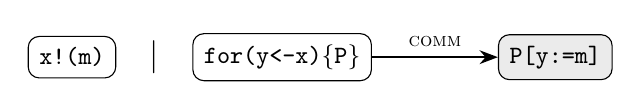
\begin{tikzpicture}[>=Stealth,
  box/.style={draw, rounded corners, align=center, inner sep=4pt,
    font=\small\ttfamily}]
  \node[box] (s) {x!(m)};
  \node (par) [right=3mm of s, font=\large] {$\mid$};
  \node[box] (r) [right=3mm of par] {for(y<-x)\{P\}};
  \node[box, fill=black!8] (out) [right=16mm of r] {P[y:=m]};
  \draw[->, thick] (r) -- node[above, font=\scriptsize\sffamily] {\textsc{comm}} (out);
\end{tikzpicture}
\caption{A reaction: a send and a matching receive on channel \code{x} rendezvous; the
  receiver continues with the message substituted in.}
\label{fig:rho-comm}
\end{figure}

The rest of the vocabulary is small. \code{0} is the inert process; \code{P | Q} runs
\code{P} and \code{Q} concurrently. Two reflection operators connect processes and names:
\code{@P} \emph{quotes} a process into a name, and \code{*x} \emph{drops} (runs) the process
a name quotes, with \code{*@P = P}. Channels are themselves quoted processes --- this is
what makes the calculus higher-order. \CeTTa{} implements exactly these six strict-core
constructors --- \code{rho:nil}, \code{rho:par}, \code{rho:send}, \code{rho:recv},
\code{rho:quote}, \code{rho:drop} --- with \textsc{comm} as the only reduction. A program is
reduced to quiescence by \code{cetta --lang rhocalc \textit{file}}
(Listing~\ref{lst:t10}), written either in a
MeTTa-style S-expression syntax (\code{.mrho}) or a Rholang-like syntax (\code{.rho}); the
runtime keeps a live index of sends and receive-sites, rebuilt after each reaction.  The
deterministic (canonical) scheduler selects the key-least successor by streaming candidate
keys against the best bound found so far instead of materializing and sorting the whole
frontier, which keeps single-step selection cheap on wide parallel terms.

\subsection{Reflection is enough}
\label{sec:rho-reflection}

A surprising amount follows from \textsc{comm} and quote/drop alone, with no further
primitives. Each item below is a standalone \code{-{}-lang rhocalc} program.
\begin{itemize}
\item \emph{Name mobility.} A receive that drops its argument, placed beside a send carrying
  a quoted send, reduces to that inner send made live: a name has travelled across a channel
  and been activated.
\item \emph{Fresh names.} Quoting a distinct process yields a distinct name, so a receiver
  can mint and use a name it never mentioned syntactically.
\item \emph{Replicated input.} An input-guarded server can re-create its own listener:
  after serving a message it leaves a copy of the receiver in the residual, so the channel
  keeps serving. Persistent receive is \emph{derived}, not built in.
\item \emph{Recursion and divergence.} The same self-recreation, left ungated, runs without
  bound (the engine reports its reduction limit); recursion needs no dedicated operator.
\end{itemize}
Private channels and information hiding come along for free: a payload exchanged on a name
no other process holds is unobservable apart from whatever completion signal the protocol
chooses to publish.

The capstone is \emph{eval-at-\textsc{comm}}. Let the receiver do nothing but drop what it
receives:
\[
  \texttt{eval\_drop}(x,p)\;\equiv\;
  \underbrace{x!(@p)}_{\text{send the quoted program } p}\;\big|\;
  \underbrace{\mathsf{for}(y \leftarrow x)\{\,*y\,\}}_{\text{run whatever arrives}}.
\]
The \textsc{comm} delivers the name \code{@p}; the drop \code{*@p} runs \code{p}; the
process settles at the result of running \code{p}. A handshake has become an evaluation
step, and since \code{p} may itself evaluate to more process, a reaction can plant the next
reactions.

\subsection{Profiles}

A \emph{profile} names a variant of the reduction relation together with the grammar it
accepts. \code{strict-core} is the pure asynchronous spine above: it admits only the six core
constructors, and a non-core form is \emph{rejected} rather than left inert. The \code{cost}
profile accepts a richer resource-annotated dialect in which every reaction must be
\emph{funded} from purses located on its channel, and every run emits a causal receipt of
its spending (Section~\ref{sec:rho-cost}).

\subsection{Certified reduction}
\label{sec:rho-lean}

Does eval-at-\textsc{comm} report the result of running the payload, or could the machinery
quietly change the answer? We settle this in Lean. Run \code{eval\_drop(x,p)} to quiescence
and collect every outcome observable \emph{up to structural rearrangement} of the process;
that set is exactly the results a correct evaluation of \code{p} would produce, and the
statement refers only to what is observable, never to an internal ``this is the answer''
tag. The theorem \code{rhometta\_bridge\_scObserved} (in \code{RhometaReduction.lean})
equates the concrete quiescent run of \code{eval\_drop(x,p)} with
\code{RhometaSCObservedOutcomes} of the same process --- the outcomes visible up to
structural congruence --- with no result-certificate carried in the answer. Two ingredients
are load-bearing. First, a complete canonical-form normalizer \code{nfAtom}: two processes
are structurally congruent exactly when their normal forms coincide, which unblocks
inductions that otherwise stall on the symmetry and transitivity of congruence. Second, one
hygiene side condition \code{noBoundUnderQuote}: the communicated variable must not occur
under a quote, since a payload that hides a bound occurrence inside a quoted name defeats the
characterization (a concrete counterexample exhibits exactly that failure). The development
carries no \code{sorry}, and on 27 October the bridge theorem's axioms were exactly
\code{propext}, \code{Classical.choice} and \code{Quot.sound}. A separate caveat on the trusted
base: its conformance and DSL fixtures use \code{native\_decide}; the bridge theorem's own module
does not.

\subsection{rhometta: MeTTa at the reaction}

eval-at-\textsc{comm} becomes a way to program once the payload is a MeTTa term. The library
\code{lib/rhometta.metta} provides \code{rhometta:eval}, which defers a MeTTa term as the
payload to be run at \textsc{comm}; \code{rhometta:run}, which reduces a process to its
quiescent outcome set; and \code{rhometta:transitions}, which returns one-step successors. It
sits on \code{lib/rho.metta}, the strict-core constructor syntax, and delegates all
reduction to the engine. One consequence is central: when a deferred payload evaluates to
\emph{several} results, the \textsc{comm} forks --- one successor per result. Nondeterministic
computation becomes a branching reaction, and \code{rhometta:run} returns one residual per
branch (the \emph{may-set}).

\subsection{What reactions compute}

\paragraph{The minimal cell.} The smallest rhometta program is a single cell: a send carrying
a deferred term beside a receiver that drops (runs) it. \code{rhometta-eval-cell} sends
\code{(+ 2 3)} this way and the reaction leaves \code{5}; with a multi-result payload
\code{(superpose (a b c))} the \textsc{comm} forks into one branch per result, and
\code{rhometta:transitions} confirms the fork is a single reduction step with three
successors. Communication does computation, and result-multiplicity becomes branching.

\paragraph{A self-unfolding prover.} Seed a \emph{single} cell for a goal. Each \textsc{comm}
evaluates one backward-chaining step whose result is the cells for that goal's subgoals, so
\code{rhometta:run} keeps reducing and the reaction network unfolds itself into a proof tree.
Where a goal has several rules the payload has several results, so the \textsc{comm} forks:
\code{rhometta:run} returns one quiescent residual per complete proof tree
(Figure~\ref{fig:rho-tree}) --- two for the sample ``can I bake a cake?'' goal, while a
single-rule goal stays confluent at one.

\begin{figure}[h]\centering
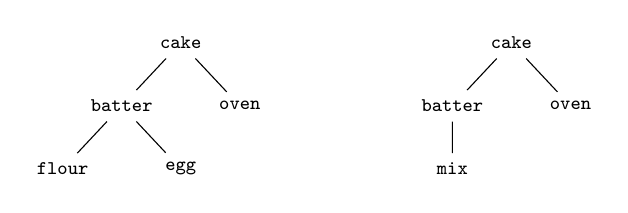
\begin{tikzpicture}[>=Stealth, level distance=8mm, sibling distance=15mm,
  every node/.style={font=\scriptsize\ttfamily}, edge from parent/.style={draw,-}]
  \begin{scope}
  \node {cake} child { node {batter} child { node {flour} } child { node {egg} } }
               child { node {oven} };
  \end{scope}
  \begin{scope}[xshift=42mm]
  \node {cake} child { node {batter} child { node {mix} } }
               child { node {oven} };
  \end{scope}
\end{tikzpicture}
\caption{The self-unfolding prover's may-set for ``cake'': two complete proof trees, one per
  rule for \code{batter}. The trees are not enumerated up front --- they are \emph{grown} by
  reactions whose payloads plant their children.}
\label{fig:rho-tree}
\end{figure}

\paragraph{Type inference as proof search.} A typing judgment \code{(: proof (HasType e t))}
is proved by reactions over typing rules, and the proof term is the derivation. In
\code{rhometta-type-inference}, an overloaded \code{plus} yields a genuine may-set --- an
\code{Int} and a \code{Float} typing of \code{(plus one one)} --- while \code{(plus x one)}
with \code{x : Int} prunes the \code{Float} branch at the unification join. Proof terms stay
pure, \code{(: (app pf pa pb) (HasType e t))} --- a typing is crisp, so no truth value is
attached. Each result is cross-checked differentially against a sequential
chainer over the same knowledge base, which derives the same proof-term skeletons.

\paragraph{A truth value that is earned.} Crisp proof terms are the right output for a typing,
but some judgments are genuinely probabilistic, and there a reaction can carry evidence rather
than certainty. In \code{rhometta-evidence-revision}, two agents each count their own
observations of ``ravens are black'' into an opinion --- a strength and a confidence ---
computed at \textsc{comm} by a deferred payload. The two agents share two observations, so
merging their opinions \emph{naively} double-counts the shared evidence and overstates the
confidence ($0.889$); an overlap-corrected revision discounts the shared stamps for the honest
value ($0.857$), at the same strength. The revision can run after the parallel fan-in, or
\emph{at} the final rendezvous itself. This is the one place a truth value belongs --- it is
counted from data, not attached by hand.

\paragraph{Composition.} These pieces compose: a further program runs an independent proof
search, an overlap-corrected evidence revision, and an attention-spreading step concurrently,
then rendezvouses their channel-gathered results into a single synthesis.

\subsection{Cost-accounted reactions}
\label{sec:rho-cost}

A reaction is the natural unit of metering: each \textsc{comm} is one indivisible piece of
work. The \code{cost} profile makes that intuition operational --- and it does so with money
rather than a stopwatch. Processes are \emph{signed}, channels carry \emph{purses} of
tokens, a reaction fires \emph{only if it is paid for}, and what a run returns is not a
number but a \emph{receipt}: a causal, auditable record of every spend. The profile is the
executable part of the programme to equip the $\rho$-calculus with compositional resource
accounting~\cite{costendofunctor,rhocost-companion}. Its design commitments are locality of
funding, causality from consumption, and an explicit separation between exact authority
receipts and lossy numerical valuations.

\paragraph{Purses and funded reactions.} In the \code{.rho} syntax, \code{\{P\}alice} is
the process \code{P} signed by \code{alice}, and \code{purse pay \{alice : ()\}} is a store
on channel \code{pay} holding one token signed by \code{alice}. The funding rule is
\emph{located}: a \textsc{comm} on \code{pay} consumes one token per participating endpoint
signature, and those tokens must be found in purses \emph{on \code{pay} itself}. There is no
ambient bank account, and raw process data never funds anything. The smallest funded program
has two signed endpoints and two purses
(\href{https://github.com/zariuq/CeTTa/blob/e23de3043462d80e27f9c9009bd0f1b955ed140c/tests/rhocalc_cost_run/split_tokens_basic.rho}{\code{tests/rhocalc\_cost\_run/split\_tokens\_basic.rho}}):

\begin{lstlisting}
{for ($m <- pay) {{0}cont}}alice | {pay!({0}payload)}bob
  | purse pay {alice : ()} | purse pay {bob : ()}
\end{lstlisting}

\noindent
which reduces to \code{purse pay \{()\} | purse pay \{()\} | \{0\}cont} (rerun on 27 October on
the pre-main binary, with this and the next two examples' expected outputs reproduced exactly):
each signature paid
for its own endpoint, and the two purses are left empty beside the continuation. Now delete
\code{bob}'s purse
(\href{https://github.com/zariuq/CeTTa/blob/e23de3043462d80e27f9c9009bd0f1b955ed140c/tests/rhocalc_cost_run/missing_token_quiescent.rho}{\code{missing\_token\_quiescent.rho}}) and
the program is \emph{quiescent with the send and receive still facing each other}: the
reaction is not slowed, it is \emph{disabled}. This is the first thing to internalize about
the profile --- cost is not an observer bolted onto the side; an unfunded reaction cannot
fire. Because channels are quoted processes, a purse's location follows the calculus's own
name equivalence rather than spelling: a purse on \code{@\{*pay\}} funds a reaction on
\code{pay}, since the two names denote the same channel
(\href{https://github.com/zariuq/CeTTa/blob/e23de3043462d80e27f9c9009bd0f1b955ed140c/tests/rhocalc_cost_run/name_equivalence_quote_drop.rho}{\code{name\_equivalence\_quote\_drop.rho}}) ---
aliases of a channel are the same account.

\paragraph{Receipts are causal records, not counters.} A single number would forget who
paid, what was consumed, and what depended on what --- and its intermediate readings would
depend on which interleaving the scheduler happened to choose. Instead, every reaction emits
an event record with four fields: a fresh event identifier; a \emph{cause list} --- the
identifiers of the events that produced the exact occurrences this event consumed, with
repetitions kept (consuming two outputs of event $0$ yields the cause list \code{(0 0)}); a
nonempty list of \emph{funding} records naming the purse location and head signature of each
token spent; and the consumed signature itself. The two-reaction chain below (the first case
of
\href{https://github.com/zariuq/CeTTa/blob/e23de3043462d80e27f9c9009bd0f1b955ed140c/tests/test_lts_rho_cost_causal_trace.metta}{\code{tests/test\_lts\_rho\_cost\_causal\_trace.metta}})
shows the shape --- event $1$ consumes both a continuation and a purse tail produced by
event $0$, so its cause list holds two arcs to $0$:

\begin{lstlisting}
(lts:rho:cost:receipt
  ((lts:rho:cost:event 0 ()
     ((lts:rho:cost:funding chain spend)) spend)
   (lts:rho:cost:event 1 (0 0)
     ((lts:rho:cost:funding chain spend)) spend))
  (rho:cost:par
    (rho:cost:purse chain rho:cost:stack-empty)
    (rho:cost:signed rho:nil done)))
\end{lstlisting}

The algebraic reading is the load-bearing one. A receipt is a \emph{located, measured
pomset} of spend events: a partially ordered multiset whose order is generated purely by
consumption --- event $e'$ follows $e$ exactly when $e'$ consumed something $e$ produced.
The engine's emission order is one linearization of that partial order.  Any
permutation of one fixed compatible matching yields the same target and receipt
bag; the emitted sequence linearizes that matching's causal order.  Alternative
endpoint or funding matchings remain distinct branches.  The Lean theorem
\code{boundedBudgetedCausalPrefix\_emission\_linearizes} confirms that a budgeted
prefix's emitted sequence linearizes its causal order. Locations make purses \emph{fibers} over channels: funding
never crosses a channel, and each per-location account is conserved
(\code{CostPath.per\_location\_restriction\_account\_conservation}). Finally, the receipt
itself carries no notion of ``the cost'': costs are \emph{valuations} --- monoid-valued maps
out of the receipt (total spend, per-signature spend, critical-path depth) --- so the
receipt is the free object and each accounting policy is a homomorphism out of it, with the
lawful combination rules derived rather than posited, in the sense of Knuth and Skilling's
measure-assignment axioms~\cite{knuthskilling}. Event identifiers are deliberately
polymorphic in the same spirit: a local counter suffices in one process, and a hash-chained
identifier can replace it at trust boundaries with the receipt algebra unchanged.

\paragraph{Honest budgets.} Everything above is unbounded by default:
\code{lts:rho:cost:steps} and \code{lts:rho:cost:causal-trace} enumerate exactly and never
truncate silently. Bounded execution is strictly opt-in through
\code{lts:rho:cost:causal-prefix}, which takes two separate allowances --- reaction fuel and
exact-cover search work --- and returns a receipt together with a status that never lies:
\code{quiescent} only after exhaustive search \emph{proves} the residual has no funded
successor; \code{fuel-exhausted} when the firing allowance ends first;
\code{search-exhausted} when cover search stops before finding a successor \emph{or proving
absence}. Search exhaustion is never reported as quiescence: an out-of-fuel machine says ``I
ran out,'' never ``there was nothing there.'' The distinction has teeth because funding
search is a genuine exact-cover problem. A send whose signature product multiplies ten
\code{coin}s, beside twenty unit purses on the same channel, admits
$\binom{20}{10}=184{,}756$ distinct covers
(\href{https://github.com/zariuq/CeTTa/blob/e23de3043462d80e27f9c9009bd0f1b955ed140c/tests/test_lts_rho_cost_search_budget.metta}{\code{tests/test\_lts\_rho\_cost\_search\_budget.metta}}):

\begin{lstlisting}
; Zero reduction fuel performs no exact-cover search, even when
; the latent cover family has C(20,10) members.
!(assertEqualToResult
  (test:prefix-status
    (lts:rho:cost:causal-prefix 0 0 (test:large-cover-state)))
  (lts:rho:cost:fuel-exhausted))

; The first exact occurrence cover is yielded without
; materializing the other 184,755 covers.
\end{lstlisting}

\noindent
At fuel $0$ the machine performs no search at all; with a small search allowance it yields
the first cover lazily; and the unlimited frontier remains available and exact --- all
$184{,}756$ successors, measured at about $11$\,s --- combinatorial by design and by
request, never by accident. A budget-monotonicity gate (59 paired runs at increasing
allowances) checks that raising an allowance never flips a determinate verdict and never
removes a receipt event: more fuel can only extend what is known.

\paragraph{Certified correspondence.} The formal side lives in the \code{Cost/}
theory in the Mettapedia repository: cost steps, paths, receipts, valuations,
conservation laws, and a budgeted executor, proven equal to one another where they meet.
The capstone \code{BudgetedPrefixPathRefinement} states that every budgeted machine run
produces a prefix of the occurrence-bearing Lean executable \code{CostPath}, with
the same receipt and the correct status,
and its corollaries pin each verdict separately: sufficient allowances yield an actual
path; exhaustive candidate failure --- unlike bounded exhaustion --- certifies quiescence;
zero fuel and zero search-work report their own exhaustion and make no negative claim. The
machine frontier is proven sound and complete up to structural equivalence
(\code{costStep\_sound\_runtime},
\code{costStep\_complete\_runtime\_up\_to\_struct}); these are the separate
one-step correspondences with the declarative \code{CostStep} relation.
The compositional theorem
\code{budgetedCausalPrefix\_exists\_rhoLanguageDefRewritePath} closes the
corresponding path square for the Lean executor: every publicly admitted
budgeted run yields an occurrence-bearing runtime path, a declarative funded
trace, and a rewrite path in the pure GSLT mechanically derived from
\code{rhoCalc}, with exactly one pure step per runtime firing.

The pure-rho boundary is theorem-backed as well.  The source rho
\code{LanguageDef} supplies the strict syntax and primitive COMM definition;
its compiled matcher, normalization, substitution, and supported COMM contracta
are proved to agree with the independently established semantic development.
The pure GSLT used for erasure is itself derived from that source declaration;
full equivalence of its complete contextual relation with the independently
established relation remains a named theorem obligation.  On the derived
binder-safe fragment, initialization and funded reduction preserve scope; each
declarative \code{CostStep} erases to one derived pure \textsc{comm}, and each
declarative funded or executable path erases to a derived rho rewrite path whose
length is exactly its ordered demand-receipt length.  The equivalence used here
is pure structural congruence: no executable free-Drop step is admitted.  The
canonical configuration erasure is defined by quotient lifting rather than by
a noncomputable representative choice.  The pure-erasure binder-safety judgment
covers exactly syntax observable by pure erasure.  The separate public
runtime-scope check validates every raw field, including purse locations, and is
proved to imply the erasure-domain judgment.
A rerunnable Lean audit prints the axioms of the exported results; they use only Lean's
standard quotient and classical infrastructure, with no project axiom and no unfinished
proof.

On the compiled side, 146 sequential/threaded prefix cases agree, and 308 compiled-C
receipts replay as Lean derivations while two altered receipts are rejected.  The complete
runtime suite passes in the ordinary, thread-sanitized, and address/undefined-behavior
sanitized builds.  The differential harness
(\href{https://github.com/zariuq/CeTTa/blob/e23de3043462d80e27f9c9009bd0f1b955ed140c/scripts/rhocalc_cost_differential.py}{\code{scripts/rhocalc\_cost\_differential.py}})
drives the same terms through the C engine and the Lean executor, including fuel-$0$ and
fuel-$1$ boundary cases, with an out-of-fragment case correctly rejected. This remains
bounded differential evidence about the compiled engine, not a universal theorem about C.

\paragraph{Parallel funded execution.} Compatible reactions execute in OS threads in
waves.  Before a worker can fire, it atomically claims the exact endpoint occurrences and
the exact funding-cover occurrences in a fixed resource order; a wave admits only pairwise
disjoint claims.  The sequential semantics therefore remains the reference, while the
threaded implementation is tested as a legal parallel refinement: both threaded CLI modes,
six contention and disjointness stress families, and the sequential/threaded prefix gate
exercise same-channel disjoint reactions, competing funding covers, duplicate-looking
occurrences, and causal receipt linearization.  Receipt emission is an \emph{optional
observer} on this path: operational components are plain terms, causal provenance rides in a
parallel producer vector, and a scripted transparency gate checks that a state-only run and a
receipt-observed run consume identical resources and reach the same residual.  These gates,
together with thread and memory sanitizers, are implementation evidence; the Lean step/path
theorem above supplies the declarative semantic boundary.

At the modeled parallel boundary, a list of enabled runtime candidates whose
complete endpoint-and-funding source-index family is globally duplicate-free
lifts to a \code{SelectedRuntimeWave}.  Its witnessed source partition
constructs an exact \code{CostMatching}, and every permutation of that fixed
matching serializes as an ordinary declarative cost trace.  This discharges the
runtime-model wave-to-matching square under the occurrence-claim postcondition;
the compiled-C correspondence remains the bounded differential, receipt-replay,
and sanitizer evidence stated above rather than a universal theorem about C.

\paragraph{A strict source LanguageDef and the corrected algebra.} The profile implements
funded rho and no Datalog architecture.  Its strict syntax and primitive \textsc{comm}
definition come from the source \code{LanguageDef}; the compiled artifacts are
proved to agree with the established pure semantics on supported COMM contracta,
while the GSLT used for the cost-erasure theorem is mechanically derived from
that source declaration.  Other implementations are bounded encoding
references, and their executable free-Drop rule is not part of this profile.

The formalization also identifies why the original ordinary-monad faithfulness claim cannot
be repaired by choosing a more cancellative signature monoid.  Joint injectivity of a monoid
multiplication together with a two-sided unit forces the carrier to be a subsingleton; words,
multisets, and numerical costs all forget some factorization.  The landed repair is an
Atkey-style pre/post-indexed semantics~\cite{atkey}: a funded execution has complete source
and target resource states, so incompatible funding transitions are untypeable.  Exact
authority receipts compose without erasure; price and budget totals are explicit,
generally non-injective observations of those receipts.  This is the resource-transition
specialization of the wider graded and parameterized-effect account
~\cite{katsumata,orchard-wadler-eades}.  The companion theory paper states the obstruction,
the indexed laws, and the authority/observation factorization precisely
~\cite{rhocost-companion}.

\paragraph{The continued category and repeated Cost.}  Since the July
development, the Lean side
(\href{https://github.com/zariuq/MeTTapedia/blob/main/lean/mettapedia/Mettapedia/GSLT/LanguageDef/ContinuedCategory.lean}{\code{GSLT/LanguageDef/ContinuedCategory.lean}},
\href{https://github.com/zariuq/MeTTapedia/blob/main/lean/mettapedia/Mettapedia/GSLT/LanguageDef/Cost/Construction.lean}{\code{Cost/Construction.lean}})
treats Cost not as a one-off wrapping of rho but
as a construction on \emph{continued interactive GSLTs}: a language
mechanically derived from one source \code{LanguageDef}, equipped with
one ordered interaction cut (a contact constructor plus program and
environment operands with selected continuation positions), a computable
canonical section of every typed open fiber, and a
\emph{position-sensitive continuation-retyping plan} under which every
non-principal constructor receives a hereditarily wrapped copy while the
two principals receive cut-aware base copies whose continuation parameter
alone moves to the wrapped fiber.  The generated funded language --- the
base/wrapped signature plus a small contact/signing/funding apparatus and
exactly one whole-redex rewrite that consumes a funding-stack head and
carries the tail through --- is itself such an object, and the
object-closure laws of the resulting endofunctor programme are largely
discharged generically: bare-collection constructors of the generated
language are provably non-principal at the next layer, the generated
interaction envelope is stable under the next retyping, a single
declaration-derived typing morphism validates the next layer's signature,
and the typed transport along a retyping plan is proved over the minimal
non-circular signature (theory, cut, plan).  The remaining generated-object
laws are active work with identified routes.  Two corrections landed on the
way and are recorded as compiled counterexamples rather than folklore: the
global raw fiber-stability hypothesis of the earlier normalization
architecture is \emph{false} for rho (a mixed-colour reflective generator
has a typed left endpoint whose canonical right endpoint is ill-typed), and
its repair carries the entire equational theory on \emph{typed} open
carriers with proof-relevant region-tree elaboration --- raw-to-typed
lifting exists only edge-wise, with both endpoints certified in the same
typed fiber.  Exact typed canonical laws then cut out the full subcategory
of \emph{Cost-canonical} objects, which, ordered by collision-free
structural canonical keys, is the honest domain of strict
$\mathrm{Cost}_1$.  The theory paper develops all of this precisely
~\cite{rhocost-companion}; the engine consequence is concrete: the same
source declaration that generates this profile's grammar and its single
funded rewrite is the object the endofunctor consumes, so iterated
cost-accounting is a construction on the specification, never a second
hand-written engine.  The public API is
\href{https://github.com/zariuq/CeTTa/blob/e23de3043462d80e27f9c9009bd0f1b955ed140c/lib/lts/rho/cost.metta}{\code{lib/lts/rho/cost.metta}};
the engine is
\href{https://github.com/zariuq/CeTTa/blob/e23de3043462d80e27f9c9009bd0f1b955ed140c/src/rhocalc_core.c}{\code{src/rhocalc\_core.c}}.
Runnable showcases ship with the engine in \code{examples/rho/} --- a funded vending machine
(an unfunded order left facing a live endpoint), a causal notary chain whose receipt is the
provenance audit trail, an honest-budget meter exhibiting all three prefix verdicts and a
two-cover spend, and a threaded settlement wave whose residual is byte-identical at every
thread count --- each with expected outputs checked by the test suite, alongside a documented
walkthrough of the calculus, both syntaxes, and the profile.

%% ────────────────────────────────────────────────────────────────────
\section{Cross-Runtime Benchmarks}
\label{sec:benchmark-programs}

The rows in this section were measured between June and September 2026, on
the commits named with them, and are kept as dated receipts; several engines
and lines have changed since.  The October measurements of each line of
development are in Section~\ref{sec:lines}.

Benchmark artifacts are labeled by dialect route.  A row may be
\emph{shared} (one dialect-agnostic source), \emph{\PeTTa{}-native},
\emph{\HE{}/\CeTTa{}-native}, mechanically translated, or hand-normalized
after translation to expose the same algorithmic contract in both
dialects.  \HE{} and \PeTTa{} are different MeTTa dialects, so a real
comparison is not ``whatever file happens to run''; it is a named pair of
artifacts plus a stated output contract.  Timing rows in this section
were measured on 2026-06-27 (the pre-GC tree), except the grounded
genomic-inference rows (PLN evidence core, full WM-PLN raw-loader,
mine$\to$chain focus, and deep genomic backward chaining), which were
re-receipted on 2026-07-02 on commit 9237afd; rows explicitly described
as excluded, methodological, or unresolved carry their own status.  The
two heavy genomic rows (full WM-PLN raw-loader and deep genomic backward
chaining) were re-measured on a quiescent host with the same binary at
commit 9237afd; because the two engines are always compared within one
session, the cross-engine ratios are the load-bearing claims.  For rows
whose single-run wall time is below 0.1\,s, we report averaged
full-process wall time over repeated invocations to avoid timer
quantization.  Output is verified identical across runtimes whenever a
row is presented as a clean cross-runtime benchmark.  So a reader can see
precisely what is measured, each subsection below opens with the core of
the program it runs; the full sources are linked inline and collected at
\href{https://github.com/zariuq/CeTTa/tree/07928677c0237a19b2f3c32dffca28d7d2626723/benchmarks/chaining_crossengine}{\code{benchmarks/chaining\_crossengine}}.

Most of the inference benchmarks are driven by one small dependent-typed
\emph{backward chainer}.  To prove a goal \code{(: \$proof \$theorem)} it
either matches a fact in the knowledge base, or---for a rule application
\code{(\$rule \$prem)}---looks up the rule's type and recurses on its
premise (the binary and $n$-ary cases follow the same shape):
\begin{lstlisting}[language={},basicstyle=\ttfamily\scriptsize]
(: bc (-> $a Nat $b $b))                                  ; KB, depth, goal -> goal
(= (bc $kb $_ (: $proof $theorem))                        ; base case: it's a fact
   (match $kb (: $proof $theorem) (: $proof $theorem)))
(= (bc $kb (S $d) (: ($rule $prem) $theorem))             ; step: apply a rule
   (let* (((: $rule (-> (: $prem $t) $theorem))
            (bc $kb $d (: $rule (-> (: $prem $t) $theorem))))
          ((: $prem $t) (bc $kb $d (: $prem $t))))
     (: ($rule $prem) $theorem)))
\end{lstlisting}
Each benchmark below supplies its own typed rules and facts to this
chainer (or, where noted, a forward chainer or a truth-value kernel).

\subsection{Shallow Evaluation}

Nil Geisweiller's typed backward chainer (the \code{bc} above) over
60 ground entities at depth~1 (20 researchers, 20 engineers, 20
artists).  The rules are typed binary implications; for example,
\code{r-mortal} combines a researcher fact with a curious fact to
derive a mortal witness:
\begin{lstlisting}[language={},basicstyle=\ttfamily\scriptsize]
(: r-mortal (-> (: $r (researcher $x))
                (: $c (curious $x))
                (mortal $x)))
!(bc &kb (fromNumber 1) (: $proof (mortal $x)))      ; -> 60 witnesses
\end{lstlisting}
All three runtimes produce identical 60 proof-carrying witnesses, e.g.\
\code{(: (r-mortal r01 r01c) (mortal r01))}.

\begin{center}
\begin{tabular}{lrrl}
\toprule
Runtime & Time & vs.\ \CeTTa{} & Output \\
\midrule
\CeTTa{} & 4.0\,ms avg  & 1$\times$           & 60 witnesses \\
\PeTTa{} & 45.4\,ms avg & 11.3$\times$ slower & 60 witnesses \\
\HE{}    & 402\,ms avg  & 100$\times$ slower  & 60 witnesses \\
\bottomrule
\end{tabular}
\end{center}

This is a startup-dominated sanity row, not a scaling claim.  It is
useful because it exercises the typed proof-carrying API while
remaining small enough that translator and runtime drift are easy to
spot.

\subsection{Deep Proof Search: \PeTTa{} Wins}

Metamath proof search at depth~5 (2 axioms, proving $t = t$,
85{,}013 proof trees) reverses the performance ordering.  The knowledge
base is Geisweiller's \code{demo0} (axiom \code{a1}: equality is
right-Euclidean; \code{a2}: $0$ is a right identity; \code{mp}: modus
ponens), and the goal is \code{t = t}
(\href{https://github.com/zariuq/CeTTa/blob/07928677c0237a19b2f3c32dffca28d7d2626723/benchmarks/chaining_crossengine/01_nilbc/nilbc_th1.metta}{\code{01\_nilbc/nilbc\_th1.metta}};
glyphs shown ASCII here):
\begin{lstlisting}[language={},basicstyle=\ttfamily\scriptsize]
(: a1 (-> (: $t term) (: $r term) (: $s term)
          (-> (= $t $r) (-> (= $t $s) (= $r $s)))))   ; right-Euclidean
(: a2 (-> (: $t term) (= (+ $t 0) $t)))               ; 0 right-identity
(: mp (-> (: $maj (-> $P $Q)) (: $P wff) (: $Q wff)
          (: $min $P) $Q))                            ; modus ponens
!(bc &kbh (fromNumber 5) (: $prf (= t t)))            ; prove t = t
\end{lstlisting}

\begin{center}
\begin{tabular}{lrrl}
\toprule
Runtime & Time & vs.\ \PeTTa{} & Status \\
\midrule
\PeTTa{} & 7.60\,s  & 1$\times$          & 85{,}013 proofs \\
\CeTTa{} & 36.42\,s & 4.8$\times$ slower & 85{,}013 proofs \\
\HE{}    & $>$120\,s & timeout            & killed \\
\bottomrule
\end{tabular}
\end{center}

\PeTTa{}'s Prolog search remains decisively better on deep branching
proof search; the current rerun widens the gap to roughly
4.8$\times$.  \HE{} still cannot finish within 120\,s.

\subsection{Forward Chaining at Scale}

Nil Geisweiller's propositional-calculus forward chainer at depth~4
uses a solution space that is extended in place by forward application
of modus ponens:
\begin{lstlisting}[language={},basicstyle=\ttfamily\scriptsize]
(= (fs-add-to-ss $rb $ss)
   (with-space-snapshot $ss0 $ss
     (match $ss0 (: $x1 $a1)
       (match $ss0 (: $x2 $a2)
         (match $rb (: $f (-> $a1 $a2 $b))
           (add-atom $ss (: ($f $x1 $x2) $b)))))))
!(count-atoms &ss)
\end{lstlisting}
The current \CeTTa{} rerun of
\href{https://github.com/zariuq/CeTTa/blob/07928677c0237a19b2f3c32dffca28d7d2626723/tests/nil_pc_fc_d4.metta}{\code{tests/nil\_pc\_fc\_d4.metta}}
completes in 100.86\,s and reports 8.19M accumulated results after the
four forward passes.  We do \emph{not} reuse the older
``11.7M generated pairs'' sentence as benchmark evidence, because the
current HE lane does not time out on this driver; it errors immediately
(\code{match expects a space as the first argument}).  So the forward
row remains a useful workload, but it is not yet paper-ready as a clean
cross-runtime benchmark.

\subsection{Translator Validation}

A PeTTa-native benchmark using \code{prog1} (PeTTa-specific construct)
was translated PeTTa$\to$HE and run on \CeTTa{}.  The translator
converts \code{prog1} to nested \code{let} with fresh variables:
\begin{lstlisting}[language={},basicstyle=\ttfamily\scriptsize]
; PeTTa original:
(= (run-query) (prog1 (bc &kb ...) (println! "done")))
; Translated to HE:
(= (run-query) (let $__tr_result_1 (bc &kb ...)
                 (let $__tr_discard_2 (println! "done")
                   $__tr_result_1)))
\end{lstlisting}
The current source file
\href{https://github.com/zariuq/CeTTa/blob/07928677c0237a19b2f3c32dffca28d7d2626723/benchmarks/bench_backchain_petta_native.metta}{\code{benchmarks/bench\_backchain\_petta\_native.metta}}
produces 30 proof-carrying witnesses on native \PeTTa{}, and the
current translated artifact produces the same 30 witnesses on both
\CeTTa{} and \HE{}:
\begin{center}
\begin{tabular}{lrrl}
\toprule
Runtime & Time & vs.\ \CeTTa{} & Output \\
\midrule
\CeTTa{} & 3.7\,ms avg  & 1$\times$          & 30 proofs \\
\PeTTa{} & 44.8\,ms avg & 12.1$\times$ slower & 30 proofs \\
\HE{}    & 319\,ms avg  & 86$\times$ slower  & 30 proofs \\
\bottomrule
\end{tabular}
\end{center}
This row is a translator benchmark, not just a syntax example: the
observable runtime behavior survives translation.

\subsection{PLN Evidence Aggregation over Genomic KB}

To benchmark inference over real data, we run PLN evidence aggregation
over the Rejuve genomic knowledge base (chr16 pilot: 41~GWAS SNPs,
183~SNP--gene pairs, 3~evidence channels).  Each pair carries
eQTL tissue counts (GTEx, 49~tissues), ABC enhancer--gene contact
counts, and a regulatory presence flag.  The PLN evidence quantale
combines channels via revision (\code{evidence-hplus}), producing a
calibrated SimpleTruthValue per pair.  The evidence operations are
Lean-verified: \code{power}, \code{toLogOdds\_power\_mul}, and
\code{power\_power\_inv} are proved in
\code{Mettapedia/PLN/Evidence/BinaryEvidence.lean}.

The core arithmetic is ordinary MeTTa over numbers:
\begin{lstlisting}[language={},basicstyle=\ttfamily\scriptsize]
(= (Truth_ModusPonens (stv $f1 $c1) (stv $f2 $c2))
   (stv (+ (* $f1 $f2) (* 0.02 (- 1 $f1))) (* $c1 $c2)))
(= (Truth_Revision (stv $f1 $c1) (stv $f2 $c2))
   (let* (($w1 (Truth_c2w $c1)) ($w2 (Truth_c2w $c2)) ($w (+ $w1 $w2))
          ($f (/ (+ (* $w1 $f1) (* $w2 $f2)) $w)) ($c (Truth_w2c $w)))
     (stv (min 1.0 $f) (min 1.0 $c))))
\end{lstlisting}
The benchmark is dialect-agnostic (shared MeTTa, no translation
needed).  The portable
\href{https://github.com/zariuq/CeTTa/tree/07928677c0237a19b2f3c32dffca28d7d2626723/benchmarks/bio_pln}{\code{benchmarks/bio\_pln}}
evidence-score drivers produce numerically identical
183 scored pairs on \CeTTa{}, \PeTTa{}, and \HE{}:

\begin{center}
\begin{tabular}{lrrrl}
\toprule
Runtime & Time & vs.\ \CeTTa{} & Output & Status \\
\midrule
\CeTTa{} & 10.9\,ms avg & 1$\times$ & 183 bio-scores & identical \\
\PeTTa{} & 58.1\,ms avg  & 5.4$\times$ slower & 183 bio-scores & identical \\
\HE{}    & 7.56\,s     & 696$\times$ slower & 183 bio-scores & identical \\
\bottomrule
\end{tabular}
\end{center}

Scores carry genuine biological signal:
\code{rs9923732}$\to$\code{ENSG00000166455} scores strength
0.7348066298342542 ($133/181$) and confidence 0.9945054945054945
($181/182$), while most pairs score 0.04 (minimal evidence).  All three
engines reproduce every one of the 183 scores to full numeric
precision on the portable drivers; the earlier non-portable driver
diverged only because upstream \HE{} integer-divided the evidence ratio
to zero and \PeTTa{} left imported evidence-library calls unreduced.
Exact three-engine numeric agreement is this row's validation story.

\paragraph{What we no longer claim here.}
Earlier drafts included a synthetic scaling table from 143 to
1.4M atoms.  We still do not treat that older synthetic table itself as
benchmark evidence in the paper.  What \emph{is} now grounded again is
the true full raw-loader checkpoint lane: the fresh \CeTTa{} and
\PeTTa{} reruns both execute the same TFBS-inclusive
1{,}399{,}997-line data tier and agree on the labeled observable
contract
(\code{9} seed targets, \code{9} contextual targets, \code{85}
disease proofs, \code{34} supported-drug proof witnesses, and
\code{8} unique supported-drug hypotheses).  The explicit proof-count
vs.\ hypothesis-count split matters here: the \code{34} traces are
genuinely multiple proof routes collapsing to \code{8} unique
\code{(gene,disease,drug,tissue)} hypotheses, not a stale counting
mistake.  Fresh timings on this grounded full row are 16.4\,s on
\CeTTa{} and 44.5\,s on \PeTTa{} (about 2.7$\times$ faster).  Upstream \HE{} does not currently
run this loader shape directly: its \code{metta} runner rejects the
relative-file \code{import! ./support/...} syntax as an illegal module
name, so the \HE{} column for this row remains a loader blocker rather
than a performance number.  The 183-pair core therefore remains the
grounded small PLN row, while the full TFBS-inclusive checkpoint is now
the grounded large WM-PLN row.

\subsection{Genomic Pattern Mining}

To exercise real algorithmic depth, we run the Hyperon pattern
miner~\cite{metta} on real GTEx eQTL data, discovering surprising
co-regulation patterns---pairs of SNPs or genes that share eQTL
evidence more often than expected by independence.  The miner is run
unmodified from
\href{https://github.com/iCog-Labs-Dev/hyperon-miner}{github.com/iCog-Labs-Dev/hyperon-miner};
its core loop alternates \code{build-specialization} (extend a candidate
pattern by one link) with a \code{surprisingness} score that keeps only
patterns whose support exceeds the independence expectation.  The data
is extracted from the Rejuve genomic KB (338M Prolog lines, 57\,GB) and
discretized into categorical attributes (tissue breadth, effect size)
for pattern mining.

The current audit does \emph{not} reuse the older cross-engine mining
speed table as benchmark evidence, and no current in-tree driver
re-emits the earlier specialization-core atom count, so we do not carry
that number forward.  We keep the pattern miner as a methodological
workload because it contains stateful \code{superpose}: a remove/add
pattern that mutates a shared space in the middle of a non-deterministic
branch family:
\begin{lstlisting}[language={},basicstyle=\ttfamily\scriptsize]
(superpose ((remove-atom $specspace $spec1)
            (add-atom    $specspace $spec1)
            (remove-atom $specspace $spec2)
            (add-atom    $specspace $spec2)
            (remove-atom $specspace $spec3)
            (add-atom    $specspace $spec3)))
\end{lstlisting}
The earlier paper classified one observed traversal as correct and another
as atom loss.  Without a current driver and an explicit effect-order
contract, that conclusion is not retained.  The case instead motivates the
factorization in Section~\ref{sec:nondet-state}: compare complete result bags
and multiplicity where the observer is a bag, record effect traces where
effects are observable, and require an explicit mutex, transaction, snapshot,
or sequence policy when the program needs a stronger order.  The miner
therefore remains a portability and stress workload, not a fresh cross-engine
speed or scheduler-correctness table.

\subsection{Backward Chaining over Mined Patterns}

The mined co-regulation patterns serve as typed inference rules for
Geisweiller's \code{nilbc} backward chainer (the same dependent-typed
\code{bc} listed at the start of Section~\ref{sec:benchmark-programs}), closing the
\emph{mine$\to$chain} pipeline.  The knowledge base combines:
\begin{itemize}
\item 100{,}000 real GTEx eQTL links (40{,}484~SNPs $\times$ 14{,}043~genes),
\item 13 co-regulation patterns and 7 co-expression patterns (mined,
  surprisingness $>$\,0.98),
\item 3 typed PLN rules: \emph{direct-target} (eQTL $\to$ target),
  \emph{coreg-transfer} (co-regulation $+$ target $\to$ target), and
  \emph{coexpr-transfer} (target $+$ co-expression $\to$ target).
\end{itemize}
The three rules are typed implications fed to the \code{bc} chainer of
Section~\ref{sec:benchmark-programs}; \emph{direct-target} reads an eQTL
fact, \emph{coreg-transfer} chains a co-regulation edge onto an existing
target:
\begin{lstlisting}[language={},basicstyle=\ttfamily\scriptsize]
(rule-sig dt (-> (: $e (eqtl $snp $gene))            ; direct-target
                 (target $snp $gene)))
(rule-sig ct (-> (: $e1 (coreg $snp1 $snp2))         ; coreg-transfer
                 (: $e2 (target $snp2 $gene))
                 (target $snp1 $gene)))
!(bc &kb (fromNumber 2) (: $proof (target rs10000544 $gene)))
\end{lstlisting}
Bridge base cases let \code{nilbc} consume untyped data atoms
(\code{eqtl-link}, \code{co-regulate}) directly, avoiding a format
conversion pass over the 100K-atom KB\@.

On the portable
\href{https://github.com/zariuq/CeTTa/tree/07928677c0237a19b2f3c32dffca28d7d2626723/benchmarks/mine_chain_focus}{\code{benchmarks/mine\_chain\_focus}}
focus-summary drivers,
\CeTTa{} and \PeTTa{} agree exactly on the distinct direct and depth-2
target genes for three representative query SNPs (the raw proof rows
dedupe by target gene to these counts):

\begin{center}
\begin{tabular}{lrrr}
\toprule
Query SNP & direct targets & depth-2 targets & novel \\
\midrule
rs10000544 & 9 & 12 & 3 \\
rs10000620 & 5 & 5  & 0 \\
rs10000960 & 6 & 8  & 2 \\
\bottomrule
\end{tabular}
\end{center}

The five novel depth-2 targets are:

\begin{center}
\begin{tabular}{llll}
\toprule
Gene & Symbol & Via SNP & Evidence path \\
\midrule
ENSG00000150961 & SEC24D  & rs10000795 & \code{(ct cr3 (dt eq37))} \\
ENSG00000172399 & MYOZ2   & rs10000795 & \code{(ct cr3 (dt eq39))} \\
ENSG00000178636 & MRPL42P1 & rs10000726 & \code{(ct cr1 (dt eq30))} \\
ENSG00000248394 & FOSL1P1  & rs10001048 & \code{(ct cr25 (dt eq87))} \\
ENSG00000273077 & (lncRNA)  & rs10001048 & \code{(ct cr25 (dt eq89))} \\
\bottomrule
\end{tabular}
\end{center}

The proof terms are machine-checkable evidence chains: \code{(ct cr3
(dt eq37))} reads ``co-regulation transfer via \code{cr3}
(rs10000544$\leftrightarrow$rs10000795), applied to direct eQTL
\code{eq37} (rs10000795$\to$SEC24D).''  On these focused three-query
drivers the total wall-clock time is 0.13\,s on \CeTTa{} versus
4.27\,s on \PeTTa{}.  We therefore keep the novel-gene discovery story,
but we do \emph{not} reuse the older proof-count/time row as benchmark
evidence in this paper.

Biologically, the novel discoveries include MYOZ2 (hypertrophic
cardiomyopathy gene, OMIM CMH16) and SEC24D (Cole-Carpenter bone
syndrome), both on chr4q26---suggesting a trans-regulatory link from a
metabolic locus (PDE5A/FABP2) to cardiac and skeletal gene targets via
shared cis-regulatory architecture.

The older ``all 7~query SNPs plus reverse queries'' timing line is not
used as a fresh paper benchmark here; the audited evidence in this
revision is the focused cross-runtime driver above.

\paragraph{Complete benchmark ladder.}
The following table summarizes all benchmarks, including both genomic
inference (where \CeTTa{} wins) and pure search (where \PeTTa{} wins):

\begin{center}
\resizebox{\textwidth}{!}{%
\begin{tabular}{lrrrl}
\toprule
Benchmark & Scale / note & \CeTTa{} & \PeTTa{} & \HE{} \\
\midrule
Shallow typed BC & 60 proof witnesses & 4.0\,ms avg & 45.4\,ms avg & 402\,ms avg \\
Translator (\code{prog1}) & 30 proof witnesses & 3.7\,ms avg & 44.8\,ms avg & 319\,ms avg \\
PLN evidence core & 183 scored pairs & 10.9\,ms avg & 58.1\,ms avg & 7.56\,s \\
Full WM-PLN raw-loader & 1{,}399{,}997 lines, 34 proofs / 8 hyps & 16.4\,s & 44.5\,s & import block \\
Mine$\to$chain focus & 3 query SNPs, 5 novel genes & 0.13\,s & 4.27\,s & --- \\
Deep 17-phase genomic BC & 1{,}411{,}430 hypotheses & 46.33\,s & 64.05\,s & --- \\
8-Queens (direct shared lane) & 92 solutions & 8.22\,s & 0.05\,s & 2:08.77 \\
Deep proof search & 85{,}013 proofs & 36.42\,s & 7.60\,s & $>$120\,s \\
\bottomrule
\end{tabular}}
\end{center}

\noindent\emph{Peak resident memory on the two heavy rows.}  On the full
WM-PLN raw-loader, \CeTTa{} uses 2.10\,GiB against \PeTTa{}'s 4.75\,GiB
(\CeTTa{} lower).  On the deep 17-phase genomic BC the direction
reverses: \CeTTa{} uses 14.5\,GiB against \PeTTa{}'s 4.85\,GiB---about
3.0$\times$ \PeTTa{}'s footprint, the memory-multiplicity cost of
\CeTTa{}'s answer materialization on the high-fan-out row.

\CeTTa{} still wins on several real inference rows, but the revised
ladder is intentionally smaller than earlier drafts.  In the 2026-06-27
audit we excluded the
historical cross-engine miner speed table, the old full-1.4M WM-PLN
scaling table, and BTree from this cross-engine ladder because at that
point the tree either lacked a stable current cross-runtime driver for
them or exposed a correctness/comparability issue.  The tilepuzzle row
has since been rerun and is reported separately as a search benchmark
and GC capacity result in Section~\ref{sec:tilepuzzle-gc}.  The
benchmark rows shown here are only those rerun directly in that audit.

\subsection{Cross-Engine Chaining Suite}
\label{sec:chaining-suite}

To ground the inference-side comparison on community-written code
rather than bespoke benchmarks, we assembled a cross-engine chaining
suite that builds matched cross-engine rows from the same chainer
families on \CeTTa{} (\code{-{}-lang he}) and \PeTTa{}, with a per-row
cross-engine contract (every result is
validated against the other engine's output, never against \CeTTa{}'s
own output).  The sources are
Geisweiller's dependent-typed DTL chainers and Metamath \code{demo0}
proofs (\href{https://github.com/ngeiswei/chaining}{github.com/ngeiswei/chaining}),
Treutlein's \code{PeTTaChainer}
(\href{https://github.com/rTreutlein/PeTTaChainer}{github.com/rTreutlein/PeTTaChainer}),
and the \PeTTa{} engine and its PLN library
(\href{https://github.com/patham9/PeTTa}{github.com/patham9/PeTTa}).
The suite, generators, and driver are in the \CeTTa{} repository under
\href{https://github.com/zariuq/CeTTa/tree/07928677c0237a19b2f3c32dffca28d7d2626723/benchmarks/chaining_crossengine}{\code{benchmarks/chaining\_crossengine}}.
In this paper revision we use the suite as audited reproducibility
material rather than as an extra source of unevaluated claims: the
benchmark rows retained in the paper are only the subset rerun directly
in this audit.

\paragraph{Multi-relational deep chaining.}
The strongest current multi-relational row is the 17-phase snapshot
\href{https://github.com/zariuq/CeTTa/blob/07928677c0237a19b2f3c32dffca28d7d2626723/tests/bench_bio_bc_deep_snapshot_20260327.metta}{\code{tests/bench\_bio\_bc\_deep\_snapshot\_20260327.metta}}.
It extends the mined-pattern chainer with pathway membership,
same-pathway transfer, disease associations, compound--disease
treatment links, and compound--gene binding links.  The full
variant-to-drug row is still a typed backward-chaining program:
\begin{lstlisting}[language={},basicstyle=\ttfamily\scriptsize]
(rule-sig dg (-> (: $e1 (target $snp $gene))
                 (: $e2 (has-disease $gene $disease))
                 (disease-reach $snp $disease $gene)))
(rule-sig td (-> (: $e1 (disease-reach $snp $disease $gene))
                 (: $e2 (treats $compound $disease))
                 (drug-hypothesis $snp $compound $disease $gene)))
\end{lstlisting}
The current rerun produces exactly \textbf{1{,}411{,}430 hypotheses}
across 17 query phases, identical on both runtimes, with the bucket
breakdown:

\begin{center}
\begin{tabular}{lr}
\toprule
Hypothesis bucket & Count \\
\midrule
\code{pw-target} & 613{,}978 \\
\code{deep-pw} & 796{,}964 \\
binding & 11 \\
disease & 11 \\
drug & 210 \\
deep-drug & 240 \\
pathway-reach & 16 \\
\midrule
Total (17 phases) & 1{,}411{,}430 \\
\bottomrule
\end{tabular}
\end{center}

\begin{center}
\begin{tabular}{lrrrl}
\toprule
Runtime & Wall time & Peak RSS & vs.\ \PeTTa{} & Output contract \\
\midrule
\CeTTa{} & 46.33\,s & 14.5\,GiB & 1.38$\times$ faster & 1{,}411{,}430 hypotheses \\
\PeTTa{} & 64.05\,s & 4.85\,GiB & 1$\times$ & 1{,}411{,}430 hypotheses \\
\bottomrule
\end{tabular}
\end{center}

\noindent The current timings still favor \CeTTa{}, but the table makes
the memory tradeoff explicit: this high-fan-out row is one where
\CeTTa{} materializes many answers and pays roughly 3$\times$ \PeTTa{}'s
peak footprint.
The textbook chain
rs10000544 $\to$ PDE5A $\to$ hypertension $\leftarrow$ Sildenafil
composes three independent data sources (GTEx, Hetionet, DrugBank) by
typed backward chaining with proof terms at every step.

\paragraph{Dependent binder encoding.}
PLN rule declarations use \code{(rule-sig name type)} instead of
\code{(: name type)} to avoid a current HE spec limitation: the
\code{(: \$e T)} syntax in arrow-domain positions is treated as a
literal expected type, not a dependent binder, causing \code{BadArgType}
on both HE and \CeTTa{} (see Section~\ref{sec:heprime}).
The \code{rule-sig} encoding is semantically equivalent on all runtimes.

%% ────────────────────────────────────────────────────────────────────
\subsection{Four-Engine Study: JeTTa and MeTTaScript Join the Ladder}
\label{sec:fourengine}

A 2026-07 study extended the ladder with JeTTa (a Kotlin/JVM
ahead-of-time compiler for MeTTa) and, via its upstream slide deck,
MeTTaScript (TypeScript)~\cite{jetta-slides,jetta-review}.  Every timed
run was gated on answer correctness; a fast wrong answer counts as a
failure.  Three findings matter for \CeTTa{}'s roadmap:

\begin{itemize}
\item \textbf{Competence zones, not a single ranking.}  JeTTa dominates
  deterministic arithmetic recursion (its compiler auto-memoizes pure
  recursion: naive Fibonacci runs in $O(N)$); \PeTTa{} dominates
  unindexed nondeterministic search (8-Queens roughly $150\times$ over
  \CeTTa{}) and is the only engine with production tabling and bignums;
  \CeTTa{} keeps near-zero startup and wins indexed knowledge-base
  queries (the mined-chain workload roughly $26\times$ over \PeTTa{});
  on the heaviest typed proof search in the study (the 85{,}013-proof
  Metamath depth-5 run) \PeTTa{} completes in 13.0\,s under its shipped
  8\,GiB stack configuration versus 62.7\,s for \CeTTa{} --- the
  $4.8\times$ margin matching the earlier audited row.  An initial
  rerun under SWI-Prolog's 1\,GiB \emph{default} stack overflowed and
  was briefly misrecorded as an engine failure; the harness, not the
  engine, was at fault.
\item \textbf{The per-call and sharing taxes, measured.}  On naive
  Fibonacci the per-call interpretation costs were approximately
  $0.23\,\mu$s (\PeTTa{}, WAM) versus $9.6\,\mu$s (\CeTTa{} tree walk)
  --- a $\approx 42\times$ machine tax --- while the tabling three-way
  showed declared tabling and auto-memoization both answering
  \code{fib 46} in $0.10$\,s where the untabled tree walk extrapolates
  to tens of hours.  These are the evidence rows behind the abstract
  machine hypothesis (Appendix on MAM) and the call-keyed sharing
  direction in Prime.
\item \textbf{Methodological hazards.}  Auto-memoization silently turns
  repetition-scaled benchmarks into cache-lookup measurements; one
  engine returned fast \emph{wrong} sums through silent 32-bit
  wraparound; and a harness that launches an engine without its shipped
  resource configuration (here, SWI-Prolog's 1\,GiB default stack in
  place of \PeTTa{}'s configured 8\,GiB) manufactures failures that
  read as engine limits.  All three hazards argue for correctness-gated,
  semantics-aware benchmarking rather than wall-clock tables.
\end{itemize}

\subsection{Pinned Candidate Revalidation}
\label{sec:pinned-candidate-revalidation}

The four-engine conclusions above were rechecked on ordinary optimized
binaries against a fixed \CeTTa{} candidate
(\code{7707cef}), JeTTa \code{c95d87d} (version 0.7.0), and the
corresponding pinned \PeTTa{}, HE, and MeTTa-on-MORK revisions.  Timed
cells were admitted only after exact answers agreed; reported values are
medians of five interleaved runs where the harness supports repetition.
Sanitizer runs, failed cells, and semantically unequal cells are not
timing evidence.

\paragraph{Shared-program conformance.}
Twenty of twenty-one selected HE programs produced identical output
bags on HE with GroundingSpace, HE with MORK, \CeTTa{} native space, and
\CeTTa{} explicit \PathMap{} space.  The remaining documentation example
failed on both HE stores and was excluded rather than attributed to a
\CeTTa{} backend.  A separate duplicate-atom discriminator exposed the
important carrier boundary: HE's MORK store collapsed three insertions
to set support, whereas both \CeTTa{} spaces preserved the two requested
occurrences in the query result.  Thus \PathMap{} agreement is not merely
cardinality agreement: \CeTTa{}'s counted encoding preserves the language's
bag contract.

At the pinned \code{7707cef} candidate, the command-line
\code{-{}-space-engine pathmap} route stored only the bootstrap portion in
\PathMap{} and then fell back to the ordinary evaluator space.  The tables
in this historical subsection therefore used explicit
\code{(new-space pathmap)} objects.  This limitation no longer held on
the later 1.4 development line: \code{-{}-space-engine pathmap} made a
counted \PathMap{} inside the Rust bridge's MORK \code{Space} container the
primary occurrence store for generic MeTTa queries.  It uses MORK expression
bytes as trie keys but does \emph{not} run those queries through MM2's
\code{space\_step}; raw MM2 stepping and generic counted queries are distinct
modes over related substrate.

\paragraph{One-million-fact space lifecycle.}
The Roman/friend matrix performs one million insertions, one exact hit,
one exact miss, a full scan, one removal, a post-removal miss, and a
post-removal count.  Every lane returned the same rows and multiplicities.
Table~\ref{tab:roman-friend-refresh} reports whole-process wall time and
peak RSS; the embedded operation timer is shown separately for the exact
hit because it isolates lookup and reconstruction from process startup.

\begin{table}[htbp]
\centering
\begin{tabular}{lrrr}
\toprule
Lane & Wall time & Peak RSS & Exact hit \\
\midrule
\PeTTa{} ordinary space & 0.85\,s & 295\,MiB & 129\,ms \\
\CeTTa{} native space & 4.56\,s & 643\,MiB & 25.2\,$\mu$s \\
\CeTTa{} native $\rightarrow$ resident MORK & 6.53\,s & 1{,}317\,MiB & 113\,$\mu$s \\
\CeTTa{} explicit \PathMap{} & 6.43\,s & 1{,}015\,MiB & 56.3\,ms \\
\CeTTa{} \PathMap{} $\rightarrow$ resident MORK & 4.45\,s & 422\,MiB & 116\,$\mu$s \\
\CeTTa{} resident MORK & 4.46\,s & 349\,MiB & 167\,$\mu$s \\
\PeTTa{} MORK bridge & 13.31\,s & 668\,MiB & 111\,$\mu$s \\
\bottomrule
\end{tabular}
\caption{Pinned Roman/friend lifecycle at one million facts.
Conversion lanes include transfer cost; resident lanes do not transfer the
store for each query.}
\label{tab:roman-friend-refresh}
\end{table}

The table does not support ``always outsource to MORK.''  \PeTTa{}'s
ordinary indexed space wins the complete lifecycle, while resident MORK
offers \CeTTa{} the smallest footprint among its million-fact lanes.
At that candidate, \CeTTa{}'s explicit \PathMap{} exact-hit cost was
dominated by its single-pattern adapter and result reconstruction, not by
trie lookup.
Conversely, transferring a native store before a query loses both time and
memory.  The engineering implication is local: retain resident indexed
stores, push conjunction and folds into their query algebra, and stream or
factorize results instead of repeatedly materializing space tuples.

\paragraph{Conjunctive matching.}
On a generated two-hop join with 400{,}000 edges and 399{,}999 answers,
\CeTTa{}'s stock evaluator took 953\,ms per query and its streamed
conjunctive fast path 797\,ms.  MeTTa-on-MORK's product-zipper query took
819\,ms at the same scale.  These close values have different internal
profiles: MeTTa-on-MORK prunes a multi-pattern product during trie descent,
while \CeTTa{} still reconstructs candidate bindings around a shared
evaluator.  At smaller explicit-store sizes on that candidate, native
\CeTTa{} was faster than its then-current \PathMap{} adapter (31.3\,ms
versus 73.6\,ms at 20{,}000 edges).  The appropriate adoption path is to expose
multi-pattern cursor traversal and bounded row batches through \CeTTa{}'s
backend interface, not to copy data across an FFI boundary for every join.

\paragraph{MAM workload revalidation.}
Table~\ref{tab:mam-refresh} uses the same five semantic workloads across
the engines.  JeTTa's core time excludes JVM startup; its wall/RSS cell
includes it.  \PeTTa{} uses native tail-recursive drivers for the
million-step interpreter and differentiation loops.  A dash means the
exact workload did not complete successfully and is not a performance
number.

\begin{table}[htbp]
\centering
\resizebox{\textwidth}{!}{%
\begin{tabular}{lrrrr}
\toprule
Workload & JeTTa wall/RSS & \PeTTa{} wall/RSS
         & \CeTTa{} HE wall/RSS & \CeTTa{} Prime wall/RSS \\
\midrule
Fibonacci(30)
  & 0.26\,s / 76\,MiB & 0.40\,s / 19\,MiB
  & 15.85\,s / 294\,MiB & 97.09\,s / 11.4\,GiB \\
Interpreter ($10^6$)
  & 1.70\,s / 875\,MiB & 0.80\,s / 19\,MiB
  & --- (allocation failure) & --- (timeout) \\
Differentiation ($10^6$)
  & 2.74\,s / 741\,MiB & 1.40\,s / 19\,MiB
  & --- (allocation failure) & --- (timeout) \\
Synthesis(40)
  & 0.45\,s / 104\,MiB & 0.10\,s / 19\,MiB
  & 0.14\,s / 68\,MiB & 0.66\,s / 139\,MiB \\
Backward chaining(1000)
  & 0.41\,s / 102\,MiB & 0.10\,s / 23\,MiB
  & 0.05\,s / 29\,MiB & --- (stack failure) \\
\bottomrule
\end{tabular}
}
\caption{Pinned MAM-workload revalidation.  Every numeric cell
returned the stated exact checksum before timing.}
\label{tab:mam-refresh}
\end{table}

The refreshed evidence sharpens rather than overturns the competence-zone
picture.  JeTTa's compiled and memoized path is strongest on Fibonacci;
\PeTTa{}'s WAM is strongest end-to-end on the million-step deterministic
loops; and \CeTTa{} HE remains strongest on the low-output deduction row.
Prime's failures and high Fibonacci cost are not presented as a competitive
result: they are the measured obligations for the experimental Need-machine
work---linear administrative cost within a demand path, followed by sound
sharing across repeated pure calls.  Measured again on 27 October, naive
\code{fib 30} takes 0.04\,s on the pre-main \HE{} lane, whose prepared pure
route compiles it, about 0.06\,s on its \PeTTa{} lane, and about 2.6\,s with 271\,MB on
the Prime draft (single runs, Appendix~\ref{app:runs}).

\subsection{August 9 Answer-First Backend and Dialect Audit}
\label{sec:august-backend-audit}

The 1.4 development line was audited again after the revision-pinned
machine and \PathMap{} work.  Every timed row below was admitted only after
the exact answer bag, multiplicity, and boundary answers were checked.
Values are single whole-process observations on the audit workstation, not
publication-quality medians; they are retained as structural regression
evidence and are intentionally kept separate from the five-run tables above.

\paragraph{Counted \PathMap{} conjunction.}
The HexLife witness joins two \code{alive} relations around one
\code{neighbors} relation over triangular boards.
All four configurations return the same normalized pair bag at each scale.

\begin{table}[htbp]
\centering
\begin{tabular}{rrlrr}
\toprule
Cells & Result pairs & Lane & Native & \PathMap{} \\
\midrule
1{,}891 & 10{,}980 & Prime & 0.36\,s / 138{,}512\,kB & 0.34\,s / 135{,}316\,kB \\
1{,}891 & 10{,}980 & \PeTTa{} & 1.84\,s / 328{,}688\,kB & 1.84\,s / 331{,}264\,kB \\
7{,}381 & 43{,}560 & Prime & 2.89\,s / 876{,}992\,kB & 2.53\,s / 851{,}424\,kB \\
7{,}381 & 43{,}560 & \PeTTa{} & 22.21\,s / 2{,}447{,}440\,kB & 22.71\,s / 2{,}452{,}192\,kB \\
\bottomrule
\end{tabular}
\caption{Answer-checked HexLife conjunction on current native and counted
\PathMap{} spaces.  Each cell is wall time / peak RSS for one process.}
\label{tab:hexlife-pathmap-current}
\end{table}

Earlier in the audit the \PathMap{} route exposed an effectively complete
candidate scan.  The repair gives the counted trie one synchronized native
discrimination view for candidate coordinates, while the counted \PathMap{}
remains the occurrence authority.  This is why the current table measures a
real index rather than storage followed by a full native unifier scan.
\PathMap{} crosses over slightly on Prime and reaches \PeTTa{} parity on this
trie-suitable join; the large remaining \PeTTa{} time at the higher scale is
therefore a control-machine obligation rather than evidence that \PathMap{}
queries are intrinsically slow.

\paragraph{Logical update under mutation.}
A second witness consumes a two-hop match frontier over 5{,}000 edges and
adds one derived path per answer.  Both execution orders derive exactly
4{,}999 paths, including the first and last expected paths.

\begin{table}[htbp]
\centering
\begin{tabular}{lrr}
\toprule
Execution order & Native & \PathMap{} \\
\midrule
Stream each \code{add-atom} over the frozen frontier
  & 0.05\,s / 27{,}216\,kB & 0.06\,s / 31{,}196\,kB \\
Collapse the frontier, then fold the writes
  & 0.06\,s / 31{,}660\,kB & 0.08\,s / 35{,}332\,kB \\
\bottomrule
\end{tabular}
\caption{PeTTa logical-update mutation witness at 5{,}000 edges.}
\label{tab:petta-pathmap-logical-update}
\end{table}

Before repair the streaming \PathMap{} form took approximately 5.2\,s and
grew approximately quadratically.  The matcher had already captured the
correct logical-update candidate snapshot; the defect was physical.  Every
append invalidated the derived index, and the next choice point rebuilt it
over the growing space.  Append-only updates now extend the live
discrimination and substitution indexes incrementally.  Retraction remains
the conservative invalidation boundary.  Thus the repair changes index
maintenance, not which occurrences a running match may observe, and avoids
forcing Prime to materialize an entire answer bag merely to protect a reader
from its own writes.

\paragraph{Dialect-honest \PeTTa{} comparison.}
Table~\ref{tab:petta-swi-current} runs the same declared source in \CeTTa{}'s
\PeTTa{} lane and SWI-\PeTTa{}.  HE, Prime, and MM2 cells are deliberately
absent: on these programs they are different language routes, not alternative
implementations of the same dialect contract.

\begin{table}[htbp]
\centering
\resizebox{\textwidth}{!}{%
\begin{tabular}{lrrr}
\toprule
Workload and checked answer & \CeTTa{} native & \CeTTa{} \PathMap{} & SWI-\PeTTa{} \\
\midrule
Ackermann$(3,9)=4{,}093$ & 1.35\,s / 78{,}292\,kB & 1.34\,s / 78{,}480\,kB & 1.29\,s / 20{,}448\,kB \\
Na\"ive reverse$(3{,}000)$, length $3{,}000$ & 0.45\,s / 209{,}508\,kB & 0.45\,s / 209{,}612\,kB & 0.32\,s / 21{,}332\,kB \\
Symbolic derivative, depth 12: $2{,}142{,}147$ & 0.49\,s / 281{,}324\,kB & 0.49\,s / 281{,}908\,kB & 0.62\,s / 313{,}508\,kB \\
Roman PLN assertion & 0.50\,s / 108{,}216\,kB & 0.48\,s / 108{,}740\,kB & 0.21\,s / 24{,}452\,kB \\
\bottomrule
\end{tabular}%
}
\caption{Same-source, answer-checked \PeTTa{} audit rows.  Cells are wall
time / peak RSS for one process.}
\label{tab:petta-swi-current}
\end{table}

There is no catastrophic broad slowdown in this compact portfolio:
\CeTTa{} is near SWI on Ackermann and faster on the symbolic derivative.
Roman remains about $2.3\times$ slower, while reverse and Roman retain much
larger memory footprints.  Those are honest remaining control/allocation
targets; the table is not evidence that every \PeTTa{} program should be
optimized through the Prime machine or through \PathMap{}.

%% ────────────────────────────────────────────────────────────────────
\subsection{September 29: \PeTTa{} Dialect Against SWI-\PeTTa{}}
\label{sec:petta-swi-september}

This benchmark compares \CeTTa{}'s \PeTTa{} dialect (\code{-{}-lang petta})
with SWI-\PeTTa{} on the reference's whole example corpus and on scaling
kernels, variable-transport walks, the pattern miner, a constraint ladder and
\code{static-import!}, after the September conformance work (delayed goals,
rational terms, one numeric equality policy, uncaught errors,
\code{static-import!} through SWI's own consult).  The reference is \PeTTa{} at
upstream \code{main} with pull requests \#219 and \#225--\#227 (revision
\code{9b016a3}) under SWI-Prolog 10.1.9; the candidate is \CeTTa{} source tree
\code{1f3d58b9}.  A program is timed only after a per-query correctness gate:
each query's answers are compared between the engines as multisets,
normalized for variable spelling alone, together with effects, assertions,
exit status and standard error, with no stored reference output reused.
Qualified programs then run unframed, five times per engine, serially and
interleaved, pinned to one CPU of a Ryzen~7 9800X3D; peak memory and
user-mode instructions are recorded, and every input, executable and linked
library was hashed before and after.  A companion report gives every row.

\begin{table}[htbp]
\centering
\resizebox{\textwidth}{!}{%
\begin{tabular}{@{}lrrrrrrrr@{}}
\toprule
lane & cases & exact & bag & agree-failing & unframed alike & once & other & fail \\
\midrule
\PeTTa{} examples & 167 & 161 & 0 & 1 & 1 & 0 & 0 & 4 \\
79-row panel & 79 & 79 & 0 & 0 & 0 & 0 & 0 & 0 \\
large scaling rungs & 15 & 15 & 0 & 0 & 0 & 0 & 0 & 0 \\
pattern-miner modes & 10 & 10 & 0 & 0 & 0 & 0 & 0 & 0 \\
constraint-chain ladder & 5 & 5 & 0 & 0 & 0 & 0 & 0 & 0 \\
regression programs & 7 & 6 & 0 & 0 & 0 & 0 & 0 & 1 \\
conformance fixtures & 20 & 9 & 0 & 0 & 9 & 0 & 0 & 2 \\
registered-name probes & 344 & 332 & 0 & 0 & 8 & 0 & 0 & 4 \\
PeTTaChainer tests & 21 & 2 & 0 & 10 & 0 & 0 & 0 & 9 \\
\bottomrule
\end{tabular}}
\caption{Correctness verdicts per lane (\emph{unframed alike}: both engines
stop the program alike; \emph{agree-failing}: the same assertions fail in
both).}
\label{tab:petta-swi-correctness-sep}
\end{table}

161 of the reference's 167 examples agree exactly; the other six depend on the
outside world (the clock, a network build, a hosted model, console input,
PyTorch).  Every kernel, walk, miner and ladder program agrees.  The open
application gap is PeTTaChainer: 9 of its 21 test files diverge.

\begin{table}[htbp]
\centering
\begin{tabular}{@{}lrrrrrr@{}}
\toprule
family & rows & median & geomean & range & below 1$\times$ & startup-dom. \\
\midrule
examples & 160 & 11.0$\times$ & 9.04$\times$ & 0.04$\times$--19.7$\times$ & 3 & 142 \\
panel applications & 32 & 11.2$\times$ & 7.69$\times$ & 0.04$\times$--20.3$\times$ & 2 & 24 \\
scaling batteries & 41 & 4.53$\times$ & 3.50$\times$ & 0.07$\times$--9.34$\times$ & 2 & 9 \\
variable-transport walks & 20 & 8.65$\times$ & 8.35$\times$ & 1.29$\times$--53.3$\times$ & 0 & 10 \\
pattern miner & 10 & 1.29$\times$ & 1.34$\times$ & 1.01$\times$--1.68$\times$ & 0 & 1 \\
constraint-chain ladder & 5 & 0.05$\times$ & 0.05$\times$ & 0.004$\times$--0.67$\times$ & 5 & 0 \\
\midrule
\multicolumn{3}{@{}l}{family-balanced geometric mean} & 1.76$\times$ & \multicolumn{3}{l}{} \\
\bottomrule
\end{tabular}
\caption{Complete-process wall-time ratios (reference over \CeTTa{}) by
family.  Startup-dominated rows are those where more than half the time gap
is the gap between the process floors (38\,ms and 3\,ms).}
\label{tab:petta-swi-families-sep}
\end{table}

\begin{table}[htbp]
\centering
\begin{tabular}{@{}llrrrrr@{}}
\toprule
kernel & size & SWI-\PeTTa{} & \CeTTa{} & ratio & RSS SWI & RSS \CeTTa{} \\
& & & & & MB & MB \\
\midrule
Ackermann & $A(3,11)$ & 18.26\,s & 4.03\,s & 4.53$\times$ & 28 & 35 \\
Takeuchi & $(30,20,10)$ & 8.01\,s & 1.82\,s & 4.39$\times$ & 20 & 29 \\
tail loop & $10^8$ & 11.53\,s & 2.39\,s & 4.83$\times$ & 20 & 30 \\
map/map/fold & $10^6$ & 1.39\,s & 237\,ms & 5.87$\times$ & 789 & 471 \\
Peano Ackermann & $(2, 3000)$ & 2.37\,s & 293\,ms & 8.08$\times$ & 2{,}745 & 64 \\
$n$-queens & $n=12$ & 8.57\,s & 3.11\,s & 2.76$\times$ & 251 & 43 \\
differentiation & 13 steps & 1.38\,s & 658\,ms & 2.09$\times$ & 1{,}170 & 776 \\
naive reverse & 30{,}000 & 16.37\,s & 8.26\,s & 1.98$\times$ & 47 & 81 \\
binary trees & depth 24 & 8.33\,s & 4.92\,s & 1.69$\times$ & 2{,}450 & 3{,}760 \\
state cell & $10^6$ & 221\,ms & 3.28\,s & 0.07$\times$ & 20 & 142 \\
\bottomrule
\end{tabular}
\caption{The largest size of each scaling kernel: median of five runs.}
\label{tab:petta-swi-rungs-sep}
\end{table}

Programs that do real work are faster on \CeTTa{} in every family but one:
2.9$\times$ on the substantive examples and on the scaling kernels, 12$\times$
on the walks, 1.4$\times$ on the miner (geometric means); at their largest
sizes all kernels but the state cell run 1.7$\times$ (binary trees) to
8.1$\times$ (Peano Ackermann) faster.  Ten programs are slower, and their causes are measured.  A
chain of CLP(FD) constraints built one call at a time is flat on the reference
(41--48\,ms) and quadratic on \CeTTa{} (0.06 to 11.2\,s for 100 to 1{,}100
links): each call carries the whole network across the Prolog boundary and
reads it back (90\% of the instructions).  A 28-leg conjunction runs at
0.04$\times$ because \CeTTa{} recomputes every remaining leg's candidates
before choosing the next (79\% of its instructions on a smaller instance).  A
state cell updated in a loop runs at 0.07$\times$ because the named-state
operations take general dispatch on every step.  A Metamath backward chainer
and a minimal-MeTTa interpreter run at about 0.7$\times$ with equal instruction
counts but fewer instructions per cycle.
\code{static-import!} of a million rows loads warm at 0.16$\times$: \CeTTa{}
mirrors each fact into its native space.  These costs mark the next work on
the shared machine: keeping a constraint network where it lives, maintaining
leg selectivity incrementally, and giving named state the compiled path.

\section{Performance Analysis}

\subsection{Asymptotic properties}

The engine's asymptotic behaviour on the covered workload families is a
maintained property, enforced by paired growth ladders (candidate
against a pinned baseline, per-size time and memory cells plus log-log
slope checks) rather than by review.  The load-bearing facts, with the
algorithms in Appendix~\ref{app:algorithms}:

\begin{itemize}
\item \textbf{Intern probing is full-cycle and tail-gated.}  Stored record
  hashes and slot indices are distinct roles.  An avalanche finalizer fixes
  the low-bit structural families that originally made bulk insertion
  quadratic, but the August adversarial family showed that ordinary linear
  probing could still form a 71-slot primary cluster.  Lookup and insertion
  now share an odd hash-derived stride over the power-of-two table, so every
  probe sequence visits the full capacity before exhaustion.  The gate uses
  a workload-scaled tail bound rather than imposing an arbitrary 64-slot
  runtime limit.
\item \textbf{Judgment recording is constant per step.}  Prime's
  evidence machinery appends at $O(1)$ per evaluation step, so budgeted
  judgments scale linearly with the runs they observe.
\item \textbf{Branch-local arena discipline.}  Evaluation branches whose
  results cannot escape release their scratch per branch; peak
  evaluation memory on insertion workloads sits below a Prime-free
  build's (paired-ladder ratios $0.60$--$0.78\times$).
\item \textbf{Counting is engine-uniform and streamed.}  Match-set
  counting flows through the backend visitor seam at the evaluation
  site, never through per-engine fast paths in grounded dispatch;
  cross-engine golden tests pin the uniformity.
\item \textbf{PathMap logical update is not rebuild-per-write.}  A running
  \PeTTa{} match consumes the candidate snapshot captured at entry, while
  append-only writes incrementally update the derived discrimination view
  for later matches.  Removal takes the conservative dirty/rebuild path.
  This separates snapshot visibility from index invalidation and removes
  the measured quadratic mutation loop without materializing the frontier.
\item \textbf{Deterministic-tail loops are flat.}  Unbounded
  tail-recursive effect loops (the classic bulk \code{add-atom}
  pattern) run with constant frames and per-iteration arena reset.  The
  transformation's semantic license --- iterative execution equals
  recursive evaluation, answers and effect multisets alike, with
  per-unfolding invariants transferring to whole runs --- is a
  kernel-checked Lean theorem set
  (\code{Machines/DeterministicTail}).
\end{itemize}

On the bulk-ingest family the native engine matches the reference
Prolog engine's complexity class ($O(N)$); the residual difference is a
constant factor addressed by revision-keyed compiled views
(Appendix~\ref{app:algorithms}).  Benchmark tables elsewhere in the
paper are being re-measured against the current engine and should be
read as indicative.

\subsection{Earlier heap profiles}

Valgrind reruns on the grounded targets, measured on the pre-GC tree
(2026-06-27), split into one success
mode and one blocker.  Massif reruns succeeded on both the restored
8-Queens row and the full TFBS-inclusive WM-PLN row.  On direct
8-Queens, the fresh peak useful heap is 173.5\,MB, dominated by arena
allocation (\code{arena\_claim\_block}), \code{atom\_symbol\_id},
\code{atom\_deep\_copy\_impl}, and the typed dispatch / match / eval
path.  On the full WM-PLN row, the fresh peak useful heap is
2.09\,GB, dominated first by import-time term-universe growth and
symbol interning
(\code{cetta\_realloc}, \code{term\_universe\_insert\_new\_record},
\code{tu\_intern\_symbol}, \code{parse\_metta\_file\_ids}), then by
query-time delayed result storage
(\code{stree\_insert}, \code{native\_query}).  By contrast, fresh
Callgrind reruns on both grounded targets do \emph{not} yet yield a
usable callgraph file: Valgrind hits a \code{brk segment overflow}
before emitting a nonempty callgrind output.  We therefore report fresh
Massif measurements here, but continue to withhold exact Callgrind
percentages on the current build.

\subsection{Tilepuzzle: PeTTa comparison and GC capacity repair}
\label{sec:tilepuzzle-gc}

The 8-puzzle breadth-first search (BFS) remains a useful WAM-class
stress test.  The normalized mathematical contract is the size of the
solvable parity class reachable from the solved board, including the
start state: $9!/2 = 181{,}440$ board configurations.  The \CeTTa{} port
(\href{https://github.com/zariuq/CeTTa/blob/9237afd/benchmarks/test_tilepuzzle.metta}{\code{benchmarks/test\_tilepuzzle.metta}})
is a hand-normalized \HE{}/\CeTTa{} counterpart of the \PeTTa{} example.
The algorithmic contract is the same BFS over the solvable parity class,
but the supporting builtins differ: \PeTTa{} uses its
\code{lib\_datastructures} queue and \code{add-unique-or-fail}
visited-set idiom, while \CeTTa{} uses queue-space, hash-space, and the
\HE{}-portable zero-results idiom \code{case(collapse(match))}.  It now
returns the labeled board-count result
\code{(tilepuzzle-reachable-state-count including-start 181440)}.  The
\PeTTa{} native example
(\href{https://github.com/patham9/PeTTa/blob/main/examples/tilepuzzle.metta}{\code{examples/tilepuzzle.metta}})
retains its historical self-check of 181{,}441 as its native observable.
The comparison below separates that observable from the normalized
board-count contract; it does not claim an extra reachable board.

\begin{center}
\small
\begin{tabular}{@{}lllrr@{}}
\toprule
Artifact & Native observable & Contract & Time & RSS \\
\midrule
\CeTTa{} pre-GC port & \code{[181440]} & 181{,}440 boards & 26.41\,s & 5.86\,GiB \\
\CeTTa{} post-GC port & \code{including-start 181440} & 181{,}440 boards & 8.80\,s & 233\,MiB \\
\PeTTa{} native & \code{test ... 181441} & 181{,}440 parity class & 1.40\,s & 121\,MiB \\
\bottomrule
\end{tabular}
\end{center}

This row should therefore be read in two ways.  As a cross-runtime
search benchmark, \PeTTa{} still wins decisively: the Prolog/WAM lane is
about 6.3$\times$ faster than post-GC \CeTTa{} on the native example and
uses about half the peak memory.  As a \CeTTa{} capacity regression,
however, the row is repaired: the full board-count contract now
completes in single-digit seconds instead of exhausting the old
evaluation-arena envelope.

The \CeTTa{} search runs as a single top-level form, and each BFS step
builds a fresh evaluation environment.  Before the fix, those per-step
environments were never reclaimed inside the evaluation arena, so memory
grew linearly in the number of visited states.  The fix is a tail-safe
garbage collector for the evaluation arena, on by default.  It
(i)~skips environment merging for \emph{closed} queries---queries with
no free variables escaping to the caller---and (ii)~at tail-call-safe
points evacuates the live root set (the current term, its environment,
and its evaluation type) into a small survivor arena, then resets the
evaluation arena to a per-call anchor; the survivor arena is itself
reset at each top-level form boundary.  Because only the roots that
outlive a step are copied forward, the transient per-step environments
are freed in bulk instead of accumulating.

With the collector on (commit 9237afd), the full 8-puzzle BFS completes
well within its envelope, and the reclaimed memory is stable under the
collection-budget spot checks:

\begin{center}
\begin{tabular}{lr}
\toprule
Full run, collector on (commit 9237afd) & Value \\
\midrule
States visited & 181{,}440 \\
Wall time & 8.80\,s \\
Peak resident memory, default budget & 233\,MiB \\
Peak resident memory, 1\,MB budget & 178\,MiB \\
Eval-arena memory reclaimed & 5{,}704{,}882{,}536\,B ($\approx$5.3\,GiB) \\
Survivor-arena peak & 135{,}432\,B ($\approx$132\,KiB) \\
Survivor resets & 1 \\
\bottomrule
\end{tabular}
\end{center}

At the 1\,MB budget the run returns the identical 181{,}440-state
payload as at the default budget (with even lower peak memory), so the
collector preserves the computed result rather than changing it.  It is
differentially validated, not verified---a collector-on versus
collector-off comparison that requires identical outputs on every case:

\begin{center}
\begin{tabular}{lrr}
\toprule
Collector-on vs.\ collector-off & Cases & Agree \\
\midrule
Fast regression corpus & 406 & 406 \\
ASan/UBSan $+$ provenance asserts & 404 & 404 \\
\bottomrule
\end{tabular}
\end{center}

\noindent Two further ASan/UBSan cases are skipped only because the
collector-off reference exceeded its bounded time limit.

\subsection{Structured Space Kinds}

\CeTTa{} now supports three ordered space kinds beyond plain atomspaces:

\begin{center}
\begin{tabular}{lll}
\toprule
Kind & Discipline & Use case \\
\midrule
\code{queue} & FIFO push/pop & BFS frontiers, work queues \\
\code{stack} & LIFO push/pop & DFS, continuation stacks \\
\code{hash} & O(1) membership & Visited sets, deduplication \\
\bottomrule
\end{tabular}
\end{center}

These are created via \code{(new-space queue)}, \code{(new-space hash)},
etc., and support universal pattern matching through the standard
\code{match} API\@.  The tilepuzzle uses queue-space for its BFS
frontier and hash-space for visited-set deduplication.  The current
paper claim for that workload is the post-GC capacity baseline:
181{,}440 reachable boards in 8.80\,s at 233\,MiB peak RSS
(Section~\ref{sec:tilepuzzle-gc}).  Older plain-atomspace versus
queue/hash memory comparisons are kept as historical diagnostics rather
than current benchmark evidence.

\subsection{Architecture: Three Machines}

Profiling and design analysis (informed by an external architectural
review) identifies three semantically distinct machines that should
not share mutable state:

\begin{enumerate}
\item \textbf{Local search machine.}
  Branch-local bindings, trail/rollback, choice frames, scratch arenas.
  WAM-inspired: cheap undo via watermarks, not clone/free churn.  This is
  no longer merely the next priority: \code{PettaSearchMachine} owns an
  explicit heap of clauses, environments, continuations, choice points,
  rollback marks, and answer projection, while \code{SearchContext}
  supplies the shared binding/scratch save protocol.  Remaining work is
  structural dispatch and retention reduction, not inventing the seam.

\item \textbf{Indexed shared-space machine.}
  Counted PathMap/MORK-backed spaces, snapshot/epoch discipline,
  conjunction query planning, and eventually product-cursor triejoin.
  The current engine has backend-primary counted storage plus a derived
  native candidate view; direct trie descent remains the route that can
  retire that dual representation.  The index is deterministic and
  committed---no backtracking through its physical state.

\item \textbf{Type/elaboration machine} (partially realized).
  Scoped binders, metavariables, constraint solving, delayed
  assignments, separate from runtime bindings.  \PeTTa{}'s
  \code{typecheck-v2} already crosses a provider-neutral
  \code{PettaAnalysisService} boundary carrying provider/ABI/policy
  identity and mutable authority; the fully generic constraint machine is
  still future work.
\end{enumerate}

Language profiles (\code{he\_compat}, \code{he\_extended},
\code{he\_prime}, \code{petta}) are compositional assemblies
over these machines, not ad-hoc forks in the evaluator.

\subsection{Faithful Backend Obligations}

The indexed shared-space machine needs a sharper correctness contract than
``the backend is fast and seems to return the same answers.''  Recent Lean
work factors the backend story into three explicit runtime seams:
\begin{enumerate}
\item \textbf{Candidate selection.}
  The index narrows candidate atoms, while \CeTTa{}'s native matcher performs
  exact variable-sensitive matching.  This is the two-phase architecture now
  validated by concrete selector theorems over \PathMap{} tries and by a
  concrete matcher instantiation on the \HE{} side.
\item \textbf{Canonical storage.}
  Storage may quotient results to canonical support, but it must preserve
  co-reference.  Repeated source variables must remain repeated after storage
  and materialization; distinct variables must remain distinct.
\item \textbf{Revision-based caching.}
  Cached query answers are valid only across mutations that preserve the
  relevant support boundary.  Duplicate adds or high-count decrements may
  preserve cache validity; first adds and last removes must invalidate.
  Variant-normalized cache keys must also preserve right-hand-side answers and
  result shape under materialization.
\end{enumerate}

This yields a practical division of labor for the PathMap/MORK backend:
\begin{enumerate}
\item \PathMap{} stores canonical support and performs prefix-based candidate
  narrowing;
\item the native matcher remains the source of truth for exact bindings and
  binder hygiene;
\item count metadata, not trie-key distortion, carries bag semantics.
\end{enumerate}

\paragraph{Current realization and logical-update boundary.}
The current generic \code{pathmap} engine is a counted \PathMap{} inside
the Rust bridge's MORK \code{Space} container.  That counted store is the
occurrence authority.  A synchronized native AtomId array and discrimination
trie are a \emph{derived candidate accelerator}, not an independently
writable space: private candidate order may differ, but public iteration,
declared order where the dialect observes it, multiplicity, removal, and
destructive replacement are answered at the authority boundary.  \PeTTa{}
captures candidate coordinates at match entry, giving a logical-update view;
new assertions extend the derived indexes incrementally for subsequent
queries, while removals conservatively dirty them.  This split both preserves
the running snapshot and avoids the former invalidate/rebuild cycle.

The synchronized view is intentionally a transitional realization.  It
avoids row-granular bridge translation and supplies ordered candidates today,
but costs a second resident representation and an invalidation proof.  The
durable \PathMap{} route is trie-native candidate and product-cursor descent,
with decoding only for surviving bindings and native fallback whenever the
declared observer cannot be preserved.

\paragraph{Verified runtime contracts.}
Recent Lean work extends the backend correctness story with three new contract files:
\begin{itemize}
\item \code{CeTTaRuntimeContracts.lean} (20 theorems): canonicalization injectivity and BEq preservation (\code{term\_canon.c}), search-context save/rollback correctness (\code{search\_machine.c}), effect classification safety (\code{runtime\_effect\_classes.json}), and profile hierarchy (\code{session.c}).  Each theorem maps to a concrete refactoring risk it reduces.
\item \code{IncrementalTableSemantics.lean} (15 theorems): specifies partial-table soundness, answer monotonicity, and completion for future tabling in \code{table\_store.c}.  Any correct implementation must satisfy \code{TableEntry.Sound} (partial reads are genuine) and \code{TableEntry.Exact} (completed tables equal \code{queryEquations}).
\item \code{ProducerChoicePoint.lean} (10 theorems): formalizes the search machine's save, rollback and nested choice-point protocol over combined bindings and scratch state.
\end{itemize}

Crucially, \CeTTa{}'s imported backend is binding-correct not through trusted direct bridge bindings, but because candidate narrowing is followed by seeded native rematch (\code{space\_subst\_match\_with\_seed}).  The theorem \code{imported\_seedRematch\_binding\_parity} in \code{SeedRematchContract.lean} formalizes this: when imported candidates are sound, the two-phase query produces the same result set as direct matching.

\paragraph{Positive example.}
Adding an existing atom to a counted space may increment multiplicity without
changing trie support or invalidating unrelated cached queries.

\paragraph{Negative example.}
Letting the backend bridge perform full unification over serialized query
terms invites exactly the binder-hygiene failures that arise when
canonicalization preserves shape but breaks co-reference.

These obligations are now mapped one-for-one to runtime seams:
\code{space\_match\_backend.c} for candidate selection, \code{term\_universe.c}
for canonical storage, and \code{table\_store.c} for cache invalidation.  The
companion note \emph{Faithful Backends for HE MeTTa} develops the full proof
story, including the variant-query and binding-cache lemmas; the present
paper uses those results to justify the architecture of \CeTTa{}'s indexed
shared-space machine.

\subsection{Open Realization Laws for Heterogeneous Backends}
\label{sec:operator-realization}

The corresponding Lean development deliberately specifies an open law
interface rather than freezing a final Prime or \CeTTa{} ABI.  Its semantic
waist is
\[
  \mathsf{snapshot}\times\mathsf{operator\ plan}
    \longrightarrow \mathsf{delta}\times\mathsf{receipt}.
\]
Plans, occurrence identities, deltas, and receipts are revision-scoped; a
receipt binds the named observer, plan identity, delta identity, source and
target endpoints, execution mode, and exact ordered occurrence lists.  Stale
plans and receipts are rejected.  If semantic commutation permits parallel
execution but a backend's resource algebra declines it, the admitted
realization serializes the same operator rather than changing its answer.
Lossless native-to-\PathMap{}-to-native transfer composes only at matching
backend/revision boundaries and retains every intermediate delta and receipt.

This distinguishes two questions that a universal ``parallelizable'' flag
would conflate: whether two events commute under the language's named
observer, and whether a particular backend can coexecute them with its
physical resources.  Native space may admit fine-grained mutable occurrence
plans; \PathMap{} may admit persistent-root, bulk-monotone, and structural
merge plans.  Both realize one MeTTa semantics, and both must serialize or
fall back when their physical algebra cannot preserve it.  Richer cost,
provenance, capability, observer, and backend evidence may refine the current
records provided accepted evidence erases to these laws.  This is sufficient
guidance for current realizations, not a claim of minimality, completeness,
initiality, or generated-C adequacy.

The proof layers are separated accordingly.  \code{QueryRevision} supplies
proof-relevant histories, snapshots, and literal versus observer-relative
commuting squares; \code{EventValuation} separates behavioral commutation from
resource compatibility and permits sound backends with different admitted
plan inventories; \code{QueryRevisionBridge} instantiates evidence revision
and located MeTTa access modes; and \code{OperatorRealization} checks the
revisioned plan/delta/receipt boundary and its open refinements.  These are
mathematical principles and separating examples.  Native and \PathMap{}
refinement instances, OS-thread lowering, reclamation safety, and generated-C
execution adequacy remain explicit obligations.

\subsection{MM2 Integration}
\label{sec:mm2-integration}

MM2 is a deterministic, priority-scheduled, forward-chaining term rewriting
language implemented by MORK\@.  On the native bridge route its programs are
atoms in MORK-backed spaces and \code{step!} invokes MORK's scheduler over
them; ordinary MeTTa evaluation does not silently interpret an \code{exec}
atom.  The hybrid interaction requires no special protocol: MeTTa creates
spaces, adds data, explicitly steps MM2 rules, and reads results through
ordinary \code{match}.

\begin{verbatim}
!(bind! &ws (new-space mork))
!(add-atom &ws (exec (0 step)
  (, (edge $x $y) (edge $y $z))
  (O (+ (path $x $z)))))
!(add-atom &ws (edge a b))
!(add-atom &ws (edge b c))
!(step! &ws)
!(match &ws (path $x $y) ($x $y)) ; -> (a c)
\end{verbatim}

Three import paths exist: \code{.mm2} file import (\code{import!} or
\code{include} into a target space, which auto-enables the MORK backend),
inline \code{add-atom} of exec rules from MeTTa, and compiled \code{.act}
artifact loading via \code{mork:open-act}.

Because MM2 rules are ordinary atoms, MeTTa can pattern-match over them as
data---inspecting priorities, rewriting source/sink templates, or extracting
rules for analysis:
\begin{verbatim}
!(match &ws (exec $p $src $snk) (rule $p))
\end{verbatim}

\CeTTa{}'s \code{mm2\_lower.c} handles bidirectional
source syntax$\leftrightarrow$IR lowering
(\code{exec}$\leftrightarrow$\code{mm2\_exec},
\code{,}$\leftrightarrow$\code{mm2\_pattern\_and}, etc.), preserving
round-trip fidelity between MM2 concrete syntax and \CeTTa{}'s internal
representation.

\paragraph{An indexed MM2 GSLT rather than one overloaded boundary.}
The Lean model now packages deterministic MM2 work queues through one
\code{ExecutionProfile $\to$ GSLT} construction over a shared carrier of
finite support-valued spaces.  The historical comma-pattern core is one
member.  A strict source-aware member admits comma or \code{I} inputs and
comma or \code{O} outputs only when every source factor and sink belongs to
the modeled vocabulary; it rejects an entire directive instead of filtering
unknown children.  Its boundary is then selected explicitly:
\code{leaveInert} excludes unsupported directives from scheduling, whereas
\code{consume} selects the raw four-field \code{exec} shell and erases it if
the selected interpreter declines it.  A closed canary proves that a concrete
malformed input is a normal form in the former profile and an erasing step in
the latter.  This captures remove-before-interpret without declaring that
factory cases absent from Lean are absent from upstream MORK.

All members are deterministic, and their canonical drivers have only unit
private state: pending work and scheduling locations remain atoms in the
space.  Bounded runs carry the residual space and distinguish quiescent
completion from live expiration.  On an explicitly shared compatible
candidate, source-aware and historical firing are proved equal; full
candidate-set equality remains conditional on completing the parser and
byte-order refinements for arbitrary locations.  Finally, the generic OSLF
construction maps each profile to predicate-valued native types, and exact
target inhabitation is proved equivalent to one step of that same profile.
The corresponding native claim is already in the generic CertificateGSLT authority
form.  A concrete MM2 wire encoding and native checker lowering remain
realization obligations, not a second semantics.

\paragraph{Fail-closed hosted translation (work in progress).}
Alongside that native route, \code{tools/mm2\_to\_metta.py} structurally
translates a deliberately bounded MM2 fragment for execution by a
tool-isolated MeTTa engine.  It renames MM2's \code{+}/\code{-} sinks so they
cannot collide with MeTTa arithmetic, normalizes variadic output templates,
and orders static rules by MORK's encoded expression key.  The admitted
fragment covers ground static \code{exec} locations, comma queries,
add/remove/comma outputs, and one guarded distinct-count form.  Dynamic or
reflective \code{exec}, \code{I} sources, non-ground program data, unbound
outputs, mixed unsupported sinks, and unimplemented reductions fail
translation rather than receiving an approximation.

The native corpus gate records 43 programs: 40 reproduce their recorded
run/panic status, three examples pinned to a different MORK fork are explicit
skips, and none differ or disappear.  Of those, 21 are admitted by the hosted
translator.  Each admitted program is compared with native MM2 as a multiset
of canonical MORK-encoded atoms across HE, Prime, and \PeTTa{}, on both native
and \PathMap{} spaces.  This is strong basic differential evidence, not a
general MM2 compiler claim.  The queue is compiled statically and does not
yet model runtime \code{exec} creation or consumption; the distinct-count
path still groups quadratically; and upstream source/sink coverage remains
incomplete.  The prototype therefore remains under \code{tools/}, with no
new unnamespaced standard-library builtins.

A different route to the same workloads is to run them as ordinary MeTTa with
native joins.  The opt line's staged work of 27 October does this for nine
programs of an MM2 application suite, from transitive closure to a process
calculus, and runs each faster than MORK, with one task just over three times
MORK's peak memory (Section~\ref{sec:line-opt}).

%% ────────────────────────────────────────────────────────────────────
\section{The MeTTa Dialect Landscape}

\subsection{Shared Fragment}

A substantial common surface uses \code{let}, \code{let*}, \code{match},
\code{if}, \code{case}, \code{bind!}, \code{add-atom}, and
\code{new-space}.  It includes dialect-agnostic workloads such as the
Metamath proof-search kernel, but the paper does not attach an unmeasured
percentage to it or claim that every effectful program is identical across
engines.  The executable translator and its Lean correspondence theorem
cover the explicitly named pure fragment; state, free-variable scope,
observation, imports, and profile-specific operators are tested and reported
as separate boundaries.  This scoped surface is the common core of the
upstream MeTTa
\href{https://trueagi-io.github.io/hyperon-experimental/metta/}{specification},
with \HE{}, \PeTTa{}, and \CeTTa{} providing distinct realizations and, in
places, distinct dialects.

\subsection{Translated Constructs}

\begin{center}
\begin{tabular}{lll}
\toprule
Direction & Construct & Translation \\
\midrule
\HE{}$\to$\PeTTa{} & \code{chain} & \code{let} \\
& \code{collapse-bind} & \code{collapse} \\
& \code{superpose-bind} & \code{superpose} \\
& \code{nop X} & \code{let \$fresh X ()} \\
& \code{function (return X)} & \code{X} (unwrap) \\
\PeTTa{}$\to$\HE{} & \code{progn A B} & \code{let \$fresh A B} \\
& \code{prog1 A B} & \code{let \$r A (let \$d B \$r)} \\
& \code{@<} & \code{<s} \\
\bottomrule
\end{tabular}
\end{center}

\subsection{Semantic Divergence: Constraint Store vs.\ Independent Scope}

The translation preserves semantics on the \emph{pure fragment}
(ground terms, or variables scoped by \code{let*}).  A genuine
divergence exists for free variables in non-deterministic branches:
\begin{lstlisting}[language={},basicstyle=\ttfamily\scriptsize]
(= (deduce (And $a $b)) (And (deduce $a) (deduce $b)))
\end{lstlisting}
When \code{deduce} returns via \code{match \&self} with a free
variable~\code{\$x}, \HE{}/\CeTTa{} bind \code{\$x} consistently
across both branches of \code{And}, while \PeTTa{} gives each branch
its own copy.

This divergence has a precise theoretical characterization.
Saraswat et al.~\cite{saraswat1988} showed that concurrent constraint
languages based on Tell-and-Ask over a shared store satisfy a
\emph{monotonicity property}: constraints accumulate monotonically,
and any reduction possible in a later configuration was already
possible in an earlier one (their Proposition~2.1).  \HE{}/\CeTTa{}'s
\code{match~\&self} operates on a shared constraint store---bindings
produced by one branch propagate to all others via the shared space.
\PeTTa{}'s Prolog backend evaluates branches with independent variable
scopes, closer to what Saraswat et al.\ identify as the
``read-only variable'' model of Flat Concurrent Prolog, which they
explicitly note does \emph{not} possess the monotonicity property.

\paragraph{The depth-1 standard form.}
Saraswat et al.\ define a clause to be in \emph{standard form} when
each atom in the body is depth-1 (no shared variables between
conjunction branches).  Nil Geisweiller's typed backward chainer
uses exactly this form: \code{let*} threads variable bindings
explicitly between premises, eliminating implicit sharing.  This is
why the typed chainer works identically on all three runtimes---it
stays within the standard-form fragment where the constraint-store
and independent-scope semantics coincide.

\paragraph{Lean formalization.}
The \code{Translatable} and \code{TwoSortTranslatable} predicates in
\code{HEPeTTaSound.lean} characterize precisely this fragment: atoms
where \code{atomToPattern} succeeds and produces
\code{isMatchCorrect} patterns (no lambda, subst, or collection
nodes).  The sorry-free proof establishes that equation-matching
semantics are preserved under translation on this fragment.  Extending
the proof to the shared-variable conjunction fragment would require
formalizing the monotonic constraint-store semantics of \HE{}'s
\code{match~\&self}---a natural next target for the Lean development.

%% ────────────────────────────────────────────────────────────────────
\section{Observation, Non-determinism, and Shared State}
\label{sec:nondet-state}

An earlier version of this paper ranked sequential, interleaved, forked, and
illegal execution as four global alternatives and promoted an unreceipted
``6/8 cases'' result.  That framing was too coarse.  A traversal policy, a
result observer, a shared-state trace, and definition visibility are distinct
semantic coordinates.  Collapsing them into one scheduler order would both
over-specify pure MeTTa and under-specify effectful MeTTa.

\subsection{Four Separate Contracts}

\begin{center}
\begin{tabular}{>{\raggedright\arraybackslash}p{0.18\textwidth}
                >{\raggedright\arraybackslash}p{0.37\textwidth}
                >{\raggedright\arraybackslash}p{0.34\textwidth}}
\toprule
Coordinate & Promised & Deliberately not promised \\
\midrule
Complete result observation & Visible occurrences and exact multiplicity &
  Incidental engine traversal order \\
Explicit sequence observation & The sequence selected by the named policy &
  Equality with a different policy's sequence \\
Shared effects & A memory-safe realization and a trace permitted by the
  operator/profile & Serializability, fairness, or freedom from logical
  races unless requested \\
\PeTTa{} definition calls & Translation-stage callability and one stable
  occurrence view per entered call & One frozen view for an entire
  Hyperpose episode, or an unrestricted live rescan during backtracking \\
\bottomrule
\end{tabular}
\end{center}

\subsection{Bags Do Not Owe an Order}

Complete materializing observers such as \code{collapse}, \code{collect},
and the corresponding \PeTTa{} collectors expose a finite occurrence bag.
The concrete result is necessarily printed as a sequence, but the language
contract preserves its contents and multiplicity rather than the incidental
order in which an engine found them.  A conformance gate therefore compares
canonicalized bags without deduplicating them.  Reversing one engine's result
only to imitate another engine's traversal would add work and remove valid
scheduling freedom.

An order-sensitive fold is different: the fold itself is a sequence observer.
Its result follows the selected engine or explicit search policy, so the
sequence is observable for that run without becoming a cross-policy ordering
theorem.  Likewise, \code{once} observes one permitted witness rather than
the complete bag.  These distinctions are represented explicitly in the
Prime observer algebra instead of being inferred from list layout.

No lane promises to \emph{hide} its order.  A program may rely on an
engine's documented order by being engine-specific; the default observation
is the bag, and making one engine imitate another's incidental order is
never worth a slowdown.  Where an engine is slower than it could be because
it reproduces a reference's answer order, the order gives way.

\subsection{Effects Remain Permissive}

Bag equality does not erase effects.  Two executions can return the same
occurrence bag while publishing different lawful interleavings to a shared
space.  Sequential execution does not make this issue disappear: two
sequential branches that edit the same space can still have an
order-dependent outcome.  Consequently, neither ``always sequential'' nor
``effects forbidden under non-determinism'' is an adequate language law.

The \PeTTa{} compatibility policy is permissive.  A program may issue
concurrent or order-sensitive edits and accepts responsibility for its
logical races, including lost updates.  The runtime remains responsible for
representation integrity: no user-level race licenses a torn index, stale
pointer, use-after-free, or memory corruption.  Conversely, the possibility
of writing a racy program is not a reason to reject a safe effectful one.
Users can request stronger local contracts with \code{with\_mutex} and
\code{transaction}.  In the HE-extended family,
\code{with-space-snapshot} remains an orthogonal read-from-frozen,
write-to-live interface useful for semi-naive forward inference; it is not a
mandatory wrapper around all stateful search.

\subsection{\PeTTa{} Hyperpose: Stage Then Call Snapshot}

The \PeTTa{} translator and SWI-Prolog's logical update view compose two
boundaries.  A literal Hyperpose branch list is translated before parallel
execution begins, so that translation event fixes which heads are calls and
which remain data.  A computed branch list invokes \code{eval} in its worker,
and therefore receives a later translation event.  Once a translated dynamic
call is entered, its visible equation occurrences are frozen at that call's
generation.  Adds and removals do not change the alternatives of the entered
call, while a later call may observe them.  SWI-Prolog realizes this rule with
clause create/erase generations and a generation tag on each goal
\cite{swi-update-view}.

\begin{center}
\begin{tabular}{c}
translation event $\longrightarrow$ call-versus-data classification \\
$\downarrow$ \\
call entry $\longrightarrow$ ordered stable-occurrence lease at revision $r$ \\
$\downarrow$ \\
later mutation leaves that lease unchanged; a later call enters at $r'$
\end{tabular}
\end{center}

This contract is neither a whole-episode clone nor an unrestricted live
database.  Branch-local continuations, bindings, scratch arenas, and newly
allocated transient values remain private.  Published space identities and
their user-visible effects are shared.  Equal equation payloads remain
distinct occurrences, so multiplicity survives both snapshots and parallel
collection.

\subsection{Revision-Derived Realization and Its Evidence Boundary}

The current qualified development realization places the ordered equation
occurrences behind an exact-key revision authority.  Acquiring the same
space/revision key reuses an owned immutable view; replacing the cache drops
only the cache's ownership, so an earlier call lease continues to denote its
frozen view.  A reusable worker authority removes repeated operating-system
thread creation while leaving queues, tasks, arenas, cancellation, and result
lifetime episode-local.  Nested, busy, or over-capacity episodes take a total
one-shot fallback rather than making a legal computation unavailable.

\paragraph{Dependency algebra.}
Let $A$ be a live Space authority, $\ell(A)$ its process-local lifetime,
$\pi_E(A)$ its ordered equation-occurrence projection, and $e(A)$ the
revision of that projection.  For an overlay, $b(A)$ additionally summarizes
the actual base chain whose visible prefix it reads.  The equation-view key is
therefore
\[
  D_E(A) = \bigl(\ell(A),e(A),b(A)\bigr).
\]
A match-decision plan reads more than the equation view: its key extends
$D_E$ with the host callability authority $h$ and semantic configuration
$\sigma$,
\[
  D_M(A,h,\sigma)=\bigl(D_E(A),h,\sigma\bigr).
\]
The cache law is consumer-relative.  If a stored view denotes
$\pi_E(A)$ and the complete dependency tuple for consumer $C$ is unchanged,
then reusing the view must give the same $C$-observation as rebuilding from
the current projection.  If any coordinate differs, equality is not licensed
and the implementation rebuilds or takes its complete generic fallback.
Data-only publication carries a witness that $\pi_E$ is unchanged and hence
preserves $e$; equation-relevant and opaque publication advance $e$
conservatively.  A changed host-callability authority invalidates a
match-decision even when $e$ is unchanged.

This factorization is important operationally.  It adds two 64-bit fields to
each Space (16 bytes) but no equation record and no second search index.  The
existing head index still selects candidates; the new token only states when
a derived view of that index may be reused.  Runtime receipts are checked by
closed equations such as
\[
  \mathit{attempts}=\mathit{reuses}+\mathit{stale},
\]
not by fixing a particular number of cache hits, threads, scans, or
allocations into language conformance.

This is a standard incremental-computation shape rather than a
Prolog-specific trick.  Salsa tracks the inputs read by a memoized
computation~\cite{salsa-red-green}; rustc stores a query DAG and can mark a
recomputed query green when its result fingerprint is unchanged
~\cite{rustc-red-green}.  The verifying traces of
\emph{Build Systems \`a la Carte} record dependency hashes and separate the
rebuilding strategy from scheduling~\cite{build-systems-carte}.  Adapton's
demanded computation graph separates inner incremental computations from
their observers~\cite{adapton}.  Differential Dataflow arrangements maintain
and share indexed \code{(data,time,diff)} batches across consumers rather than
asking each operator to rebuild an index
~\cite{differential-arrangements}.  \CeTTa{}'s present token is deliberately
coarser than these general systems: it does not discover dependencies
automatically, fingerprint equal rebuilt projections, or transport deltas.
It adds the MeTTa-specific obligations of stable occurrence identity, exact
multiplicity, translation stages, and a total generic evaluator whenever a
compiled representation cannot be transported lawfully.

\paragraph{Measured development boundary.}
A September 2026 audit compared the complete development tree with
the frozen staged checkpoint, the exact repository head, its parent, and
SWI--PeTTa.  Every engine produced the same output on all six rows below.
Entries are medians of three interleaved runs; time is process CPU seconds and
memory is peak resident MiB.

\begin{center}
\small
\begin{tabular}{@{}lrrrrrr@{}}
\toprule
& \multicolumn{2}{c}{Development tree}
& \multicolumn{2}{c}{Exact head}
& \multicolumn{2}{c}{SWI--PeTTa} \\
Workload & Time & RSS & Time & RSS & Time & RSS \\
\midrule
\code{scale}          & 5.69 & 318.0 & 5.99 & 322.6 & 0.81 & 398.5 \\
\code{tilepuzzle}     & 10.90 & 148.2 & 10.95 & 147.9 & 1.34 & 121.2 \\
\code{matespacefast} & 14.92 & 761.5 & 15.21 & 766.3 & 4.01 & 3340.6 \\
\code{matespace2}    & 5.60 & 20.1 & 5.45 & 24.7 & 5.52 & 562.9 \\
\code{permutations}  & 1.67 & 14.6 & 1.60 & 19.5 & 0.61 & 143.3 \\
\code{peano}         & 2.20 & 16.6 & 2.22 & 21.0 & 1.58 & 22.7 \\
\bottomrule
\end{tabular}
\normalsize
\end{center}

Across these deliberately hard rows, the geometric-mean CPU ratios are
0.994 against the staged checkpoint, 0.998 against exact head, and 1.001
against its parent: the development tree is cost-neutral at this resolution.
Its geometric-mean RSS ratio against exact head is 0.883.  SWI--PeTTa remains
3.06 times faster in geometric-mean CPU, while memory is workload-dependent:
\CeTTa{} uses far less on \code{matespacefast} but more on
\code{tilepuzzle}.  An independently seeded sample of eleven ordinary example
programs was also output-exact on all five engines.  Those programs finish in
under ten milliseconds on \CeTTa{}, so their timings are treated as a startup
and timer-resolution control rather than as a speed claim; their median peak
RSS fell from 19.1~MiB at exact head to 14.5~MiB in the development tree.

A direct token-consumer control gives the narrower ruling.  Paired token-on
and token-off executables agreed exactly on \code{peano}, \code{matespace2},
\code{scale}, and \code{permutations}; their medians differed by at most
1.2\% in either direction.  This control disables reuse by the consumer but
does not remove the token fields or mutation classification, so it establishes
neither a whole-token cost nor a speedup.  The token remains a sound dependency
coordinate with a live consumer, not an admitted performance result.

The orthogonal integer-discrimination map does have a measured consumer.  It
replaces linear search among rigid integer edges by a finite key-to-subtree
map, leaving wildcard selection, occurrence order, and multiplicity
unchanged.  On 100,000 numeric clauses it reduced process CPU from 1.39 to
0.36 seconds relative to the recent \CeTTa{} realizations, with essentially
unchanged peak RSS.  A 20,000-clause instruction profile fell from
1.647 billion to 651 million retired instructions.  A 10,000-clause control
completed on all five engines with the same answer; SWI--PeTTa did not complete
the 100,000-clause run within the audit boundary, so no cross-engine speed
ratio is claimed there.  The generic finite-index and rigid-coordinate Lean
developments justify the representation refinement; the runtime controls
check its concrete ordering and multiplicity obligations.

Two profiling-directed repairs were required before making these comparisons.
A context-local direct-mapped cache removed repeated linear string-policy
search from builtin admission, reducing the \code{peano} instruction count
from 1.379 to 1.064 billion, close to the staged checkpoint's 1.042 billion.
The foreign-runtime capability token now reads the already-maintained atomic
revision instead of acquiring the global adapter mutex for every validity
query.  Neither representation is named by a language test: conformance
observes answers and effects, runtime receipts obey conservation equations,
and performance tests compare interchangeable realizations.  The full normal
suite, focused AddressSanitizer/UndefinedBehaviorSanitizer gates, and the
cross-engine rows above all pass.  Per-head generations, fingerprint
backdating, and delta transport remain possible refinements, but each requires
its own measured false-invalidation consumer and semantic controls.

For Prime, the same semantic waist supports a more structured design:
declared effect footprints, affine fuel leases, explicit observers, and
transactional or disjoint-effect realizations can justify stronger
parallelism.  Unknown footprints still select a complete conservative
realization; failure to prove commutation is an optimization decline, not a
language-level refusal.

%% ────────────────────────────────────────────────────────────────────
\section{HE$'$: Dependent Telescope Extension}
\label{sec:heprime}

Both HE and \CeTTa{} treat \code{(: \$e T)} in arrow-domain positions as a
literal expected type, not a dependent binder.  This means Curry-Howard
backward chainers cannot store rule types as \code{(: dt (-> (: \$e
(eqtl \$snp \$gene)) (target \$snp \$gene)))} in \code{\&self} without
triggering \code{BadArgType}.  This is a current HE spec limitation, not
a \CeTTa{} bug.

We formalize an explicit extension, HE$'$ (he\_prime), as a
\emph{telescope interpretation} of arrow domains.  The extension is
exactly one function: \code{splitDomain}, which recognizes \code{(: \$x
T)} as a dependent binder instead of a literal.  Everything else
(matching, bindings, space operations, equation dispatch) is inherited
from HE unchanged.

The telescope walk checks arguments left-to-right: each successful
type match extends the binding environment, and later domains and the
codomain are instantiated under accumulated bindings.  This is
formalized in Lean (230~lines, 0~sorries) at
\code{HEPrime/Telescope.lean}, with kernel-checked positive and
negative examples:

\begin{itemize}
\item \textbf{Positive:} applying \code{dt} to \code{eqtl\_rs1\_gene1}
  infers return type \code{(target rs1 gene1)} via dependent
  substitution.  Binary rule \code{ct} with cross-domain dependency
  ($\code{\$snp2}$ bound by first argument, constraining second domain)
  also kernel-checked.
\item \textbf{Negative:} mismatched SNP ($\code{rs2} \neq \code{rs1}$)
  correctly produces \code{none}.  Standard HE telescope parsing treats
  the same domain as a plain atom, proving the semantics are distinct.
\end{itemize}

\CeTTa{} implements HE$'$ as an opt-in profile (\code{he-prime}),
gated by a single flag (\code{enable\_dependent\_telescope}).  The
implementation mirrors the Lean formalization: \code{split\_dependent\_domain},
\code{function\_domain\_type}, \code{bind\_domain\_binder}, and
\code{infer\_dependent\_application\_types} in \code{eval.c}.

\subsection{Experimental: Typed Search over Dependent Codomains}
\label{sec:heprime-typed-search}

The telescope elaboration above is the kernel-backed part of HE$'$:
one interpretation function, mirrored in Lean.  The \code{he-prime}
profile additionally carries a larger \emph{experimental} typing module
(\code{src/he\_typing.c}): consistency analysis, checked type-level
computation, and proof search by type inhabitation.  Its evidence is
executable --- a blessed adversarial regression suite
(\code{tests/profile\_he\_prime\_dtt\_adversarial.metta}) and a
reproduced end-to-end demonstration --- and deliberately \emph{not} a
soundness theorem: no Lean correspondence exists for this module yet,
and its final proof check reuses the same C implementation it
validates.  The two authority levels are distinct and should not be
conflated.

\paragraph{The judgment.}  The module implements three-valued
\emph{success typing} over declared types.  \code{check-typing}
accepts a term against an expected type when \emph{some} declared type
is consistent with it, rejects when \emph{every} declared type is a
proven mismatch, and otherwise answers \code{unknown} with a reason
(fuel exhaustion, ambiguous computation, inadmissible computation).  A
rejection is proven; an acceptance is not a promise.  Consistency is
licensed per edge by exactly one named reason --- \code{exact},
\code{structural}, \code{dynamic} (\code{\%Undefined\%} on either
side), \code{top} (\code{Atom} as the expected type), or
\code{meta-staging} --- and composite types combine children by
\emph{weakest license}: a single dynamic child keeps the whole edge
dynamic at any nesting depth, so a value cannot be laundered from one
base type to another through \code{\%Undefined\%} by wrapping it in a
constructor.

\paragraph{Type-level computation.}  Dependent codomains may contain
computation, so conversion is capability-gated at two levels with
different strengths.  A \emph{direct} grounded operation reduces inside
a type only if it lies on an explicit allowlist of deterministic,
effect-free operations; any other direct grounded call --- space
mutation, I/O, a foreign call --- is refused with
\code{(he-reject (type-computation-inadmissible))} before dispatch and
never executes.  The typing operations' declared types stage their term
and type arguments (\code{Atom} parameters), so argument evaluation
cannot run an effect before the checker rules on it.  A \emph{user}
function marked \code{type-level-function} is a weaker boundary: it
evaluates against a fuel-bounded snapshot clone, so its \emph{space}
mutations are isolated and discarded, but external effects (for
example I/O routed through the evaluator) are \emph{not}
capability-contained.  That path is trusted and experimental; full
effect exclusion would require evaluator-level effect capabilities or a
separate pure type-reduction evaluator, not a marker plus a space
clone.

\paragraph{Search as inhabitation.}  \code{type-inhabit-first}
performs Curry--Howard backward chaining: rules are arrow-typed
declarations marked \code{chaining-rule}, goals are types, and answers
are terms returned together with a re-check of their type.  Only
proof-grade edges (exact or structural all the way down) admit a
candidate: a witness whose type merely gradually matches the goal ---
through a dynamic or top license --- can pass \code{check-typing} but
never stands as an inhabitant.  Forward chaining
(\code{type-forward-closure}) reports \code{complete} only on a
reached fixpoint, and otherwise \code{resource-incomplete} or
\code{rounds-exhausted}, under one aggregate fuel budget.

\paragraph{Multi-answer enumeration.}  \code{type-inhabit} generalizes
the existential search to a lossless multi-answer interface built on an
explicit choice-point machine rather than eager recursive vectors.
Premise proofs are pulled on demand from immutable resumable
continuations, so distinct witnesses of one premise stay distinct
top-level proofs --- for a rule $A\to B\to C$ with two inhabitants of
$A$, both proofs of $C$ are returned --- and the requested top-level
answer count is never propagated into a child search.  A ranked work
queue schedules the finite depth-bounded candidates fairly, so a
recursive rule listed before a direct one cannot starve the shallower
finite proof.  Answers are identified \emph{losslessly}: two derivations
are the same answer only when their canonicalized proof term, the
substitution of the original query variables, and the re-checked
normalized type all coincide, so proofs that differ only in a computed
truth value or evidence term remain distinct.  The interface is
\emph{prefix-preserving} --- increasing the answer count or the fuel
budget never removes or reorders an earlier answer; reaching the
requested count with work still pending reports \code{more-possible},
and exhausting fuel returns the answers already found under
\code{resource-incomplete}.  This is an operational fairness guarantee
over the bounded search space, not a general enumeration-completeness
theorem: outside a certified-deterministic or completed-finite fragment
the honest verdict remains \code{more-possible}.

\paragraph{Dependent-typed PLN, running.}  The payoff is the standard
PLN idiom with truth-value formulas in rule codomains --- the
capability Geisweiller's DTL chainers had to leave disabled pending a
type checker that runs functions inside types.  Under \code{he-prime}
the rules run as written (a derived encoding of the DTL constructor
types, not an unchanged execution of the original source tree):

\begin{lstlisting}[language={},basicstyle=\ttfamily\scriptsize,escapechar=|]
(: Deduction
   (-> (|$\doteq$| $p $ptv) (|$\doteq$| $q $qtv) (|$\doteq$| $r $rtv)
       (|$\doteq$| (|$\to$| $p $q) $pqtv)
       (|$\doteq$| (|$\to$| $q $r) $qrtv)
       (|$\doteq$| (|$\to$| $p $r)                      ; codomain COMPUTES the
          (deduction-formula $ptv $qtv $rtv $pqtv $qrtv))))  ; conclusion TV
(chaining-rule Deduction)

(: pP  (|$\doteq$| P (STV 0.8 0.9)))            ; evidence facts (pQ, pR,
(: pPQ (|$\doteq$| (|$\to$| P Q) (STV 0.75 0.8)))     ;  pQR analogous)

!(type-of &self (quote (Deduction pP pQ pR pPQ pQR)))
; => (type-set (|$\doteq$| (|$\to$| P R) (STV 0.6333333333333334 0.7)))

!(type-inhabit-first &self (|$\doteq$| (|$\to$| P R) (deduction-formula ...)) 2 500000)
; => (he-accept (: (Deduction pP pQ pR pPQ pQR)
;                  (|$\doteq$| (|$\to$| P R) (STV 0.6333333333333334 0.7))))
\end{lstlisting}

\noindent
The deduction truth value is computed \emph{inside the type} during
inference, and backward search returns the proof term with that
computed type.  Modus ponens and recursive evidence-counting rules run
the same way.  (The artifact writes the annotation constructor with the
glyph U+225E, rendered $\doteq$ here.)

\paragraph{Checked refinements.}  \code{validate-type-properties} runs
declared per-index refinements: with a natural-index property declared
for \code{VecN}, \code{(VecN String 2)} is accepted and
\code{(VecN String -1)} is rejected with
\code{(type-property-failed -1)} --- an underflow that unrefined HE
typing happily derives.  The operation validates declared properties
only; it is \emph{not} a well-formedness judgment (no universes, no
binder-domain formation, no positivity).

\paragraph{Open.}  A C$\leftrightarrow$Lean correspondence for this
module; $\Sigma$/Id/$\iota$ formers and universe discipline (the module
does dependent \emph{elimination} plus checked refinements, not full
dependent type theory); certificate generation; backward search over
computed codomains whose truth values still contain free variables.

%% ────────────────────────────────────────────────────────────────────
\section{Generated Readers: the LanguageDef as Syntax Authority}
\label{sec:gslt2parse}

A tranche begun in July 2026 replaces
hand-maintained readers with parsers \emph{generated from the source
grammars themselves}.  Each language's concrete syntax is written as a
\code{LanguageDef} (grammar productions, lexical scalar classes, and
an atom-projection profile); a validating compiler normalizes the
\code{LanguageDef} into a parser intermediate form, classifies it into an
admissible deterministic fragment, and emits native C readers linked into
\CeTTa{}.  General GLL/GLR engines are retained as differential validators
and as fallbacks for grammars outside the deterministic fragment.

\begin{itemize}
\item \textbf{Per-language ownership.}  The \HE{} family, a two-stage
  \PeTTa{} reader (document splitting, then per-form parsing --- explicitly
  a syntax-only work-in-progress, not \PeTTa{} evaluation semantics), and
  the Prime syntax each compile from their \emph{own} LanguageDefs into a
  shared projection-neutral runtime; no language is routed through another
  language's grammar.
\item \textbf{The specification catches its own bugs.}  The
  source-faithfulness classifier rejected two genuine defects \emph{in the
  source grammars} before execution: a token-start class that wrongly
  admitted \code{@} (making \code{@doc} both a quotation and an ordinary
  word), and a derivation ambiguity in which \code{*(e)} parsed both as a
  bare \code{*} followed by an expression and as one unquote atom.  Both
  were repaired at the specification level --- the relation was fixed, not
  the validator weakened --- and re-verified in an independent Horn-clause
  model of the grammar.
\item \textbf{Evidence.}  Compiled-versus-legacy differentials (76/76 on
  the Prime syntax, including Unicode, numeric projection, open-name
  rejection, and alpha-equivalent variable identity), compiler mutations
  killed, purity gates showing zero guest-language leakage across the
  generic engine and compiler files, and byte-identical regeneration of
  generated artifacts from their sources.
\end{itemize}

The architectural claim is deliberately bounded: this is certified
\emph{specialization} of admitted grammar schemata, with every generated
component remaining an untrusted producer subject to differential and
(ultimately) checker replay --- not yet a general compiler from arbitrary
grammars.  Measured on the earlier prototype lane, a generated \HE{} reader
ran at $0.75\times$--$0.87\times$ the hand-written reader's time on
standard-library parsing with exact canonical-tree agreement, indicating
that grammar-as-authority and native performance are not in tension.

\subsection{GSLT2Parse: syntax is a GSLT}

The engine tranche above is the executable half of a formal programme we
call \emph{GSLT2Parse}, whose thesis is compositional: a language's
\emph{syntax} is itself a generated syntactic labelled transition system,
and a parser is that syntax-GSLT's evaluator.  One root
\code{LanguageDef} is therefore the single root from which the evaluator,
the parser, and (through the Cost construction of
Section~\ref{sec:rho-cost}) the resource semantics are all mechanically
derived --- three semantic artifacts, one authority, no hand-maintained
agreement obligations between them:

\begin{center}
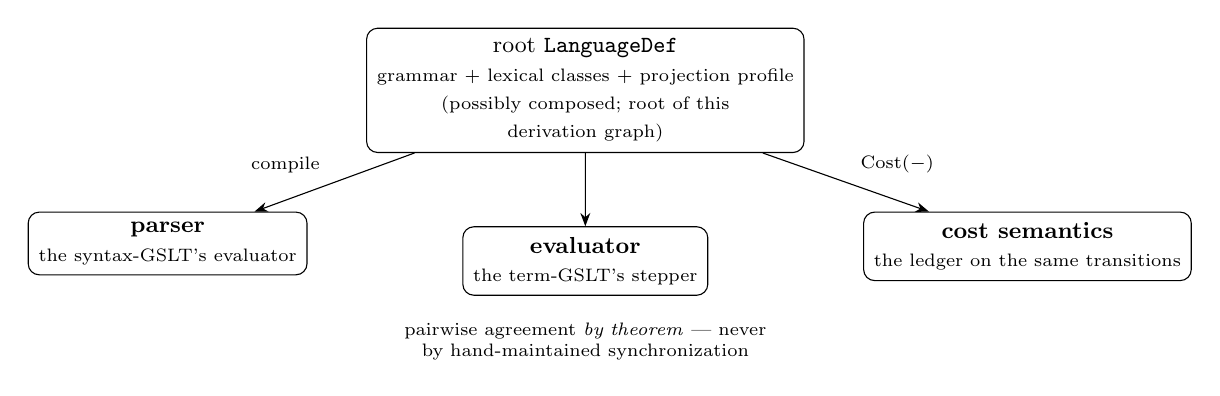
\begin{tikzpicture}[scale=0.93, transform shape,
  box/.style={draw, rounded corners, align=center, inner sep=4pt,
    font=\small}]
\node[box] (root) {root \code{LanguageDef}\\
  {\scriptsize grammar $+$ lexical classes $+$ projection profile}\\
  {\scriptsize (possibly composed; root of this}\\
  {\scriptsize derivation graph)}};
\node[box, below left=8mm and 8mm of root] (parser)
  {\textbf{parser}\\{\scriptsize the syntax-GSLT's evaluator}};
\node[box, below=10mm of root] (eval)
  {\textbf{evaluator}\\{\scriptsize the term-GSLT's stepper}};
\node[box, below right=8mm and 8mm of root] (cost)
  {\textbf{cost semantics}\\{\scriptsize the ledger on the same
    transitions}};
\draw[-{Stealth}] (root) -- (parser)
  node[midway, above left, font=\scriptsize]{compile\;};
\draw[-{Stealth}] (root) -- (eval);
\draw[-{Stealth}] (root) -- (cost)
  node[midway, above right, font=\scriptsize]{\;$\mathrm{Cost}(-)$};
\node[below=2.5mm of eval, font=\scriptsize, align=center, text width=6cm]
  {pairwise agreement \emph{by theorem} --- never by hand-maintained
   synchronization};
\end{tikzpicture}
\end{center}

\noindent
The compositional discipline is enforced starvation: no derived component
has any information channel back to the language except the proved
interfaces, so there is nothing left \emph{to} drift.  The formal side lives in the
Mettapedia Lean development and is sorry- and axiom-clean across the
roughly fifteen-thousand-line module family; the axiom reports below were
re-checked against the kernel when this section was first written.  The pipeline, for
the Metamath instance:

\begin{center}
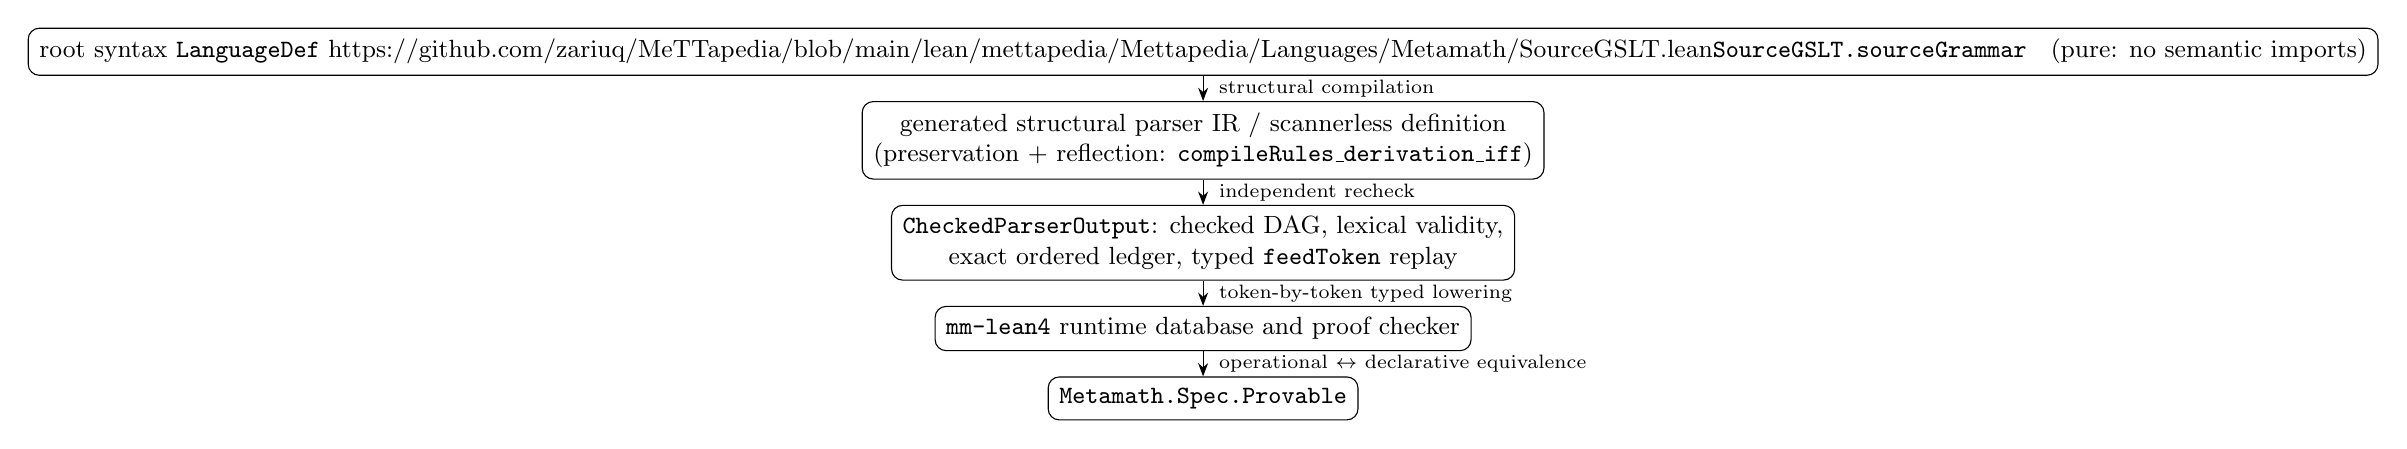
\begin{tikzpicture}[node distance=3.2mm,
  box/.style={draw, rounded corners, align=center, inner sep=4pt,
    font=\small}]
\node[box] (root) {root syntax \code{LanguageDef}
  \href{https://github.com/zariuq/MeTTapedia/blob/main/lean/mettapedia/Mettapedia/Languages/Metamath/SourceGSLT.lean}{\code{SourceGSLT.sourceGrammar}}
  \; (pure: no semantic imports)};
\node[box, below=of root] (ir) {generated structural parser IR / scannerless
  definition\\ (preservation $+$ reflection:
  \code{compileRules\_derivation\_iff})};
\node[box, below=of ir] (cert) {\code{CheckedParserOutput}: checked DAG,
  lexical validity,\\ exact ordered ledger, typed \code{feedToken} replay};
\node[box, below=of cert] (mm) {\code{mm-lean4} runtime database and proof
  checker};
\node[box, below=of mm] (spec) {\code{Metamath.Spec.Provable}};
\draw[-{Stealth}] (root) -- (ir)
  node[midway,right,font=\scriptsize]{\;structural compilation};
\draw[-{Stealth}] (ir) -- (cert)
  node[midway,right,font=\scriptsize]{\;independent recheck};
\draw[-{Stealth}] (cert) -- (mm)
  node[midway,right,font=\scriptsize]{\;token-by-token typed lowering};
\draw[-{Stealth}] (mm) -- (spec)
  node[midway,right,font=\scriptsize]{\;operational $\leftrightarrow$
    declarative equivalence};
\end{tikzpicture}
\end{center}

\noindent
Parsing and checking remain separate judgments at every stage; the
composition modules join them by theorem.  Generically, the same chain
reads as a sequence of seams, each crossed only inside a certificate:

\begin{center}
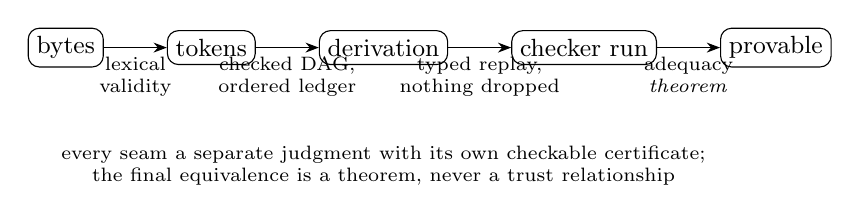
\begin{tikzpicture}[node distance=8mm,
  st/.style={draw, rounded corners, inner sep=3pt, font=\small}]
\node[st] (b) {bytes};
\node[st, right=of b] (t) {tokens};
\node[st, right=of t] (d) {derivation};
\node[st, right=of d] (c) {checker run};
\node[st, right=of c] (p) {provable};
\draw[-{Stealth}] (b) -- (t)
  node[midway, below, font=\scriptsize, align=center]{lexical\\ validity};
\draw[-{Stealth}] (t) -- (d)
  node[midway, below, font=\scriptsize, align=center]{checked DAG,\\
    ordered ledger};
\draw[-{Stealth}] (d) -- (c)
  node[midway, below, font=\scriptsize, align=center]{typed replay,\\
    nothing dropped};
\draw[-{Stealth}] (c) -- (p)
  node[midway, below, font=\scriptsize, align=center]{adequacy\\
    \emph{theorem}};
\node[below=9mm of d, font=\scriptsize, align=center]
  {every seam a separate judgment with its own checkable certificate;\\
   the final equivalence is a theorem, never a trust relationship};
\end{tikzpicture}
\end{center}

\paragraph{The generic compiler and its two-sided correspondence.}  A
generic, language-agnostic compiler turns the grammar fragment of any
\code{LanguageDef} into structural parser rules.  Three theorems bound its
authority.  Changing any non-syntax field of the declaration cannot change
the generated rules (\code{compileRules\_eq\_of\_terms\_eq}); generated-rule
actions retain the independently decoded terminal/child skeleton, so a rule
cannot silently drop, duplicate, or reorder children
(\code{compileRules\_action\_shape}); and --- the load-bearing result ---
derivability in the generated structural intermediate form is
\emph{equivalent} to derivability in the source grammar at the
ordered-token boundary (\code{compileRules\_derivation\_iff}: preservation
\emph{and} reflection, a genuine second relation rather than equality by
definition; kernel axioms exactly \code{propext},
\code{Classical.choice}, \code{Quot.sound};
\href{https://github.com/zariuq/MeTTapedia/blob/main/lean/mettapedia/Mettapedia/GSLT/Parsing/LanguageDefSyntaxCorrespondence.lean}{\code{GSLT/Parsing/LanguageDefSyntaxCorrespondence.lean}}).

\paragraph{Checked languages: two laws, crowns for free.}  The reusable
\code{CheckedLanguage} interface packages what any language must supply to
close the loop from bytes to meaning: a syntax-only root, a lexical
relation, a lowering into a checker, and a declarative judgment, subject to
exactly two laws --- exact lowering and checker adequacy.  From those two
laws the certificate-indexed and whole-pipeline crown theorems
(\code{pipelineAccepts\_iff\_parserAccepts\_and\_declarative} and kin) are
derived \emph{once, generically}; the generic composition layer
(\href{https://github.com/zariuq/MeTTapedia/blob/main/lean/mettapedia/Mettapedia/GSLT/CheckedLanguage.lean}{\code{GSLT/CheckedLanguage.lean}})
proves them with \emph{no axioms at all}.  Parsing and checking remain
separate judgments throughout: the composition joins them by theorem, and
neither the parser nor its certificate is ever allowed to authorize a
theorem.

\begin{center}
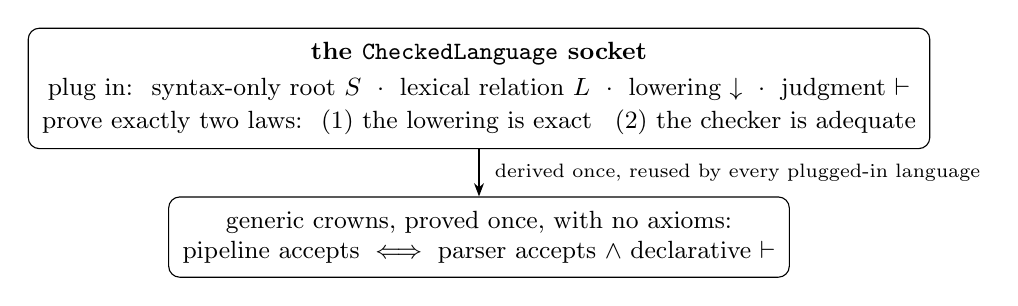
\begin{tikzpicture}[
  box/.style={draw, rounded corners, align=center, inner sep=5pt,
    font=\small}]
\node[box] (socket) {\textbf{the \code{CheckedLanguage} socket}\\[2pt]
  plug in:\; syntax-only root $S$ \;$\cdot$\; lexical relation $L$
  \;$\cdot$\; lowering $\downarrow$ \;$\cdot$\; judgment $\vdash$\\[1pt]
  prove exactly two laws:\; (1) the lowering is exact
  \;\;(2) the checker is adequate};
\node[box, below=6mm of socket] (crown)
  {generic crowns, proved once, with no axioms:\\
   pipeline accepts $\iff$ parser accepts $\wedge$ declarative $\vdash$};
\draw[-{Stealth}] (socket) -- (crown)
  node[midway, right, font=\scriptsize]
  {\;derived once, reused by every plugged-in language};
\end{tikzpicture}
\end{center}

\noindent
The expensive theorem is proved once, about the socket; each further
language pays only its own two laws.  That, rather than any property of
Metamath itself, is why the Metamath instance below is a template.

\paragraph{The Metamath vertical slice: a parser-to-provability crown.}
The first full instance runs from raw Metamath bytes to formal
provability.  The root Metamath syntax \code{LanguageDef} is a \emph{pure} grammar
--- a semantic firewall: it imports only the generic grammar-inference
layer, and the generic compiler contains no Metamath-specific names.  On
top of it, \code{CheckedParserOutput} demands an independently checked
grammar DAG, lexical validity, exact ordered-token agreement, and a
successfully constructed verified reader; \code{TypedLoweringCertificate}
pairs every classified source token, in order and without insertion or
omission, with an actual \code{ParserState.feedToken} transition of the
verified \code{mm-lean4} checker, and proves that the instrumented
execution erases to the production checker database.  The crown
(\code{generatedParserAndCheckerAcceptance\_iff\_specProvability}) then
states that generated-parser-plus-checker acceptance is equivalent to
declarative acceptance by \code{Metamath.Spec.Provable} --- kernel axioms
again exactly \code{propext}, \code{Classical.choice}, \code{Quot.sound}.
The reverse direction cannot manufacture syntax evidence: it is indexed by
an existing checked parser output whose certificates have already passed
their independent checkers.  The crown, verbatim from
\href{https://github.com/zariuq/MeTTapedia/blob/main/lean/mettapedia/Mettapedia/Languages/Metamath/SourceGSLTCheckerAlignment.lean}{\code{SourceGSLTCheckerAlignment.lean}}:

\begin{lstlisting}
def GeneratedParserAndCheckerAccepts
    {bytes : ByteArray} (output : CheckedParserOutput bytes)
    (label : String) (formula : Metamath.Verify.Formula) : Prop :=
  TypedLoweringCertificate bytes output.source /\
    ImplementationAccepts bytes label formula

theorem generatedParserAndCheckerAcceptance_iff_specProvability
    {bytes : ByteArray} (output : CheckedParserOutput bytes)
    (label : String) (formula : Metamath.Verify.Formula) :
    GeneratedParserAndCheckerAccepts output label formula <->
      DeclarativeAccepts bytes formula
\end{lstlisting}

\noindent
Executable closure evidence: seven checked
ordered ledgers (demo0, MIU, Peano, disjoint-variable and proof-format
cases, and an authentic propositional \code{set.mm} slice) in exact
object-level agreement with independent \code{mm-lean4} output;
normal/compressed proof agreement; five malformed-source rejections;
killed mutations across labels, disjoint-variable conditions, compressed
proofs, declaration order, AST, lexer, and semantic references; and
byte-identical regeneration of both generated Metamath artifacts from the
Lean root.

\paragraph{From parser-GSLT to checker-GSLT: source-owned inference.}
Since the vertical slice above was sealed, the same root \code{LanguageDef} has
grown a second semantic derivation: Metamath \emph{checking} itself as a
source-owned GSLT.
\href{https://github.com/zariuq/MeTTapedia/blob/main/lean/mettapedia/Mettapedia/Languages/Metamath/SourceGSLTOperations.lean}{\code{SourceGSLTOperations.lean}}
is the single declared bridge from the source grammar to the streaming
fold and indexed-checker operations: node contracts are \emph{computed}
from the parameter sorts of the source productions, and lexical references
resolve through the same literal tables that generate the parser.
\href{https://github.com/zariuq/MeTTapedia/blob/main/lean/mettapedia/Mettapedia/Languages/Metamath/SourceGSLTState.lean}{\code{SourceGSLTState.lean}}
gives those operations their scoped-state semantics (frames, scope
closing, global object identities) with no reference to the
\code{mm-lean4} runtime database, and
\href{https://github.com/zariuq/MeTTapedia/blob/main/lean/mettapedia/Mettapedia/Languages/Metamath/SourceGSLTNormalTheorem.lean}{\code{SourceGSLTNormalTheorem.lean}}
admits a normal-theorem transition only through an exact source-owned
proof-occurrence tree over the pre-insertion database prefix ---
independent of the \code{mm-lean4} execution function.  Operational and
declarative adequacy
(\code{SourceInferenceOperationalAdequacy},
\href{https://github.com/zariuq/MeTTapedia/blob/main/lean/mettapedia/Mettapedia/Languages/Metamath/SourceInferenceDeclarativeAdequacy.lean}{\code{SourceInferenceDeclarativeAdequacy.lean}})
connect this source-derived checker semantics to Metamath's declarative
semantics with every database, frame, declaration, and disjointness
premise derived from the same validated source prefix; the crown
(\code{NormalTheoremStep.toSemanticProvable}) was re-verified for this
section at kernel axioms exactly \code{propext}, \code{Classical.choice},
\code{Quot.sound}, with the module family sorry-free.  Export modules
(\code{SourceGSLTParserExport}, \code{SourceGSLTOperationsMeTTaExport})
regenerate both engine-facing artifacts from the root, and a native
inference-staging consumer (\code{lib\_parse\_inference\_native}, with its
benchmark harness) carries the operations export into the engine.  The
Metamath instance is thereby the template the programme intends to
replicate: \emph{one} root \code{LanguageDef} from which the parser, the checker
operations, and their adequacy theorems are all derived, ready to be
instantiated across a curriculum of further language definitions.

\paragraph{Declaration-level co-evolution with the shipped checker
(August 2026).}  The source-owned semantics above has since been joined to
the verified implementation at the level of individual transitions.  Every
accepted source declaration step --- \code{\$c}, \code{\$v}, \code{\$d},
\code{\$f}, \code{\$e}, assertion insertion for \code{\$a}/\code{\$p}, and
scope push/pop/completion --- is now matched by the \emph{shipped}
\code{mm-lean4} database operation it corresponds to (the per-token
declaration inserts, the checked hypothesis insertion, the axiom insertion
including its mandatory-frame trim), and the whole statement fold co-evolves
with the implementation database from the initial states with no supplied
premises (\code{default\_initial\_applyPayloads} in
\code{SourceGSLTRuntimeCoEvolution.lean}).  Two identifications carry the
weight: the implementation's mutable mandatory-frame computation is proved
equal to the specification's mandatory frame
(\code{trimFrame'\_eq\_mandatory}), and the accepted pipeline's own
classified stream supplies its lexical evidence
(\code{runSource\_selfLexicalized\_derives}), so neither the frame nor the
token boundary is ever assumed.  A deliberate honesty distinction
structures the remaining work: results proved from one accepted source run
and one checked byte representation are kept as \emph{parallel} certificates
until the classified stream is bound to the exact bytes the verified reader
consumed, each \code{\$p} obligation's normal or compressed proof is
discharged from the reader's own chronology (with verified and
incomplete-\code{?} outcomes as disjoint results), and the source fold is
related to the production reader by a prefix-wise simulation in which
reader microsteps are administrative and completed statements are the
observable steps.  The normal-proof discharge has been constructed against
the production reader trace; the compressed analogue and the whole-prefix
simulation are in active development.

\paragraph{Second consumers and the engine loop.}  Megalodon has an honest
second-consumer skeleton that reuses the generic signatures and crown ---
deliberately \emph{not} yet claimed as an instance, since its verified
checker and adequacy laws remain to be built.  On the engine side, the
generated Metamath grammar artifact is consumed directly by \CeTTa{}
(\code{lib\_parse\_metamath\_grammar\_generated\_v0.metta}) alongside the
\code{lib\_parse} family and the signature-driven ABT binder layer in the
Prime integration lane; the full engine-side parse gate (Metamath, ABT,
and native-reader tests) was re-run green for this section.  Honest
boundaries: the tested \code{set.mm} artifact is a nontrivial authentic
slice, not the full corpus; raw byte-to-token completeness is secured per
accepted certificate by exact typed reader replay, with a universal
raw-byte characterization theorem remaining future work; and the
declaration-level co-evolution above becomes a single bidirectional
statement only once the same-\code{LanguageDef} binding, per-\code{\$p}
discharge, and prefix simulation land, as itemized in the preceding
paragraph.

\subsection{\code{lib\_tptp}: standard formats around pluggable calculi}
\label{sec:lib-tptp}

TPTP is a family of standard problem and derivation formats, not a theorem
prover or a mandate for one proof-search strategy
\cite{tptp-language,tstp-derivations}.  This distinction determines the
library boundary.  \code{lib\_tptp} owns parsing, admitted semantic carriers,
format transformations, and derivation-DAG verification plumbing.  A
resolution or superposition searcher belongs in an example or an explicitly
named prover package; a TSTP rule belongs to a declared calculus service whose
soundness is checked independently.

\paragraph{The current native input boundary.}
The checked-in versioned TPTP \code{LanguageDef} generates a native ParserPack for
the official syntax family and a source-defined syntax-tree-to-abstract-syntax
projection.  The maintained MeTTa API exposes four useful stages:

\begin{itemize}
\item \code{tptp:file->syntax-tree};
\item \code{tptp:file->abstract-syntax};
\item \code{tptp:file->first-order-document};
\item \code{tptp:cnf-file->clause-data}.
\end{itemize}

Each returns an explicit stage value or stage fault, and each published value
is admitted against its own \code{LanguageDef}; no result is recast as a
legacy \code{ATPInput}.  The syntax gate includes representative TPI, THF,
NHF, TFF, NXF, TCF, FOF, CNF, include, annotation, numeric, Unicode, and
source-span cases.  For example:

\begin{lstlisting}[language={},caption={Representative inputs accepted by the versioned TPTP grammar}]
thf(identity,axiom,![P:$o]:(P=>P)).
tff(typed,axiom,![X:$i]:q(X)).
fof(first_order,axiom,![X]:(p(X)=>?[Y]:q(Y))).
cnf(clause,axiom,p(X)|~q(X)).
include('Axioms/SET003+0.ax',[first_order]).
\end{lstlisting}

\noindent
Parsing all of these families is not a claim that all of their semantics are
already implemented.  The deeper admitted transformation surface is
currently first-order FOF/CNF.  The four-profile executable gate checks the
public examples under Prime, PeTTa, HE-extended, and HE-prime; the umbrella
target also checks artifact-digest closure and mutations that remove or alter
load-bearing generated rules.

\begin{center}
\resizebox{\textwidth}{!}{%
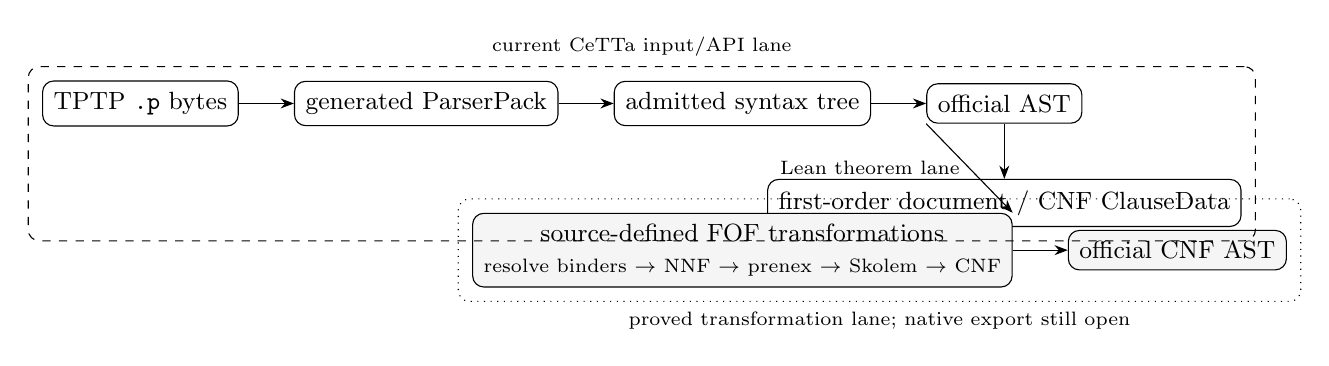
\begin{tikzpicture}[node distance=5mm,
  box/.style={draw, rounded corners, align=center, inner sep=4pt,
    font=\small},
  proof/.style={draw, rounded corners, align=center, inner sep=4pt,
    font=\small, fill=gray!8}]
\node[box] (bytes) {TPTP \code{.p} bytes};
\node[box, right=7mm of bytes] (pack) {generated ParserPack};
\node[box, right=7mm of pack] (tree) {admitted syntax tree};
\node[box, right=7mm of tree] (ast) {official AST};
\node[box, below=7mm of ast] (data) {first-order document / CNF ClauseData};
\draw[-{Stealth}] (bytes) -- (pack);
\draw[-{Stealth}] (pack) -- (tree);
\draw[-{Stealth}] (tree) -- (ast);
\draw[-{Stealth}] (ast) -- (data);

\node[proof, below=11mm of tree] (fof) {source-defined FOF transformations\\
  {\scriptsize resolve binders $\to$ NNF $\to$ prenex $\to$ Skolem
   $\to$ CNF}};
\node[proof, right=7mm of fof] (cnfast) {official CNF AST};
\draw[-{Stealth}] (ast.south west) -- (fof.north east)
  node[midway,left,font=\scriptsize]{Lean theorem lane};
\draw[-{Stealth}] (fof) -- (cnfast);

\node[fit=(bytes)(pack)(tree)(ast)(data), draw, dashed, rounded corners,
  inner sep=5pt, label={[font=\scriptsize]above:current \CeTTa{} input/API lane}] {};
\node[fit=(fof)(cnfast), draw, dotted, rounded corners,
  inner sep=5pt, label={[font=\scriptsize]below:proved transformation lane;
  native export still open}] {};
\end{tikzpicture}%
}
\end{center}

\paragraph{FOF-to-CNF as a compositional pipeline.}
On the theorem side, official FOF elaborates into named FOF, resolves to a
locally nameless binder representation, normalizes to NNF and prenex form,
Skolemizes with explicit generated-symbol evidence, introduces definitional
names, creates source-indexed clause batches, allocates collision-free TPTP
names, and serializes to the official CNF AST.  Each arrow is a declared
GSLT with an independent recursive semantics and exact agreement/no-invention
theorems.  The composed \code{endToEndExact\_exists} theorem obtains a
serializer result for every evidence-bearing admitted batch.  It does
\emph{not} yet produce concrete text; canonical printing and the
parser/printer round trip remain the next format boundary.

The shadowing fixture

\begin{lstlisting}[language={}]
fof(shadowing,axiom,![X]:(p(X)=>?[X]:q(X))).
\end{lstlisting}

\noindent
is the capture-avoidance canary: \code{q(X)} resolves to the inner binder.
Malformed numeric applications, unallocated variables, duplicate lexical
keys, and generated/original symbol collisions are rejected by negative
theorems rather than repaired by the serializer.

\paragraph{TSTP verification through a compact word language.}
The first logically closed profile accepts this ordinary ground-resolution
derivation:

\begin{lstlisting}[language={},caption={The ground TSTP canary}]
cnf(p_or_q,axiom,p|q).
cnf(not_p,axiom,~p).
cnf(not_q,axiom,~q).
cnf(q,plain,q,inference(resolution,[status(thm)],[p_or_q,not_p])).
cnf(empty,plain,$false,
    inference(resolution,[status(thm)],[q,not_q])).
\end{lstlisting}

\noindent
Admission retains node identity, roles, source annotations, parent order,
and \code{status(thm)}.  A status-indexed projection produces the semantic
program.  A generic compiler replaces formulas, rules, evidence, provenance,
obligations, and the finite service state with proof-local arena references
and seven compact records.  Decoding those words recovers the exact semantic
program.  A shared execution invariant then supplies a continuous trace in
the actual derivation-word \code{LanguageDef}, and the selected
ground-resolution service's independent soundness theorem turns its verified
empty root into unsatisfiability.

\begin{center}
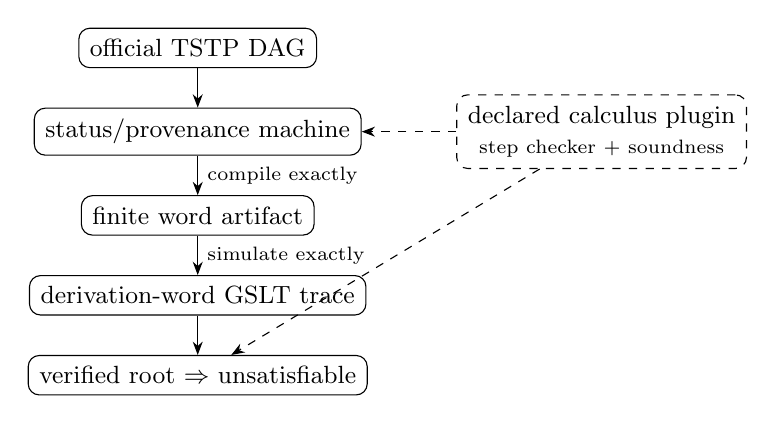
\begin{tikzpicture}[node distance=5mm,
  box/.style={draw, rounded corners, align=center, inner sep=4pt,
    font=\small},
  service/.style={draw, dashed, rounded corners, align=center,
    inner sep=4pt, font=\small}]
\node[box] (dag) {official TSTP DAG};
\node[box, below=of dag] (status) {status/provenance machine};
\node[box, below=of status] (word) {finite word artifact};
\node[box, below=of word] (gslt) {derivation-word GSLT trace};
\node[box, below=of gslt] (root) {verified root $\Rightarrow$
  unsatisfiable};
\node[service, right=12mm of status] (calculus)
  {declared calculus plugin\\
   {\scriptsize step checker $+$ soundness}};
\draw[-{Stealth}] (dag) -- (status);
\draw[-{Stealth}] (status) -- (word)
  node[midway,right,font=\scriptsize]{compile exactly};
\draw[-{Stealth}] (word) -- (gslt)
  node[midway,right,font=\scriptsize]{simulate exactly};
\draw[-{Stealth}] (gslt) -- (root);
\draw[-{Stealth},dashed] (calculus) -- (status);
\draw[-{Stealth},dashed] (calculus) -- (root);
\end{tikzpicture}
\end{center}

This design follows a maximal-native-calculus principle without hardcoding
resolution into \CeTTa{}: the graph/word machinery is calculus-neutral, while
each calculus supplies its most direct checker and semantic theorem.  The
current MeTTa resolution example deliberately begins only after
\code{lib\_tptp} has produced admitted ClauseData.  Its unification, bounded
search, trace object, and independent trace checker live together under
\code{examples/atp/tptp\_resolution}; neither search nor its local
\code{fo-proof} representation is a public TPTP API.

\paragraph{What remains before this is a native general TSTP verifier.}
The current closed theorem covers one ground \code{status(thm)} resolution
profile.  General TSTP support requires status-sensitive composition for
\code{thm}, \code{cth}, and \code{esa}; a registry of independently sound
calculus services; finite arenas for evolving service state; include-DAG
resolution; canonical concrete printing; E/Vampire ingestion and
reconstruction; and typed TFF/TCF/THF/NHF semantic carriers.  The word
checker must then be lowered by a source-defined transformation to StructuredC
with a commuting/reflection theorem.  Until that final step, the compact word
model is the proved native target shape, not a claim that the production C
implementation has been derived from it.

\subsection{MeTTa Zero: a two-operation kernel with native proof evidence}
\label{sec:zero-oslf-nik}

MeTTa Zero is the compact executable specimen for extending the preceding
programme from parsing to language semantics and compilation.  Assuming
s-expressions with variables, an occurrence bag $S$, matching with
substitution, and a declared grounding capability, its kernel has only two
public semantic operations.  Write $v$ for a fresh wildcard and abbreviate
the interpreted result bag by $R_S(x)$:

\begin{align}
\mathsf{query}_S(p,t)
  &= \biguplus_{a\in S}
       \{\,t\theta \mid \theta\in\mathsf{match}(p,a)\,\},
       \label{eq:zero-query}\\
R_S(x)
  &= \left(\biguplus_{(=\,l\,r)\in\mathsf{query}_S(v,v)}
       \{\,r\theta \mid \theta\in\mathsf{match}(l,x)\,\}\right)
       \uplus \mathsf{ground}(x),
       \label{eq:zero-results}\\
\mathsf{eval}_S(x)
  &= \begin{cases}
       R_S(x), & R_S(x)\neq\varnothing,\\
       \{x\},  & R_S(x)=\varnothing.
     \end{cases}
     \label{eq:zero-eval}
\end{align}

Equations are therefore ordinary queryable atoms, not entries in a private
rule store; evaluation obtains them through the same public query as user
programs.  Grounding is a declared library capability, and a capability's
decline leaves an uninterpreted subject inert rather than turning ignorance
into an empty result.  The coproducts are occurrence coproducts: duplicate
facts, rules, matches, and answers remain distinct.  A recursive semantic
runner, continuations, pending work, and \code{reify} compose over this
kernel; they are not silently folded into Equations~\ref{eq:zero-query}--
\ref{eq:zero-eval}.  The current runner is consequently retained as a
versioned experimental profile while its abstract laws and cross-dialect
interpretations are established.

\paragraph{One semantic root, three derived uses of native types.}
The Lean development sends Zero's actual composed
\code{ExtendedLanguageDef} and relation environment through OSLF, rather
than constructing a parallel transition relation:

\begin{center}
$\text{Zero language definition}
  \longrightarrow \text{relation-backed OSLF span}
  \longrightarrow \text{native types and certificates}$
\end{center}

\noindent
The resulting information has three distinct, proved uses.

\begin{enumerate}
\item \textbf{Spatial classification.}  Generated headed types recognize
  equation atoms and the exact query/evaluation request and answer
  constructors.  The constructor list is generated from the language's term
  grammar rather than maintained as a second inventory.
\item \textbf{Behavioral evidence.}  Exact query and evaluation diamond
  theorems identify the OSLF diamond with existence of an answer in the
  corresponding Zero occurrence bag.
  Proof-relevant finite certificates are sound and complete for this
  admitted fragment.  Generic predecessor-universal \code{box} evidence
  deliberately fails closed until finite predecessor enumeration, an
  invariant, or coinductive evidence is supplied.
\item \textbf{Compilation analysis.}  Constructor/arity head signatures
  select the query or evaluation production without inspecting every rule.
  Unsupported forms take the complete rule-table fallback.  The selected
  plan is proved equal both to the generic executor and to the source
  Zero interpreter under the exact occurrence-bag observer
  (\code{executeAuthoredNativePlanned\_eq},
  \code{nativePlanned\_eq\_authored}).  Thus the analysis establishes a
  safe shape for generated native dispatch; exporting that index into the
  C plan ABI is an implementation step, not a new semantic decision.
\end{enumerate}

The distinction between the second and third uses is load-bearing.  A
diamond records that at least one suitable transition exists; it does not
record how many occurrences produced it.  The negative theorem
\code{diamond\_equal\_but\_edge\_counts\_differ} exhibits two spans with
the same diamond observation and different edge multiplicities.  Native
types may therefore guide dispatch and justify existence claims, but they
cannot replace Zero's bag observer.

The generic native-type construction is in
\href{https://github.com/zariuq/MeTTapedia/blob/main/lean/mettapedia/Mettapedia/GraphTheory/Walk/NativeTypeTheory.lean}{\code{GraphTheory/Walk/NativeTypeTheory.lean}};
the concrete Zero theorems are in
\href{https://github.com/zariuq/MeTTapedia/blob/main/lean/mettapedia/Mettapedia/Languages/MeTTa/MeTTaZeroLanguageAdequacy.lean}{\code{MeTTaZeroLanguageAdequacy.lean}}.

\paragraph{From a trace to an independently replayed proof.}
CertificateGSLT's open derivations now carry an ordered context of explicit
premises, with a generic semantic-induction theorem: if every local rule
application preserves meaning and every open premise has its declared
meaning, the derived conclusion has its meaning.  Zero instantiates this
interface with one admitted \code{LanguageDef} of spatial rules and two
behavioral liveness rules, one for query rows and one for evaluation rows.
A liveness rule cannot mint an answer edge
by itself; it requires a query-row or evaluation-row premise tied to an
actual occurrence in the interpreted Zero relation.

A generic waist
(\href{https://github.com/zariuq/MeTTapedia/blob/main/lean/mettapedia/Mettapedia/OSLF/Framework/OSLFCertificateGSLTAuthority.lean}{\code{OSLF/Framework/OSLFCertificateGSLTAuthority.lean}})
turns an accepted open \code{WireArticle} into semantic authority for any
OSLF-generated native type system, and Zero specializes it to its MIK
authority, exposing the corresponding checked-lowering obligation for a native
NIK.  A positive article plus its true row premise entails the OSLF behavioral
claim (\code{sample\_article\_semantic}); the negative canary changes the
article's premise reference to an out-of-range occurrence and is rejected
(\code{sample\_wrong\_premise\_rejected}).  This is proof-producing compilation structure,
not merely a diagnostic trace.

\paragraph{The current C boundary.}
The executable Zero compiler separately emits a deterministic, hash-linked
build certificate for

\begin{center}
$\text{source LanguageDefs}\longrightarrow
  \text{admitted rules}\longrightarrow
  \text{CGP1 plan}\longrightarrow
  \text{generated C/H bytes}$.
\end{center}

\noindent
An independent build-time C checker rereads the sources, replays admission,
compares every compiled rule structurally, and checks the exact generated
artifacts; tampering and nondeterministic regeneration are gated.  This
checker is not linked into the ordinary \CeTTa{} executable, so normal
execution pays no certificate-parsing or trace-retention cost.  The claim is
nevertheless bounded: the certificate proves structural chain of custody,
not yet that executing CGP1 or the generated C realizes all declared Zero
observations.  The open row premises above are not yet closed by
authenticated C execution receipts, and the C checker is not yet generated
from the single CertificateGSLT acceptance predicate.  These are the remaining
seams between the working build attestation and end-to-end NIK replay.  The
C checker is independent of the Python producer, but deliberately reuses the
generic C parser, admission path, and plan decoder; the resulting common-mode
boundary is another reason the CertificateGSLT replay correspondence remains
necessary.

%% ────────────────────────────────────────────────────────────────────
\section{Related Work}
\label{sec:related}

\paragraph{Concurrent constraint programming.}
Saraswat et al.~\cite{saraswat1988} established the theoretical
framework for detecting stable properties of networks in concurrent
logic programming languages.  Their cc($\downarrow$,$|$) language,
with Tell/Ask on shared variables over a monotonic constraint store,
provides the semantic model that most closely matches \HE{}/\CeTTa{}'s
\code{match~\&self} evaluation.  The distinction between monotonic
constraint stores and independent-scope evaluation (Flat Concurrent
Prolog) precisely characterizes the semantic boundary between \HE{} and
\PeTTa{}.

\paragraph{Coordination and the interaction basis.}
The commit of Section~\ref{sec:interaction} is a double-pushout rewrite with
application conditions in the sense of algebraic graph
transformation~\cite{ehrig-agt}, specialized to bags of occurrences.  Its
derived forms recover the classic coordination languages: Linda's tuple
space~\cite{linda}, where \code{in} is a take and \code{rd} a keep;
Constraint Handling Rules~\cite{chr}, whose simplification and propagation
rules are takes and keeps with a history read as absence; the join
calculus~\cite{join-calculus}, whose join patterns are multi-take commits on
one location; software transactional memory~\cite{stm}, whose \code{retry}
parks a commit on what it read and whose \code{orElse} is an ordered choice;
and the reflective rho calculus~\cite{rho2005}, whose COMM is two takes.  What
the basis adds to these is a single form in which predicate queries are a separate,
declared part with their own stability discipline, and in which the laws a
region enjoys follow from the rights others lack there.

\paragraph{Incremental computation.}  The revision tokens of
Section~\ref{sec:nondet-state} follow the dependency-tracking shape of Salsa,
rustc's query system, build systems \`a la carte, Adapton and differential
dataflow~\cite{salsa-red-green,rustc-red-green,build-systems-carte,adapton,differential-arrangements},
coarsened to what MeTTa's occurrence identities and translation stages need.

\paragraph{MeTTa ecosystem.}
The MeTTaIL boot compilation pipeline~\cite{mettail} provides a
contract-first, Lean-backed compilation path for MeTTa stdlib modules,
complementing \CeTTa{}'s direct evaluation approach.  The Mettapedia
formalization project provides the Lean specifications (\code{EvalSpec},
\code{MeTTaEval}, \code{MatchSpec}) that ground both the translation
proof and the \CeTTa{} evaluator design.  JeTTa compiles MeTTa to JVM
bytecode~\cite{jetta-slides,jetta-review}, and MORK runs the MM2 rewriting
language over \PathMap{} tries; both appear in this paper's comparisons.  The
PLN (Probabilistic Logic Networks) framework uses MeTTa's backward chaining
extensively; the typed chainer pattern from Nil Geisweiller's
\code{nilbc.metta} is the standard PLN idiom that works across all three
runtimes.

%% ────────────────────────────────────────────────────────────────────
\section{Conclusion}
\label{sec:conclusion}

\CeTTa{} is now one binary for several MeTTa dialects, each a named semantic
product with its own oracle.  The listings of Section~\ref{sec:tutorial} show
both what the dialects share and where they differ, and the differences are
principled: inert data against Prolog failure, argument types that decide
evaluation, call by need, and an editable standard library.  The semantics is
kept honest by result-bag conformance against upstream \HE{} and
SWI-\PeTTa{}, by a reflective modal layer, and by a rule table whose removal
tests show the evaluator depends on its declared rules.

The lines of development divide the work.  \code{main} is the published
baseline of August.  Opt does the careful fixes: in October it realized
\code{transform} natively over its MeTTa library, made space drains linear,
brought the cost of crossing between machines toward the cost of an ordinary
step, and, in staged work, runs an MM2 application suite as MeTTa faster than
MORK.  Pre-main unifies execution across the machines behind one call and
return contract, as the candidate for the next \code{main}.  The NIK line
grew native kernels and native application libraries.  The Prime draft
develops Prime in C in step with its metatheory, has absorbed the weights,
cost and parallel line and \code{cetta-ours}, and runs the interaction basis
as a native kernel.  The measured results are honest in both directions:
\CeTTa{}'s \PeTTa{} lane is clearly faster than SWI-\PeTTa{} on most of a
96-cell panel and still slower on foreign-data reads, the chainer cells, the
Ambient program and a rho cell; the Prime lane is the slow one, and its need
machinery is the cost.

For spaces and channels the direction is one interaction form.  Its theory is
largely proved; its surface runs in the Prime draft; its native runtime, with
stable occurrence identities, per-occurrence claims, per-region epochs and a
wait index, is the main thing still to build.

\paragraph{Remaining work.}
\begin{itemize}
\item \textbf{Opt.} Commit the staged join work; commit the checked spread
  hash, so that two representations of the empty list are one atom to
  \code{unique-atom}; make \code{remove-atom} of a bare symbol remove it;
  clear the three timing holds; and close the remaining SWI-\PeTTa{} wins.
\item \textbf{Pre-main.} Commit the staged repairs, run the exhaustive
  \code{main} qualification, and advance \code{main}.
\item \textbf{Prime draft.} Repair the deviations of
  Section~\ref{sec:prime-draft}, with the weights line repairing its thirteen
  fixtures; make the occurrence kernel the single engine for \code{transform}
  on both lanes; build the native runtime of the interaction basis; and close
  the authority gaps: ticket requirements that a child grant may drop, names
  that confer their holder's rights, and an effect capability in place of the
  evaluator's thread-local flag.
\item \textbf{\HE{} one-step certification.} Certify the five live rules that
  are still bag-tested (\code{let}, \code{let*}, \code{case}, \code{switch},
  \code{switch-minimal}), through the matcher bridge of
  Section~\ref{sec:rulecert}, and carry the ground-query adequacy result to
  queries that contain variables.
\item \textbf{Zero native kernel closure.} Generate the native checker from the
  one CertificateGSLT acceptance predicate, authenticate query-row and
  capability receipts, and compose the build certificate with an execution
  receipt.
\item \textbf{Reaction semantics.} Extend the witness-free characterization of
  evaluation at communication to concurrent and persistent reactions.
\end{itemize}


\appendix

%% ════════════════════════════════════════════════════════════════════
\section{How the Listings Were Run}
\label{app:runs}

Every listing and probe in Section~\ref{sec:tutorial}, and every probe quoted
in Sections~\ref{sec:specdriven}, \ref{sec:interaction} and~\ref{sec:prime},
was run on 27 October 2026 with the binaries below, each from the working
state of its tree (which includes uncommitted changes) and each run in place,
because a \CeTTa{} binary finds its libraries relative to its own location.
A binary is named by the first twelve hexadecimal digits of the SHA-256 digest
of its file; the digests were taken before the runs and again after them, and
did not change.

\begin{center}
\footnotesize
\begin{tabular}{@{}p{0.25\linewidth}p{0.47\linewidth}p{0.20\linewidth}@{}}
\toprule
used for & binary (version, build date) & SHA-256, tree head \\
\midrule
\HE{} and \PeTTa{} lanes; rho calculus & \code{cetta} of the pre-main worktree (1.5.0-dev, 26 Oct) & \code{1db746ecc1ec}, feba78e3 \\
Prime lane & the Prime draft's \code{cetta-interaction-basis-}\allowbreak\code{m5-20261027} (1.5.0-dev, 27 Oct) & \code{7b25fbd48cc0}, a0f1077a \\
Prime lane, second binary & the Prime draft's \code{cetta-draft-merges-}\allowbreak\code{20261027} (1.5.0-dev, 27 Oct) & \code{ee205ed7c764}, a0f1077a \\
runtime counters & the pre-main worktree's \code{cetta-main-runtime-stats} (1.5.0-dev, 25 Oct) & \code{54278a7df178} \\
the published \code{main} & \code{cetta} of the \code{main} checkout (1.4.0-dev, 21 Sep) & \code{a45d87417931}, 12da03b4 \\
SWI-\PeTTa{} & the \PeTTa{} reference checkout (1.0.6) on SWI-Prolog 10.1.9 & b74af1b \\
\bottomrule
\end{tabular}
\end{center}

\noindent
The \HE{} lane runs as \code{cetta -{}-lang he -{}-pretty-vars file}, the \PeTTa{}
lane as \code{cetta -{}-lang petta -{}-pretty-vars file}, the Prime lane as
\code{cetta -{}-lang prime -{}-pretty-vars file}, and SWI-\PeTTa{} through its
\code{run.sh} with \code{-{}-silent}.  The \code{transform} listing was run on
SWI-\PeTTa{} with the same library file imported by a relative path, because
\code{(library lib\_transform)} names a library shipped with \CeTTa{}; its
native and authored firings on \CeTTa{} differ only by the environment switch
\code{CETTA\_TRANSFORM\_REFERENCE=1}.  Timings quoted from these runs (startup,
\code{fib}, the \code{variant} table) are single whole-process runs on a
shared sixteen-core workstation, measured with \code{/usr/bin/time}, and are
indicative only.

\paragraph{Probes beyond the listings.}  The text also quotes these runs:
\begin{itemize}
\item the one-step reflection layer \code{lts:he} and the rule table
  (\code{lts:he:step-rules}), on the \HE{} lane with the extended profile;
\item untabled and tabled \code{fib 25} and \code{fib 30} on the \HE{},
  \PeTTa{} and Prime lanes, and on \code{main};
\item the Prime outcome, variable, held-data and \code{delay}/\code{resample}
  behaviour, and the draft deviations of Section~\ref{sec:prime-draft};
\item the closed $\lambda\Pi$ conformance files and the explicit
  need-control fixture of the Prime draft, compared with their expected
  outputs;
\item the rho cost examples of Section~\ref{sec:rho-cost}, compared with their
  expected outputs.
\end{itemize}

\appendix

\section{\LeaTTa{} Cross-Check Appendix}
\label{app:leatta}

\LeaTTa{} is a Lean~4 MeTTa runtime and proof development that is useful
as an independent semantic cross-check for the \HE{}-facing core of
\CeTTa{}.  The local checkout used for the measurements in this
appendix was a clean \LeaTTa{}~1.0.6 tree at
\href{https://github.com/MesTTo/LeaTTa}{\code{github.com/MesTTo/LeaTTa}},
commit
\href{https://github.com/MesTTo/LeaTTa/tree/51b4b52bd02745992448835f5173989baf1436b5}{\code{51b4b52}}
(\code{2026-06-22}, ``prepare~1.0.6 release'').  Upstream release
notes and the checked-claims book are published at
\href{https://mestto.github.io/LeaTTa/}{\code{mestto.github.io/LeaTTa/}}.

This appendix records a local scope-and-spot-check run on 2026-06-24; it
is a coverage map, not a new benchmark ladder replacing the main paper.
The \CeTTa{} side used \code{-{}-profile he-extended -{}-lang he}.  The
\LeaTTa{} side used \code{-{}-oracle} for assertion-bearing files and
\code{-{}-file} for pure loaders.  A bulk pass ran every \code{.metta}
file under the \CeTTa{} tree (1255 files) through \LeaTTa{}.

\paragraph{Coverage, in three tiers.}
The raw aggregate---168 of 951 assertion-bearing files passing in
full---is misleading on its own, because most of the \CeTTa{} test
corpus exercises extension builtins that \LeaTTa{}, a deliberately
minimal \HE{} interpreter, does not implement and is not meant to.  The
honest decomposition is:

\begin{center}
\small
\begin{tabular}{p{3.3cm}p{11.3cm}}
\toprule
Tier & What \LeaTTa{} does on it \\
\midrule
\HE{} core & \textbf{Strong.}  Of the 21 \code{he\_*} conformance files,
18 pass in full and 2 partially (one loader carries no assertions),
for 203/206 assertions.  Full passes span symbols, equal-chaining,
backchaining, GADTs, dependent types, higher-order functions, grounded
basics, type propagation, states, documentation, and PLN truth values.
This is the fragment that overlaps the \HE{} evaluation semantics. \\
\addlinespace
\CeTTa{} extensions & \textbf{Out of scope by design.}  The bulk of the
783 partial failures call builtins \LeaTTa{} does not provide:
MORK-backed spaces (84 files), \PathMap{} (44), \code{hyperpose} (27),
typed \code{new-space hash}/\code{queue} (12), \code{import!} (10),
\code{space-set-match-backend}, and the textual Metamath parser.
Failing these reflects \LeaTTa{}'s minimalism, not a fidelity gap. \\
\addlinespace
Genuine gaps & \textbf{In-scope divergences.}  A float-only numeric
model: \code{(min-atom (5 4 6))} returns \code{4.000000} rather than an
integer, and rationals such as \code{1/2} raise ``only numbers
allowed,'' so the exact integer/rational tower does not correspond.
Typed error contours (e.g.\ \code{(+ 5 "S")} $\to$ \code{BadArgType},
empty/wrong-arity \code{car-atom}/\code{decons-atom}/\code{min-atom})
are not reproduced; we treat these as accepted divergences.  Two
\code{he\_b4} assertions touching inert-symbol and empty-match
semantics, and the higher-order WM-PLN bridge (218/221 on this
checkout), remain to be diagnosed. \\
\bottomrule
\end{tabular}
\normalsize
\end{center}

\paragraph{Spec repair triggered by the cross-check.}
The \LeaTTa{} comparison was useful not only as an oracle but as a
debugger for our own \HE{} Lean formalization.  During this pass we found that
the public equation-query path had been routed through the simplified
\code{simpleMatch} helper even though the faithful two-sided
\code{matchAtoms}/\code{mergeBindings} semantics already existed.  The
repair is now written down in three Lean files:
\code{DeclMatchSpec.lean} gives a declarative specification of
\code{match\_atoms} and proves \code{matchAtoms\_sound}/\code{\_complete};
\code{DeclMergeSpec.lean} does the same for
\code{merge\_bindings}, proving \code{mergeBindings\_sound}/\code{\_complete};
and \code{QueryInterfaceAgreement.lean} proves the staged ground-fragment
adequacy theorems
\code{queryEquations\_ground\_two\_way\_adequate} and
\code{queryEquationsAgainstVisible\_ground\_two\_way\_adequate}.  So the
cross-check is now anchored on the faithful ground-query API rather
than on the older simplified one.  The remaining variable-bearing query
case is deliberately left explicit: it requires the next repair, namely
threading equalities through \code{Bindings.resolve}/\code{Bindings.apply},
and is the right next theorem rather than a hidden assumption.

\paragraph{Performance.}
On matched runs \LeaTTa{} is correct where it is in scope but slower and
markedly more memory-hungry than \CeTTa{}'s C runtime---operational
overhead expected of an executable Lean interpreter, not a semantic
limitation.

\begin{center}
\small
\begin{tabular}{p{4.2cm}p{2.1cm}p{2.1cm}p{5.9cm}}
\toprule
Benchmark & \CeTTa{} & \LeaTTa{} & Note \\
\midrule
tail\_recursion\_deep\_regression & 0.30\,s & 0.80\,s &
both pass 3/3 assertions \\
tail\_recursion\_deep & 0.30\,s & 0.80\,s &
both pass 3/3 assertions \\
he\_c3\_pln\_stv & 0.10\,s & 0.10\,s &
both pass 5/5 assertions \\
he\_d2\_higherfunc & 0.10\,s & 0.10\,s &
both pass 25/25 assertions \\
test\_wmpln\_ho\_similarity\_bridge & 0.10\,s & 0.10\,s &
\CeTTa{} passes; \LeaTTa{} passes 218/221 assertions \\
bio\_refseq\_723k & 0.40\,s & 3.30\,s &
both run; \LeaTTa{} $\approx$1.16\,GB RSS vs.\ \CeTTa{} $\approx$196\,MB \\
bio\_tfbs\_415k & 0.30\,s & 2.10\,s &
both run; \LeaTTa{} $\approx$917\,MB RSS vs.\ \CeTTa{} $\approx$136\,MB \\
\bottomrule
\end{tabular}
\normalsize
\end{center}

\paragraph{Tilepuzzle: semantics vs.\ performance.}
The raw \CeTTa{} tilepuzzle benchmark depends on \CeTTa{}'s typed
\code{queue} and \code{hash} spaces, so it does not run unchanged on
\LeaTTa{} (a Tier-2 builtin mismatch).  A bounded adaptation replacing
those spaces with a functional queue and plain named-space membership
does run: a 100-step witness reaches 171 visited states in 18.47\,s,
while the 500-step version did not finish under a 30\,s cap.  For
reference, the clarified native contract counts
181{,}440 reachable states including the start board, while the older
\PeTTa{} example's 181{,}441 self-check is a counter-convention
difference, not evidence for an extra reachable board.  A fresh full
native \CeTTa{} run now completes with the tail-safe evaluation-arena
garbage collector:
181{,}440 states in 8.80\,s at 233\,MiB (Section~\ref{sec:tilepuzzle-gc}).
So this bounded \LeaTTa{} adaptation is only evidence that the algorithmic
idea transfers, while the full native \CeTTa{} row is settled capacity
evidence.

\paragraph{Bottom line.}
\LeaTTa{} is a credible independent oracle and a candidate verified
engine-floor for the \HE{} evaluation core of \CeTTa{}: it agrees on the
conformance set that matters, diverges only on extension builtins it
deliberately omits and on a float-only numeric model, and pays an
expected interpreter-speed cost.  Linking \LeaTTa{} to the \HE{} Lean
specification is therefore well-founded on the core, provided the
numeric tower and error-contour divergences are encoded as known
boundaries.  The specification side is now in a better state than when
this appendix was first drafted: the ground-query fragment is connected
to the faithful \HE{} matcher/merge semantics by proved two-way adequacy,
and the remaining variable-bearing query case has been isolated cleanly
enough to be attacked next rather than smudged into the oracle story.

%% ════════════════════════════════════════════════════════════════════
\section{\textsc{Experimental} --- MAM: The MeTTa Abstract Machine}
\label{app:mam}

\emph{This appendix is explicitly experimental.  It captures design
exploration from ongoing discussions (April~2026) between the authors
and external reviewers, concerning the
post-phase-1f abstract-machine layer for \CeTTa{}.  The original proposal is
retained because it records the design pressure, but the blanket statement
that nothing is implemented is no longer true: several machine components
landed during August~2026.  They do not yet constitute a final universal MAM,
and proposed names or categorical readings below remain revisable.}

\subsection{Motivation}

The phase-1f-era extraction seam (\code{src/search\_machine.\{h,c\}})
pulls policy parsing, stream combinators, and a \code{TableStore}
plugin out of \code{eval.c}, and wraps them in a thin callback struct
\code{CettaSearchMachine = \{stream\_source, eval\_bound\_single,
  eval\_ctx, table\_plugin\}}, stack-allocated at each call site.
This is a useful refactor, but it is a \emph{plug interface} — not an
abstract machine in the WAM / ZAM / SLG-WAM sense.  Real abstract
machines (XSB's SLG-WAM, SWI's tabling runtime, Soufflé's compiled
Datalog, miniKanren's CPS-transformed search) have persistent machine
state, explicit visitor protocols, capability advertisement, and
episode lifetimes.

The proposal here is a \emph{principled} next layer that retains the
current code as \code{SearchAdapter} (transitional helper) while
naming the real abstraction from first principles.

\subsection{Current categorical reading}

The MAM's present semantic reading, under active revision, models it
as a \textbf{quantale-enriched traced profunctor}, fibrated for
reflection.  This reading is provisional --- it captures the current
best understanding of the structure, not a definitional claim that
binds future architecture.  Unpacked:

\begin{itemize}
\item \textbf{Profunctor} $P : \mathcal{Q}^{\mathrm{op}} \times
  \mathcal{A} \to \mathcal{V}$: \emph{search}.  Queries in
  $\mathcal{Q}$ relate to answer streams in $\mathcal{A}$, with
  intensity weighted by elements of $\mathcal{V}$.
\item \textbf{Quantale enrichment} $\mathcal{V} = (L, \otimes, \le,
  \bigvee)$: \emph{multiplicity}.  Answer weights live in a quantale:
  $\mathcal{V} = \mathbf{2}$ for classical boolean search;
  $\mathcal{V} = \mathbb{N}$ for counted answers;
  $\mathcal{V} = [0,1]^2$ (strength $\times$ confidence) for PLN.
  \PathMap{}'s trie-algebra is natively a quantale.
\item \textbf{Trace} $\mathrm{Tr}_X^{A,B} : \mathrm{Hom}(A \otimes X, B
  \otimes X) \to \mathrm{Hom}(A, B)$: \emph{fixpoint}.  Feedback /
  saturation / tabling / cyclic queries are all instances of
  categorical trace (Joyal--Street--Verity, Hasegawa).
\item \textbf{Kleisli structure over an effect monad} (or algebraic
  effect handlers \emph{\`a la} Plotkin--Pretnar): \emph{control}.
  Demand, cut, suspension, resumption, and schedule are composable
  effect operations.
\item \textbf{Fibration} $p : \mathcal{T} \to \mathcal{B}$ (optional,
  for reflective MeTTa): rules-over-machine-state.
\end{itemize}

A trace operator is provably equivalent to taking the least fixpoint
of a parameterised endofunction (Hasegawa 1997); this is why tabling,
PLN-convergence, and saturation all fit one uniform operator.

\subsection{The proposed machine family: MAM}

We name the machine family \textbf{MAM: MeTTa Abstract Machine}.
The name is chosen by identity rather than by current structure or
scope: MAM is the abstract machine for the MeTTa language family,
and that identification remains accurate as the internal architecture
evolves.  The naming tradition (WAM, ZAM, STG, CEK, CAM) uses either
author identity or component decomposition; MAM uses the language
identity it serves, which is stable across architectural iteration.
Specifically, MAM does \emph{not} hardcode a categorical claim (as
``QAM = Quantale Abstract Machine'' would have done), and does
\emph{not} hardcode a functional scope (as ``SCAM = Search \& Control
Abstract Machine'' would have done).  The categorical reading and the
current feature set are both free to evolve without renaming.

\begin{center}
\begin{tabular}{ll}
\toprule
\textbf{Concept} & \textbf{Name} \\
\midrule
Machine family & \code{MAM} (MeTTa Abstract Machine) \\
Formal description & Quantale-enriched traced profunctor \\
Engine 1 (goal-directed, Kleisli/effect) & \code{Chainer} \\
\quad first realization (native) & \code{native\_chainer} \\
Engine 2 (fixpoint, trace) & \code{Saturator} \\
\quad first realization (pathmap) & \code{pathmap\_saturator} \\
Per-session state & \code{Episode} \\
Dispatch vtable & \code{MAMOps} \\
Answer & \code{Answer} / \code{WeightedAnswer} \\
Schedule axis & \code{dfs} / \code{bfs} / \code{iddfs} / \code{interleave} / \code{native} \\
Demand axis & \code{unbounded} / \code{once} / \code{limit-k} / \code{fold} \\
Visitor control & \code{CONTINUE} / \code{STOP} / \code{ERROR} / \code{SUSPEND} \\
\bottomrule
\end{tabular}
\end{center}

\subsection{The two-engine pressure strategy}

Rather than over-specifying a first concrete machine, MAM is
pressured from day~1 by \emph{two} independent realizations that
stress complementary axes of the seam:

\begin{description}
\item[\code{Chainer} (goal-directed).]  WAM-lineage control: explicit
  environments/frames, choicepoints, trail/undo, deterministic
  tail-path handling, bounded-demand response, direct conjunction
  when advertised.  Design-guide workload: \textbf{metamath backward
    chaining}.  Before the evaluation-arena garbage collector this
  workload could exhaust memory on \CeTTa{}; with the collector
  \CeTTa{} now completes the Metamath proof-search rows
  (Section~\ref{sec:benchmark-programs}), so the remaining motivation
  here is WAM-lineage control, not a memory-exhaustion gap.
  First realization: \code{native\_chainer}.
\item[\code{Saturator} (fixpoint).]  SLG / Datalog / saturation
  lineage: snapshots, delta-sets, conjunction planning, exact
  membership, counted answers, eventual path toward PLN and
  ATP-style saturation.  Design-guide workload: \textbf{PLN
    multi-pattern deduction}.  First realization: \code{pathmap\_saturator}
  (because \PathMap{}'s quantale structure makes weighted answer
  aggregation natural).
\end{description}

This pair creates the right kind of pressure on the seam: Chainer
forces frames, choicepoints, \code{EnvRef}, demand handling, and
explicit scheduling; Saturator forces snapshots, delta sets,
conjunction planning, exact membership, counted answers, and the
eventual path to PLN and ATP.

Compiled / bytecode (ZAM-lineage) and ATP saturation engines are
explicit \emph{later} lanes --- they risk freezing the protocol in
the wrong shape if pursued before Chainer and Saturator coexist
cleanly under one MAM.

\subsection{Axes that must stay separate}

A core architectural commitment is that the following axes are
\textbf{distinct data} in \code{SearchRequest}, not tangled behind
source-level operators:

\begin{description}
\item[Schedule.]  \code{dfs}~/~\code{bfs}~/~\code{iddfs}~/\code{interleave}
  are \emph{fairness policies}, not engines.  Korf's classic result
  motivates \code{iddfs} as a completeness-friendly default over raw
  \code{bfs} (BFS completeness with DFS memory); miniKanren's
  interleaving exists precisely to avoid starvation on infinite
  branches.
\item[Demand.]  \code{once}~/~\code{limit-k}~/~\code{unbounded}~/\code{fold}
  describes how many answers are requested, independently of schedule.
  \code{once} and \code{select~1} must build \code{demand = FIRST};
  they must \emph{not} silently hardcode DFS.
\item[Table mode.]  \code{none}~/~\code{variant}~/~\code{subsumptive}~/\code{incremental}
  mirrors the XSB / SWI ladder; each is an explicit engine-level choice.
\item[Backend.]  \code{native}~/~\PathMap{}~/~MORK chosen by the
  actual \code{Space}, not by a global preference.
\item[Lane.]  \code{recursive-dependent-proof}~/~\code{atp-saturation}~/\code{solver-oracle}~/~\dots{}
  chosen in source syntax.
\end{description}

The request builder (one per \code{-{}-lang}) normalizes concrete syntax
into \code{SearchRequest~+~SearchLangContract}; the MAM consumes the
normalized object, never raw source atoms.

\subsection{The seven-type vocabulary}

The original proposal used the following seven-type vocabulary.  The
implementation did not land this table literally: narrower, falsifiable
objects such as \code{PettaSearchMachine}, \code{MatchDecision},
\code{PreparedPureProgram}, and \code{RuleMachineCoreV1} emerged first.
The table remains a useful comparison vocabulary, not a frozen C ABI.

\begin{center}
\begin{tabular}{ll}
\toprule
\textbf{Type} & \textbf{Categorical role} \\
\midrule
\code{SearchRequest} & Object of $\mathcal{Q}$ \\
\code{SearchAnswer} & Object of $\mathcal{A}$ (quantale-weighted) \\
\code{SearchLangContract} & Subcategory inclusion $\mathcal{C} \hookrightarrow \mathrm{MAM}$ \\
\code{SearchCaps} & Capabilities = presence of morphisms/natural transformations \\
\code{VisitCtl} & Algebra of the effect operation $\mathrm{visit}$ \\
\code{MAMOps} & Kleisli dispatch vtable \\
\code{Episode} & One trace-iteration instance \\
\bottomrule
\end{tabular}
\end{center}

General implementation-level \code{SUSPEND/RESUME}, cancellation tokens,
backend-independent snapshot handles, and a single per-\code{-{}-lang} MAM
registration hooks remain deferred; individual machines already carry
narrower instances of several of these concerns.

\subsection{Implemented machine substrate (August 2026)}

The landed components answer several of the proposal's original questions
without pretending that one universal machine has been completed:

\begin{description}
\item[Choice and continuation ownership.]
  \code{PettaSearchMachine} owns an explicit heap of clause activations,
  environments, continuations, choice frontiers, binding rollback, and answer
  projection.  Its host callback API supplies language services but does
  not own the \PeTTa{} choice point.  \code{SearchContext} retains the small
  shared bindings/scratch save-and-rollback protocol.
\item[Revision-pinned candidate programs.]
  \code{MatchDecision} compiles sparse weak-head clause discrimination and
  callable caches under language, profile, language definition, compiler, and space
  identity.  It may omit only structurally impossible clauses and returns a
  candidate superset; selected open equations are standardized apart under a
  fresh epoch and rechecked by the authoritative matcher.  Indexing therefore
  cannot become binding authority.
\item[Prepared and compiled fragments.]
  \code{PreparedPureProgram} admits a deterministic, effect-free closed
  equation fragment with explicit heap control and conservative fallback.
  \code{RuleMachineCoreV1} executes bounded admitted rule packages and
  inspectable bytecode blocks under revision-pinned publication.  These are
  compiled fragments with mutation/staleness gates, not a claim that arbitrary
  MeTTa has been compiled.
\item[Observer-safe substitution fusion.]
  Ordinary clause activation previously traversed a result to apply its local
  substitution and then traversed it again for the enclosing environment.
  The current matcher can compose these substitutions and traverse once, but
  only when the host reports that the equation's result payload is not
  observed (today \code{equation\_result\_payload\_observed}).  If an observer
  may inspect the intermediate payload, the two-stage path remains
  authoritative.  Observer visibility, rather than benchmark identity, is the
  optimization license.
\item[Analysis-provider isolation.]
  The \PeTTa{} \code{typecheck-v2} profile enters through
  \code{PettaAnalysisService}, whose identity, ABI, policy, mutable authority,
  judgments, reasons, and ready-call validation are explicit.  The search
  machine no longer names the Roman-derived checker; a genuinely generic type
  and elaboration machine remains open.
\end{description}

The result is a family of interoperating machine components over shared term,
space, and observation contracts.  Compact activation environments,
mode/relation-indexed clause dispatch, generic tabling, and a unified episode
protocol remain structural work; the implementation evidence no longer
supports describing the whole layer as a mere callback proposal.

\subsection{Reference base}

The proposal draws on the following literature, all available in the
local library:

\begin{itemize}
\item \emph{A\"{\i}t-Kaci 1991, WAM Tutorial Reconstruction} --
  foundational WAM semantics; drives \code{Chainer} design.
\item \emph{Swift \& Warren, XSB System Manual; Sagonas et al.\ 1994} --
  SLG-WAM tabling; drives \code{Saturator} / table-mode ladder.
\item \emph{Scholz, Jordan, Suboti\'c, Westmann 2016, Soufflé: On Fast
  Large-Scale Program Analysis in Datalog (CC)} -- staged compilation
  of fixpoint computation; compiled \code{Saturator} path.
\item \emph{Keoliya \& Byrd 2020, microKanren} -- interleaving search
  as a distinct schedule axis.
\item \emph{Ager, Biernacki, Danvy, Midtgaard 2003, A Functional
  Correspondence Between Evaluators and Abstract Machines (BRICS)} --
  derivation methodology for machines from evaluator semantics.
\item \emph{Leroy 1990, The ZINC Experiment} -- machine-description
  vs.\ run-instance separation (maps to
  \code{MAMOps}~/~\code{MAM}~/~\code{Episode}).
\item \emph{Russell \& Norvig, AIMA Ch.~3} -- IDDFS completeness;
  uniform treatment of uninformed search.
\end{itemize}

\subsection{Status}

Since this appendix was first drafted, the derivation methodology it
cites has acquired kernel-checked foundations in the Mettapedia Lean
tree (\code{Mettapedia/Machines/}): a functional-correspondence module
deriving a CEK-shaped eager machine and a Krivine-shaped demand-driven
machine from fueled evaluators over one shared term substrate, with the
evaluator-to-machine correspondence and machine determinism proved; a
cone-duality module (forward/production and backward/demand reachability
cones, their Galois adjunctions, wavefront exhaustion, and the
demand-diamond restriction theorem); and a substrate module packaging
the two machines as control cores over one term type with a
kernel-checked strategy-separation witness (a single term on which the
eager core returns nothing at every fuel while the demand core answers).
Axioms for every keystone are within
$\{\text{propext},\ \text{Classical.choice},\ \text{Quot.sound}\}$.
These results turn ``the machine is derived from the semantics'' from a
methodological citation into project theorems: the eager and lazy
language lines require distinct control cores over a shared substrate,
and demand-restricted evaluation is sound and complete for
goal-reaching by theorem rather than folklore.

The August runtime now supplies concrete local-search, candidate-program,
prepared-pure, bounded-rule-machine, and analysis-provider seams, and the
counted \PathMap{} backend supplies a working indexed-space pressure case.
The two-engine strategy therefore survives as an architectural direction,
while the proposed seven-record API and the claim that implementation had not
begun are retired.  What remains genuinely experimental is the universal
composition: tabled suspension/resumption, direct \PathMap{} product-cursor
planning, versioned operator/delta/receipt exchange, and one open refinement
interface spanning HE, Prime, \PeTTa{}, Zero, and future engines.

\emph{This text remains a living design record.  Implemented behavior is named
explicitly; provisional categorical readings and future interfaces do not
bind Prime or \CeTTa{} development.}

%% ════════════════════════════════════════════════════════════════════

\section{Appendix: The Prime Living Specification, Distilled}
\label{app:prime-spec}

This appendix distills the Prime living specification and decision ledger
as of 23 July 2026, and is kept as that record; the decisions recorded since,
and the draft's current behaviour, are in Section~\ref{sec:prime}.  The living document separates selected design,
implemented behavior, verified evidence, proposals, and open questions;
every consequential clause carries a counts-primal evidence annotation
(independent supporting items $n^{+}$ and unresolved counterexamples
$n^{-}$ are primal; a strength/confidence pair is derived from them, and
retired refutations are kept on the record rather than deleted).

\subsection{Constitutional boundary}

Prime is a distinct language: branch-local call-by-need with call-time
choice is its ordinary application semantics, while the \HE{}-family
profiles keep their existing evaluation semantics; shared backend
refactoring is permitted, silent semantic bleed is not.  Execution
produces answers, effects, coverage, and receipts --- never theoremhood;
claim-bearing results lower to an external generic checker for replay.

\subsection{Design principles (P0--P11)}

\begin{description}
\item[P0 (meta).]  Prime aims to be as good as theoretically possible as
  a cognitive language: specification details must follow from
  best-possible elegance, ergonomics, performance, and coherence --- and
  from the principles below --- rather than from incident, imitation, or
  implementation convenience.  A clause that derives from no principle is
  either evidence of a missing principle or a candidate for removal.
\item[P1.]  Checking-first authority: engines, machines, indexes, and
  learned guidance are producers or schedules; a generic checker replays
  claim-bearing derivations.  A hit is not a proof.
\item[P2.]  Canonical meaning is distinct from execution schedule; an
  optimized schedule must refine the declared relation.
\item[P3.]  Identity is semantic when sharing is observable: suspension,
  answer-occurrence, branch, effect, and capability identities are not
  interchangeable, and serialization may not erase aliasing or
  correlation.
\item[P4.]  Choice preserves occurrences and correlation: results form an
  occurrence bag; one call-time suspension is shared by every occurrence
  denoting the same source argument; explicit resampling creates fresh
  choice identity.
\item[P5.]  Effects are never hidden by backtracking vocabulary; sibling
  branches do not share mutable state by default; commit and merge are
  explicit policies with receipts.
\item[P6.]  Completion is data: \emph{incomplete} is not \emph{false};
  query polarity determines what one witness or one counterexample can
  settle.
\item[P7.]  Scope and names are explicit layers: canonical binding is
  signature-driven de~Bruijn; matcher metavariables are a separate layer;
  quoted structural names present identity without conferring resolution.
\item[P8.]  Quotation does not grant authority: quoting makes syntax
  inert and nameable; privacy, liveness, reachability, and authorization
  are resolver and capability properties.
\item[P9.]  Unknown syntax remains data: a form is evaluated only when an
  admitted operation, equation, or judgment determines how; otherwise it
  is residual, and an error requires positive evidence of a violated
  contract.
\item[P10.]  Open extension is package-indexed, with formation rules,
  capabilities, and correspondence status; dynamic changes invalidate
  caches by digest.
\item[P11.]  Theoretical analyzability is an implementation requirement:
  state-changing operations correspond to named transitions; tests carry
  positive, negative, and mutation witnesses per semantic boundary.
\end{description}

\subsection{The Need core}

A cell separates an immutable origin (term, lexical environment, package
revision, provenance) from a checked mutable cache
(\code{Empty} $\to$ \code{Evaluating(owner, generation)} $\to$
cached value or stable fault), with same-owner recursive demand reported
as a blackhole (receipted, not cached, cell restored) and other-owner
demand routed to an explicit wait/help protocol (selection open).  Only
faults stable under re-execution in the same world are cached; resource
exhaustion and cancellation retain a resumable frontier.  \code{delay},
\code{force}, and \code{resample} are the source constructs (lower-case only);
\code{resample} deliberately breaks call-time correlation.

\subsection{Ratified in the 2026-07 sprint}

\begin{itemize}
\item Bare \code{\$} as a fresh anonymous variable per occurrence
  (parser 25/25, reference model 29/29, grammar tournament 16/16,
  evaluator/quotation matrix 99/99 with sanitizers, a mechanized
  unique-selection theorem, and a corpus check showing no existing
  program depended on the old reading); the rejected root-binder
  alternative is retired on the record.
\item Producer identity is the Need cell (store-lineage allocation
  identity), not application or source position --- a native alias probe
  shows one shared cell observed from four application sites remaining
  correlated; the four static frontier policies fail a common fifteen-law
  audit at 9, 10, 11, and 12 laws respectively.
\item A policy-neutral certified control layer: controllers reorder
  certified frontier nodes and can neither create nor destroy answers;
  pruning is explicit.  Exhaustive policy invariance is proved;
  finite-budget fairness is a recorded obligation, not assumed.
\item The source Prime LanguageDef as executable syntax authority
  through the generated reader (Section~\ref{sec:gslt2parse}).
\item An equality vocabulary pin: directional rewriting, computed
  equality, unreduced syntactic comparison, alpha-equivalence, and
  registered/conversion equality are five different relations, and the
  candidate frontier is scheduling, not equality.
\end{itemize}

\subsection{Open}

The public suspension-observation API (constraints and invariants
selected; the concrete observed form is a narrowed choice); the worlds
carrier representation (event structures lead); registered-equality
concrete syntax; the other-owner forcing protocol; cyclic graph
persistence; typed-laziness coherence as a mechanized refinement; the
cell-causal native contender behind its confidence gate; and
finite-budget fairness under adversarial ranking.

\section{Appendix: Core Design, Implementation, and Specification
Principles}
\label{app:principles}

Distilled from the project's design discussions (June--July 2026) and the
implementation campaigns they governed.  Principles are grouped; each group
opens with its load-bearing head.  They overlap deliberately with
Appendix~\ref{app:prime-spec}: the Prime principles are the language-level
refinement of these project-wide commitments.

\subsection*{B.1 Authority: who may mint truth}
\textbf{Checking-first.}  Producers --- search procedures, elaborators,
learned models, external provers, the runtime itself --- are untrusted
proposers; theoremhood is conferred only when a generic checker replays an
explicit certificate against an admitted \code{LanguageDef}.  Corollaries:
authority flows through replayable proof objects, never execution traces
of another engine; certificates carry their substitutions (the checker
applies and compares, never unifies) and name their exact subject; a
capability is enabled only by a machine-checked certificate of the
property that makes it safe (checker conversion requires a
confluence/canonical-section certificate; deterministic parser
specialization requires a determinism proof); passing test suites are
evidence, never theorems; and checking is search with the answers pinned
--- one kernel, two guidance policies, heuristics never deciding truth.

\subsection*{B.2 Inertness and honest verdicts}
\textbf{Unknown stays inert.}  The evaluator does not evaluate what it
cannot interpret: unmatched forms are their own normal form, and no
profile emits ``feature unavailable.''  Externally this becomes a layered
vocabulary: unknown syntax is residual; a recognized protocol with an
unresolved endpoint is an explicit pending value; transport failure is a
fault receipt; service rejection is a rejection value.  Judgments return
proven, rejected-with-reason, unknown, or resource-incomplete ---
unknown is never rejection, exhaustion is never quiescence; no verdict
may flip as fuel increases; ``must'' judgments require nonemptiness plus
completeness; and fuel is never a semantic premise --- the semantics is
pure, with resource outcomes layered outside it.

\subsection*{B.3 Specification as source}
\textbf{Syntax is a GSLT; one root per language.}  Concrete syntax is
itself a graph-structured lambda theory --- streams as terms, productions
as rewrites --- and the parser is that theory's evaluator (print-parse as
a section--retraction law; unambiguity as a confluence theorem).  Each
hosted language has exactly one mathematical root; the engine supplies
generic mechanism only.  The genericity gate: hosting language $N{+}1$
must be a zero-line diff in generic code --- only new data.  Roots change
by governed correction (impossibility witness plus sign-off), never by
silent drift; hand-maintained artifacts styled as generated are forbidden.
Generated artifacts pass falsifier ladders (acceptance, AST differentials
against an independent reference, near-miss rejection, print-parse
stabilization, per-production coverage), and failures repair the
declarative specification, never the engine.  The specification itself is
self-hosted, queryable data --- properties, decisions, and support edges
with explicit status --- in which refuted claims persist as refuted nodes
so they cannot silently resurrect.  Generic machinery is verified against
stable semantic authorities first; a rapidly evolving language rides as a
canary, not an anchor.  Before accepting an obstruction, ask whether it
survives in the canonical mathematical object or is an artifact of the
encoding.

\subsection*{B.4 Minimality}
\textbf{Mechanism in the kernel, policy in the library.}  The core owns
rewriting, the checking judgment, and one resumable fair scheduling
primitive; strategies --- including proof search as type inhabitation ---
are compiled library code, inspectable and overridable.  Match, unify,
communication, comprehension, and inhabitant selection are one primitive.
Inference rules are semantic; direction, agenda, indexing, tabling, and
saturation are schedules over the same rules.  A candidate core construct
must serve at least two of practical programming, native dependent
typing, and guest-logic adequacy, or it is an extension package; each
core principle carries an independence witness (something breaks without
it, nothing else forces it).

\subsection*{B.5 Pluralism}
\textbf{Profiles are conservative extensions; no sovereign object
theory.}  A profile is legitimate while existing programs run unchanged;
the first non-gateable conservativity violation is the dialect trigger,
and minting a dialect is a normal event --- the language is a family.
The generic waist standardizes how rules are replayed, never what guest
judgments mean; at least two object logics are maintained at all times so
no package is both the definition and the validation target.  ``The
checker accepted a derivation relative to package $P$'' is categorically
different from ``$P$ is sound''; bridges between logics are theorems or
they are nothing.

\subsection*{B.6 Homoiconicity, reflection, binding}
\textbf{No second grammar, and quotation confers no authority.}  Types,
judgments, packages, and claims are ordinary atoms the reasoner can
inspect and rewrite; one sigil-to-expansion table drives the reader and
both printers, so compact and expanded notation are one language.
Binding is ``both, by kind'': matcher metavariables keep identifier
machinery while object binders are canonically de~Bruijn, meeting at
elaboration, printing, and replay seams; stored checked terms are closed
and alpha-equality is structural equality.  Reflective observation is
taxed at the dangerous act, not the epistemic one: looking is cheap and
pure, forcing carries the ceremony, and receipts attach where claims are
made.

\subsection*{B.7 Typing and graduality}
\textbf{Graduality is a same-program theorem.}  A validly typed working
program with annotations erased computes the same results --- always
typed-versus-untyped of one program, never a cross-profile comparison.
Semantic value types, syntactic shapes, and staging are three
vocabularies; the gradual dynamic type has deliberately non-transitive
consistency (no laundering a type through ``?''); permissive success
typing is never advertised as sound gradual typing without cast-and-blame
enforcement; and there is no subtyping without coercion coherence ---
honest poverty over dishonest wealth.

\subsection*{B.8 Equality}
\textbf{Stratified, weakest-in-core.}  Identity and typed equality answer
different questions (a cross-type comparison is ill-posed, not false);
commitments form a lattice (same-atom, conversion, equal-at-type,
identity, observational equivalence) with the core adopting the weakest
adequate one.  Program equations are directional rewrites; checked
conversion is admitted only from certified fragments; view equations are
pure projections; semantic equivalences are separately proven --- a
directional rule never silently becomes checker-authoritative symmetric
conversion, and no registered equality may identify a suspension with its
origin or two cells by origin equality, because observation is a
projection and identifying across it destroys sharing.

\subsection*{B.9 Laziness, sharing, capability}
\textbf{Sharing is semantics.}  Branch-local call-by-need with call-time
choice makes cell identity observable: a shared argument forces once per
branch and every consumer sees the same value.  A suspension has three
strictly ordered observables --- cell identity, origin, eventual result
--- and the strictness \emph{is} call-time choice.  Origin is an
allocation-time snapshot, so optimization cannot change what inspection
sees; observing never forces and never leaks the cell capability;
re-delaying an observed origin allocates fresh.  ``May force'' and ``may
inspect'' are separate authorities; names are addresses while
capabilities are authority (knowing a descriptor authorizes nothing);
foreign services are one typed request/reply protocol with receipts, one
suspension being one request with a memoized response and resampling the
explicit freshness boundary --- which also gives sample-once stochastic
choice for free.

\subsection*{B.10 Occurrences, cost, and enrichment}
\textbf{The non-conflation chain.}  Legal transition $\neq$ occurrence
identity $\neq$ probability/rate $\neq$ scheduling priority $\neq$
resource cost $\neq$ utility $\neq$ provenance/authority; every
enrichment is a readout of one relational process.  Results are
occurrence bags with completion status; answer identity is defined before
any deduplication; rates attach to occurrences, never branch counts, so
refactoring-invariance of the measure is a theorem obligation.  Cost
receipts are measured pomsets whose algebraic laws are derived, never
posited --- and when a desired law met a kernel-proved obstruction it was
withdrawn by counterexample and repaired by indexing, not weakened by
assumption.  One law appears three times: erasure recovers the base
(gradual typing's erasure theorem, profile noninterference, cost
observer-transparency) --- ``the definition of `this is still MeTTa'.''
Control fields route compute, never truth; every legal transition keeps a
protected baseline rate (no starvation, anytime behavior); reversibility
is an effect property, not a global mode; and a system that modifies its
own laws accepts a delta only with a proof that the delta preserves what
it claims.

\subsection*{B.11 Effects, errors, resources}
\textbf{Unmetered by default; errors are values.}  Budgets and ledgers
are opt-in and zero-cost when absent; effectful power is capability-gated
and never hidden inside conversion; errors are inspectable, matchable
atoms in the result bag --- branch-local, never process-killing, and
richer than a boolean; default judgment forms carry no fuel argument, and
exhaustion surfaces only when it changes the answer.

\subsection*{B.12 Evidence and confidence}
\textbf{Counts-primal, ladder-honest.}  Hard pruning requires proven
legality or impossibility with recall preservation; everything uncertain
is soft ranking, demonstrated by a counterexample of an uncertified mask
eating a real solution.  Evidence accumulates as counts with explicit
independence accounting (correlated descendants never count twice); the
confidence ladder distinguishes kernel-factive ``program meets
specification'' from the graded ``specification captures intent,'' whose
independent review is the second source; specification authors are kept
blind to candidate artifacts; and a reviewed specification plus a
kernel-checked divergent witness is a factive, \emph{generative}
refutation --- first mismatch, certified continuations, repair targets.

\subsection*{B.13 From semantics to machines; method and naming}
\textbf{Machines are derived, not designed.}  Abstract machines arise
from evaluators by the functional correspondence, so the eager and lazy
lines share a substrate while requiring distinct control cores --- now a
mechanized fact --- and demand-driven execution restricted to the
production-cone/demand-cone diamond is sound and complete for
goal-reaching, making magic-set restriction, premise pruning, and tabling
instances of a theorem.  Method: contested semantic laws are settled by
feature-ablation tournaments (every candidate behind a flag, one corpus,
discriminating programs choose); falsification ladders run
theory-decidable gates before compute is spent (``no conservativity, no
experiment''); independently written engines share defect classes, so the
executable-independent declarative specification is the productive
referee.  Naming: mathematical vocabulary is used only after its
preconditions are theorems (``earn the word''); the algebra is the
specification, stated in interface headers and enforced as gates; one
name, one meaning, no aliases after renames; anti-goals name integrity
violations only, with scope stated positively; ergonomics is a
first-class late phase, redone against collected real confusion once the
semantics settles.

\subsection*{B.14 Supersession, on the record}
The principles themselves are governed by B.3: superseded forms stay
recorded rather than deleted.  Notable retirements: notation as a
side-record superseded by syntax-as-GSLT; early list-shaped cost receipts
superseded by measured pomsets, whose desired law was withdrawn by
kernel counterexample and repaired by parameterized-monad indexing;
blanket trace-refusal refined to generator-based replay of standard
certificate formats; ``freeze'' vocabulary replaced by governed change
with impossibility witnesses; and a draft rule promoting every program
equation to checker conversion refused in favor of the stratification of
B.8.

%% ════════════════════════════════════════════════════════════════════

\section{Appendix: Concrete Syntax}
\label{app:grammar}

The authoritative syntax of every profile is its \code{LanguageDef}: the
generated readers of Section~\ref{sec:gslt2parse} \emph{are} the
grammar, and the rendering here is descriptive.  This appendix gives the
human-readable account a newcomer needs before consulting the
definitions.

\subsection{The shared s-expression core}

\begin{verbatim}
program    ::= form*
form       ::= bang | atom            ; top level
bang       ::= "!" "(" atom* ")"      ; evaluated directive
atom       ::= symbol | variable | literal | expr
expr       ::= "(" atom* ")"
variable   ::= "$" name               ; named, co-referring
literal    ::= integer | float | "string"
comment    ::= ";" ... end-of-line
\end{verbatim}

Distinguished expression heads shared by the family: \code{(= lhs rhs)}
declares an equation (an unordered member of the enclosing space, never
an ordered clause); \code{(: term type)} declares a type fact;
\code{(match space pattern template)} queries; \code{(add-atom space a)}
and \code{(remove-atom space a)} effect the store;
\code{(pragma!\ key value)} configures.  Results of a bang print as a
bag --- ordering is non-semantic throughout the family.

\subsection{Profile deltas}

\textbf{\HE{} lane} (\code{-{}-lang he}, profiles \code{he},
\code{he-compat}, \code{extended}, \code{he-prime}): eager evaluation; an
argument whose declared type is \code{Expression} or \code{Atom} is passed
unevaluated; grounded
operators receive unevaluated arguments unless their contract demands
values; unknown symbols remain uninterpreted (never an error);
\code{\&self} denotes the ambient space and \code{(new-space kind)}
introduces backend-selected spaces.

\textbf{Prime} (\code{-{}-lang prime}): identical concrete syntax with
these visible deltas --- bare \code{\$} is a \emph{fresh anonymous}
variable per occurrence; a parameter typed \code{(Data Atom)} holds its
argument as written; standard definitions are editable, with originals
under \code{std:}; and evaluation is branch-local call-by-need
with call-time choice, so program meaning coincides with the eager
reading exactly on the terminating, effect-in-demanded-position
fragment (Appendix~\ref{app:migration}).

\textbf{\PeTTa{}} (\code{-{}-lang petta}, the default; \code{petta@1.1} is
typed): the same core grammar compiled to Prolog clauses; a call that no
clause of a defined function accepts has no answer; shipped libraries are
imported as \code{!(import!\ \&self (library name))}; test harness forms
(\code{!(test \dots)}) and library namespaces (\code{lib:op}) are
conventions of the distribution rather than language deltas.

\subsection{Operational semantics, in brief}

In the style of the MeTTa formal-specification lineage, evaluation is a
relation from a space and a term to a \emph{multiset} of results,
written $\eval{s}{e} \Downarrow B$; the full small-step rule table and
its Lean certification are Section~\ref{sec:langdefpack} material, and
this digest fixes the reading.

\paragraph{Eager lane.}  The generating rules, informally:
\begin{align*}
\textsc{(Value)}\quad & \eval{s}{v} \Downarrow \{v\}
  \quad\text{$v$ irreducible} \\
\textsc{(Dispatch)}\quad & \eval{s}{(f\,\bar a)} \Downarrow
  \biguplus_{(=\ (f\,\bar p)\ r)\,\in\, s,\ \sigma = \mathrm{match}(\bar p, \bar a)}
  \eval{s}{r\sigma} \\
\textsc{(Ground)}\quad & \eval{s}{(g\,\bar a)} \Downarrow \mathrm{apply}(g, \bar a)
  \quad\text{$g$ grounded; arguments per $g$'s contract} \\
\textsc{(Match)}\quad & \eval{s}{(\mathrm{match}\ s'\ p\ t)} \Downarrow
  \biguplus_{\sigma \,\in\, \mathrm{query}(s', p)} \{\,t\sigma\,\} \\
\textsc{(Effect)}\quad & \eval{s}{(\mathrm{add\text{-}atom}\ s'\ a)}
  \Downarrow \{()\} \ \text{bumping $s'$'s revision}
\end{align*}
Multiset union $\uplus$ is the whole story of nondeterminism: no rule
orders branches, and no observation may depend on branch order.
Equations are members of $s$, so \textsc{Dispatch} consults the store
at its current revision --- rules are data.

\paragraph{Prime lane.}  Application allocates rather than recurses:
$\eval{s}{(f\,\bar a)}$ binds each argument to a \emph{need cell}
(allocated once, shared by every candidate equation --- call-time
choice), and evaluation proceeds by \emph{forcing} cells the taken path
demands.  Forcing a completed cell replays its cached bag; forcing a
fresh cell evaluates under the cell's captured lexical environment and
memoizes values and stable faults.  A budgeted observation of this
process reads:
\[
\frac{\mathrm{force}^{\le k}(\eval{s}{e}) \ni v}
     {s \vdash \mathrm{May}\,(\mathrm{PrimeEvaluate}\ e)\ v\ \ \text{Established}\ (k)}
\]
read: within budget $k$, some demand-driven run of $e$ reaches $v$.
Budget-indexed observations of one run are monotone for deterministic
tails and eventually constant in general (the fuel-convergence
discipline); the judgment therefore asserts a property of the run, not
an artifact of its truncation.

%% ════════════════════════════════════════════════════════════════════

\section{Appendix: Moving from \HE{} and \PeTTa{} to Prime}
\label{app:migration}

Prime is a sibling, not an extension: most programs written against the
shared fragment run unchanged, and the differences that matter are
exactly the ones laziness makes visible.  A migration checklist:

\begin{enumerate}
\item \textbf{Unneeded arguments may never run.}  Under call-by-need an
  argument the taken path never demands is never evaluated:
  \code{(const 5 (loop))} returns \code{5} in Prime where an eager
  engine diverges.  Programs that relied on argument evaluation
  \emph{for its side effects} must put the effect in demanded position.
\item \textbf{Effects fire on demand.}  An \code{add-atom} buried in a
  never-demanded subterm does not fire.  Sequence effects through
  demanded positions (e.g.\ a \code{let} whose body uses the bound
  result) rather than relying on evaluation order.
\item \textbf{Sharing is observable (call-time choice).}  One delayed
  nondeterministic choice used twice yields \emph{correlated} outcomes:
  \code{(pair x x)} with \code{x} a shared coin has two outcomes, not
  four.  This is the semantics that makes the shared-cause probability
  discriminator exact ($1/2$, not $3/4$) --- migrating probabilistic
  code should treat it as a feature, and code that wanted independent
  draws must introduce two sources.
\item \textbf{Strict equality forces.}  \code{==} demands the structure
  of both sides (a \code{STRUCTURE}-demand rule), so idioms like
  \code{(filter-atom xs \$a (== \$a v))} behave as in \HE{}.
\item \textbf{Bare \code{\$} is anonymous.}  Rename any \HE{} program
  that used bare \code{\$} as a named variable; in Prime each occurrence
  is fresh and binds nothing referenceable.
\item \textbf{Hold syntax with \code{(Data Atom)}.}  An \HE{} parameter
  typed \code{Atom} receives its argument unevaluated; in the Prime draft such
  a parameter is evaluated, and \code{(Data Atom)} is the type that holds
  syntax as written (Section~\ref{sec:prime}).
\item \textbf{Import into a fresh name.}  \code{import!} into a space bound
  earlier is refused on the \HE{} and Prime lanes; import into \code{\&self}
  or a name not yet bound (Section~\ref{sec:tut-modules}).
\item \textbf{The standard library is editable.}  An equation for a library
  name adds an alternative in Prime, where \HE{} ignores it and \PeTTa{}
  refuses it; \code{std:} names reach the originals
  (Section~\ref{sec:tut-stdlib}).
\item \textbf{Memoization is opt-in.}  \code{(pragma!\ search-table-mode
  variant)} enables the variant table for the session.  Nothing is
  memoized by default.
\item \textbf{Faults are data at a boundary.}  Ordinary evaluation
  propagates faults; use the structural observers to inspect them
  deliberately instead of pattern-matching on error shapes mid-flow.
\item \textbf{What does not change.}  Bag semantics and non-semantic
  ordering; \code{match} and space effects on the shared fragment;
  equations as unordered space members; the profile discipline (silent
  fall-through for builtins a profile does not provide).
\end{enumerate}

From \PeTTa{} specifically, the additional step is dropping reliance on
clause order and cut-like control: Prime's dispatch explores an
unordered candidate frontier under a policy-neutral certified control
layer, so programs encoding priority through textual order must encode
it in data instead.

%% ════════════════════════════════════════════════════════════════════

\section{Appendix: Implementation Algorithms and Asymptotics}
\label{app:algorithms}

This appendix records the algorithmic decisions behind the engine's
current asymptotics, in the order an atom meets them.  Design principle
throughout: identity is assigned once at the store boundary, inner loops
speak identifiers rather than bytes, and every optimization must be a
homomorphism of the observable algebra (bag union, conjunctive query,
oriented rewrite, reify, sharing) --- enforced by differential and
planted-mutation gates rather than review alone.

\subsection{Interning and the slot-index boundary}

All terms intern into a term universe: structural bytes are hashed
incrementally per piece, and equality on the hot path is identifier
comparison.  The July campaign exposed a subtle obligation: the
\emph{stored} record hash and the \emph{slot index} derived from it are
different roles.  An incremental \code{(h*33)\^{}piece} hash keeps a
name family's entropy in the low bits, so families like
\code{(friend sam \$k)} collapsed into one open-addressing cluster ---
each new sibling's probe walked the whole family, $O(N^2)$ in
aggregate.  The repair applies an avalanche finalizer (fmix-style) at
exactly the four sites where a stored hash becomes a slot index,
through one shared function so lookup and insert cannot disagree; the
stored hash --- and every contract downstream of it --- is untouched.
Bulk ingestion is $O(N)$; the harness fell from tens of seconds to
fractions of a second at 100k facts.  The general lesson is recorded as
a store obligation: constant carving reach in \emph{shape} and in
\emph{constant} --- an access path whose cost grows with sibling count
is a defect even when memory stays linear.

The avalanche boundary repairs the average distribution but does not by
itself rule out primary clustering.  A later adversarial structural family
formed a 71-slot chain under linear probing despite a healthy mean.  The
current table derives a second hash from the finalized key, forces its stride
odd, and advances by that stride modulo the power-of-two capacity.  Because
an odd stride is coprime to the capacity, lookup, insertion, and rehash share
a full-cycle probe rather than a fixed 64-slot escape hatch.  The regression
checks both exact lookup/rehash equivalence and a tail bound scaled to the
workload; table capacity, structural equality, and stored hashes are
unchanged.

\subsection{Match indexing and selectivity}

Pattern queries route through a backend seam (candidates, query, and a
reserved whole-conjunction operation).  The native discrimination index
stores per-position keys; the campaign's design correction is
\emph{selectivity-gated discrimination}: a position discriminates only
where it has selectivity, and high-cardinality leaf positions collapse
to flat lists under their prefix (preserving $O(1)$ ground lookup and
the $O(N)$ variable walk while removing the per-leaf node overhead that
dominated index memory at scale).

\subsection{Arena discipline}

Evaluation scratch lives in arenas.  Two proven refinements: branch
arenas --- an all-solutions engine gains nothing from
backtracking-style undo, so each nondeterministic branch marks and
releases its scratch, with survivors copied out --- and per-iteration
reset on the deterministic-tail loop lane, where the no-escape argument
is strongest (effect-only, unit-result branches).  Together they
inverted the paired memory ladders: insertion workloads now peak below
the pre-Prime baseline.

\subsection{The deterministic-tail loop lane}

A single-branch tail self-call executes as a loop: constant frames,
accumulator-threaded effects, per-iteration arena reset, with any
nondeterministic tail falling back to the general evaluator (the
call-time-choice guard).  The lane's semantic license is
kernel-checked (\code{Machines/DeterministicTail}): iterative
execution equals fuel-indexed recursive evaluation --- answers and
effect \emph{multisets} alike; halting deterministic-tail runs are
precisely the fuel-convergent class; and per-unfolding invariants
transfer to whole-run results.  Resource behaviour is deliberately
outside the theorem: the differential and ladder gates check the
implementation against it.

\subsection{Tables and views}

Memo structures share the revision discipline: a table entry is valid
only at the exact space revision that produced it.  The session's variant
table (\code{(pragma! search-table-mode variant)}) is the memoization a
program can request; an earlier ground-call table with whole-bag replay was
retired on 11 August 2026.  The revision-keyed \emph{compiled view}
direction starts from per-(head, revision) admissibility bits and
value-specific type-fact gates, and grows toward loop-body views derived
from the specification by partial evaluation rather than bolted beside the
evaluator as caches.

\subsection{Receipts under the valve}

Histories are recorded at seams, on demand, under budget.  Prime's
per-occurrence bookkeeping (world, need-cell identity, causal receipt,
multiplicity, fault status, pinned revision) lives behind one lazy
extension pointer, \code{NULL} on the \HE{} lane, so provenance-bearing
evaluation and provenance-free evaluation share code without sharing
cost.  Authority never flows from traces (the one-way evidence valve),
which is what licenses throttling them arbitrarily for performance.

\subsection{Asymptotic summary}

\begin{center}
\begin{tabular}{lll}
\hline
operation & cost & note \\
\hline
intern / equality & $O(1)$ amortized & avalanche-finalized slots \\
bulk ingest ($N$ adds) & $O(N)$ & was $O(N^2)$ pre-repair \\
ground exact-hit query & $O(1)$ expected & index probe \\
variable-pattern match & $O(N)$ output-linear & seam visitors \\
counting a match set & $O(\text{matches})$ & streamed, no tuple \\
deterministic tail loop & $O(1)$ frames, flat RSS & lane + kernel \\
judge-path recording & $O(1)$ per step & was super-linear \\
\hline
\end{tabular}
\end{center}

The remaining engineering frontier is a constant factor against the
reference Prolog engine's assert path, under active reduction via the
compiled-view work; no super-linear behaviour is currently known on the
covered workload families.


\begin{thebibliography}{99}
\bibitem{metta}
  B.~Goertzel et al.,
  ``MeTTa: A Reflective Language for AGI,''
  OpenCog Foundation, 2024.

\bibitem{saraswat1988}
  V.~Saraswat, D.~Weinbaum, K.~Kahn, and E.~Shapiro,
  ``Detecting Stable Properties of Networks in Concurrent Logic
  Programming Languages,''
  in \emph{Proc.\ 7th ACM Symposium on Principles of Distributed
  Computing (PODC)}, pp.~210--222, 1988.

\bibitem{mettail}
  Z.~Goertzel and Oru\v{z}i,
  ``MeTTaIL: Contract-First Boot Compilation for Direct C MeTTa Runtimes,''
  Working paper, 2026.

\bibitem{rho2005}
  L.~G.~Meredith and M.~Radestock,
  ``A Reflective Higher-Order Calculus,''
  \emph{Electronic Notes in Theoretical Computer Science}, vol.~141, no.~5,
  pp.~49--67, 2005.

\bibitem{costendofunctor}
  L.~G.~Meredith,
  ``Continued Interactive GSLTs and the Cost Endofunctor: Wrapping by
  Construction,'' Working paper, 2026.

\bibitem{rhocost-companion}
  Mettapedia,
  ``Pure Rho and Cost: One Authored Calculus, Named Extensions, and Corrected
  Hypotheses,'' Working paper, 2026.

\bibitem{atkey}
  R.~Atkey,
  ``Parameterised Notions of Computation,''
  \emph{Journal of Functional Programming}, vol.~19, no.~3--4,
  pp.~335--376, 2009.

\bibitem{katsumata}
  S.~Katsumata,
  ``Parametric Effect Monads and Semantics of Effect Systems,''
  in \emph{Proc. POPL}, 2014.

\bibitem{orchard-wadler-eades}
  D.~Orchard, P.~Wadler, and H.~Eades~III,
  ``Unifying Graded and Parameterised Monads,''
  in \emph{Proc. MSFP}, 2020.

\bibitem{jetta-slides}
  V.~Khudobakhshov,
  ``JeTTa --- Performance: Compiling MeTTa to JVM Bytecode,''
  Slide deck, July 2026.

\bibitem{jetta-review}
  Oru\v{z}i and Z.~Goertzel,
  ``JeTTa: MeTTa Compiled to JVM Bytecode --- A Source-Level Review,
  Cross-Engine Benchmark Study, and Defect Catalog,''
  Working paper, 2026.

\bibitem{knuthskilling}
  K.~H.~Knuth and J.~Skilling,
  ``Foundations of Inference,''
  \emph{Axioms}, vol.~1, no.~1, pp.~38--73, 2012.

\bibitem{swi-update-view}
  SWI-Prolog Project,
  ``Update View,'' SWI-Prolog Reference Manual,
  \url{https://www.swi-prolog.org/pldoc/man?section=update}.

\bibitem{salsa-red-green}
  Salsa Project,
  ``The Red--Green Algorithm,'' Salsa Reference,
  \url{https://salsa-rs.github.io/salsa/reference/algorithm.html}.

\bibitem{rustc-red-green}
  Rust Project Developers,
  ``Incremental Compilation,'' \emph{Rust Compiler Development Guide},
  \url{https://rustc-dev-guide.rust-lang.org/queries/incremental-compilation.html}.

\bibitem{build-systems-carte}
  A.~Mokhov, N.~Mitchell, and S.~Peyton Jones,
  ``Build Systems \`a la Carte,''
  \emph{Proceedings of the ACM on Programming Languages}, vol.~2,
  ICFP, Article~79, 2018.  \url{https://doi.org/10.1145/3236774}.

\bibitem{adapton}
  M.~A.~Hammer, Khoo Yit Phang, M.~Hicks, and J.~S.~Foster,
  ``Adapton: Composable, Demand-Driven Incremental Computation,''
  in \emph{Proc. PLDI}, pp.~156--166, 2014.
  \url{https://doi.org/10.1145/2594291.2594324}.

\bibitem{differential-arrangements}
  F.~McSherry, D.~G.~Murray, R.~Isaacs, and M.~Isard,
  ``Differential Dataflow,'' in \emph{Proc. CIDR}, 2013;
  see also ``Arrangements,'' Differential Dataflow Book,
  \url{https://timelydataflow.github.io/differential-dataflow/chapter_5/chapter_5.html}.

\bibitem{tptp-language}
  G.~Sutcliffe,
  ``The TPTP Language and Syntax BNF,''
  TPTP World user documentation,
  \url{https://tptp.org/UserDocs/TPTPLanguage/TPTPLanguage.shtml}.

\bibitem{tstp-derivations}
  G.~Sutcliffe,
  ``The TPTP Format for Derivations,''
  TPTP World quick guide,
  \url{https://tptp.org/UserDocs/QuickGuide/Derivations.html}.
\bibitem{interaction-basis}
  Oru\v{z}i and Z.~Goertzel,
  ``The Interaction Basis: Spaces, Channels and Concurrency for MeTTa
  Prime,'' Working paper, 27 October 2026.

\bibitem{ehrig-agt}
  H.~Ehrig, K.~Ehrig, U.~Prange, and G.~Taentzer,
  \emph{Fundamentals of Algebraic Graph Transformation},
  Monographs in Theoretical Computer Science, Springer, 2006.

\bibitem{linda}
  D.~Gelernter,
  ``Generative Communication in Linda,''
  \emph{ACM Transactions on Programming Languages and Systems}, vol.~7,
  no.~1, pp.~80--112, 1985.

\bibitem{chr}
  T.~Fr\"uhwirth,
  ``Theory and Practice of Constraint Handling Rules,''
  \emph{Journal of Logic Programming}, vol.~37, no.~1--3, pp.~95--138, 1998.

\bibitem{join-calculus}
  C.~Fournet and G.~Gonthier,
  ``The Reflexive CHAM and the Join-Calculus,''
  in \emph{Proc.\ POPL}, pp.~372--385, 1996.

\bibitem{stm}
  T.~Harris, S.~Marlow, S.~Peyton Jones, and M.~Herlihy,
  ``Composable Memory Transactions,''
  in \emph{Proc.\ PPoPP}, pp.~48--60, 2005.

\bibitem{predicate-locks}
  K.~P.~Eswaran, J.~N.~Gray, R.~A.~Lorie, and I.~L.~Traiger,
  ``The Notions of Consistency and Predicate Locks in a Database System,''
  \emph{Communications of the ACM}, 19(11):624--633, 1976.
\end{thebibliography}

\end{document}
